\documentclass[aspectratio=169,10pt]{beamer}

\usepackage{theme_surrogate_thesis}
\usepackage{colortbl}
\usepackage{fontawesome5}

\newcommand{\GVFocusTerm}[2]{%
  \tikz[baseline=(focus.base)]%
    \node[
      draw=#1,
      dashed,
      rounded corners=1.5pt,
      line width=0.55pt,
      inner xsep=2pt,
      inner ysep=1pt,
      outer sep=0pt,
      text=#1
    ] (focus) {$\mathstrut #2$};%
}

\title{Surrogate Modelling for Damage\\Threshold Estimation in\\Ultrashort Laser--Metal Interactions}
\author{Georgios S. Vourvachakis}
\date{14 July 2026}

\renewcommand{\GVProgramme}{MSc Programme in Materials Science and Engineering}
\renewcommand{\GVInstitution}{University of Crete}
\renewcommand{\GVAffiliations}{Research affiliations: IACM/FORTH \textperiodcentered{} IESL/FORTH}
\renewcommand{\GVSupervisors}{%
  \href{https://www.iacm.forth.gr/index.php/cb-profile/1006-yannis-pantazis}{Dr. Yannis Pantazis}; %
  \href{https://www.iacm.forth.gr/index.php/cb-profile/aramp}{Dr. Georgios Arampatzis}%
}
\renewcommand{\GVCommittee}{%
  \href{https://www.materials.uoc.gr/faculty/kopidakis-giorgos/}{Prof. Georgios Kopidakis}%
}

% Set \GVWatermarkfalse here to disable the faint pTTM title-slide motif.
\GVWatermarktrue

\begin{document}

\GVSetNoFooter
\begin{frame}[plain]
  \GVTitlePage
\end{frame}

\GVSetMainSlide{1}
\GVSetSource{}
\begin{frame}{From pTTM formulation to threshold surrogates}
  \vfill
  \GVRoadmap
  \vspace{0.55cm}
  \begin{center}
    \begin{beamercolorbox}[wd=0.84\textwidth,sep=0.75em,center]{normal text}
      \color{GVCharcoal}
      Optical and thermophysical closures \(\rightarrow\) linear/nonlinear pTTM discretisations
      \(\rightarrow\) \(T_{l,\max}\)-based threshold search \(\rightarrow\)
      surrogate response maps and validation.
    \end{beamercolorbox}
  \end{center}
  \vfill
\end{frame}

\GVSetMainSlide{2}
\GVSetSource{Source: thesis Ch. 3 threshold definition; thesis Ch. 4 surrogate target.}
\begin{frame}[t]{Thermal threshold observable and response inversion}
  \vspace{0.10cm}
  \begin{columns}[T,totalwidth=0.95\textwidth]
    \begin{column}{0.52\textwidth}
      \small
      \[
        T_{l,\max}(F;\boldsymbol{\theta})
        =
        \max_{\mathbf{x},t} T_l(\mathbf{x},t;F,\boldsymbol{\theta})
      \]
      \vspace{-0.30cm}
      \[
        F_{\mathrm{th}}
        =
        \inf\{F:\,T_{l,\max}(F;\boldsymbol{\theta})\ge T_m\}
      \]
      \vspace{-0.10cm}
      \begin{itemize}
        \setlength{\itemsep}{0.34em}
        \item The thesis uses melting onset as the thermal threshold label.
        \item A threshold evaluation is a sequence of transient pTTM solves.
        \item The surrogate learns \(F,\boldsymbol{\theta}\mapsto T_{l,\max}\); thresholding is applied afterwards.
      \end{itemize}
    \end{column}
    \begin{column}{0.39\textwidth}
      \centering
      \begin{tikzpicture}[>=stealth, x=0.88cm, y=0.96cm]
        \draw[->, color=GVCharcoal, line width=0.45pt]
          (0,0) -- (4.25,0) node[right, font=\scriptsize] {fluence \(F\)};
        \draw[->, color=GVCharcoal, line width=0.45pt]
          (0,0) -- (0,2.95) node[above, font=\scriptsize] {\(T_{l,\max}\)};
        \draw[very thick, color=GVTeal]
          plot[smooth] coordinates {(0.25,0.36) (0.85,0.58) (1.45,0.86) (2.10,1.20) (2.70,1.58) (3.20,1.98) (3.85,2.48)};
        \draw[densely dashed, color=GVTitleRed, line width=0.55pt]
          (0,1.58) -- (4.05,1.58) node[right, font=\scriptsize] {\(T_m\)};
        \draw[densely dashed, color=GVTitleRed, line width=0.55pt]
          (2.70,0) -- (2.70,1.58) node[below, font=\scriptsize] {\(F_{\mathrm{th}}\)};
        \fill[color=GVTitleRed] (2.70,1.58) circle (1.7pt);
        \node[
          draw=GVTitleRed,
          fill=GVRedTint,
          rounded corners=2pt,
          align=center,
          font=\scriptsize,
          inner xsep=4pt,
          inner ysep=3pt
        ] at (2.45,2.50) {melting-onset\\crossing};
      \end{tikzpicture}
    \end{column}
  \end{columns}
\end{frame}

\GVSetMainSlide{3}
\GVSetSource{Source: Anisimov\_1974; Fraggelakis\_2021; thesis Ch. 1.}
\begin{frame}[t]{Sub-ablation pTTM regime and governing equations}
  \vspace{-0.18cm}
  \begin{center}
    \begin{tikzpicture}[
      >=stealth,
      model/.style={
        draw=GVSlate,
        fill=GVCanvas,
        rounded corners=2pt,
        minimum width=2.18cm,
        minimum height=0.56cm,
        align=center,
        font=\scriptsize
      },
      selected/.style={draw=GVTeal,fill=GVTealTint,line width=0.75pt}
    ]
      \node[model] (pts) {PTS: no lattice heat flux};
      \node[model,selected,right=0.30cm of pts] (pttm) {\textbf{pTTM: selected model}};
      \node[model,right=0.30cm of pttm] (dhts) {DHTS: hyperbolic/non-Fourier extensions};
      \draw[->,color=GVSlate,line width=0.45pt] (pts) -- (pttm);
      \draw[->,color=GVSlate,line width=0.45pt] (pttm) -- (dhts);
    \end{tikzpicture}\par
    \vspace{0.08cm}
    {\scriptsize\color{GVSlate}\textbf{Scope:} moving boundaries, melt hydrodynamics, recoil pressure, and morphology evolution remain outside the surrogate target.}
  \end{center}
  \vspace{-0.18cm}
  \begin{center}
  \large
  \[
    \begin{aligned}
    C_e(T_e)\partial_t T_e
    &=
    \nabla\!\cdot\!\left(k_e(T_e,T_l)\nabla T_e\right)
    -
    \GVFocusTerm{GVCouplingOrange}{G(T_e)(T_e-T_l)}
    +
    S(\varrho,z,t;T_e,T_l),
    \\[0.95em]
    C_l\partial_tT_l
    &=
    k_l\nabla^2T_l
    +
    \GVFocusTerm{GVCouplingOrange}{G(T_e)(T_e-T_l)}.
  \end{aligned}
  \]
  \end{center}
  \vspace{-0.20cm}
  \begin{columns}[T,totalwidth=0.94\textwidth]
    \begin{column}{0.30\textwidth}
      \begin{beamercolorbox}[wd=\linewidth,sep=0.64em]{normal text}
        \small\textbf{\color{GVCouplingOrange}Coupling}\\
        \(G(T_e)(T_e-T_l)\) transfers energy internally.
      \end{beamercolorbox}
    \end{column}
    \begin{column}{0.30\textwidth}
      \begin{beamercolorbox}[wd=\linewidth,sep=0.64em]{normal text}
        \small\textbf{\color{GVSourceBlue}Source}\\
        \(S\) is deposited in the electron equation.
      \end{beamercolorbox}
    \end{column}
    \begin{column}{0.30\textwidth}
      \begin{beamercolorbox}[wd=\linewidth,sep=0.64em]{normal text}
        \small\textbf{\color{GVSlate}Linear limit}\\
        Coefficients are fixed at \(T_e=T_l=T_R\).
      \end{beamercolorbox}
    \end{column}
  \end{columns}
\end{frame}

\begingroup
\GVSetMainSlide{4}
\GVSetSource{Source: thesis Ch. 1; Jiang\_2007; Hohlfeld\_2000; Wellershoff\_1999; Chen\_2001.}
\begin{frame}[t]{Source intensity and volumetric energy deposition}
  \vspace{-0.12cm}
  \noindent\hspace*{-0.45cm}%
  \begin{minipage}[t]{\dimexpr\textwidth+0.59cm\relax}
  \begin{columns}[T,totalwidth=0.99\linewidth]
    \begin{column}{0.43\linewidth}
      \small\textbf{1. Temporal pulse construction}\par
      \vspace{0.08cm}
      \scriptsize
      \[
        \begin{aligned}
          E_{\mathrm{tot}}^{\mathrm{SP}}(t)&=E(t;t_c),\\[-0.05cm]
          E_{\mathrm{tot}}^{\mathrm{DP}}(t)&=E(t;t_c)+E(t;t_c+t_d),\\[-0.05cm]
          &\quad E\in\{G,L\}.
        \end{aligned}
      \]
      \vspace{-0.15cm}
      {\centering\textcolor{GVSourceBlue}{\(\Downarrow\)}\quad\textcolor{GVSlate}{constructs \(I_1\)}\par}
      \vspace{0.25cm}

      \small\textbf{2. Incident intensity and corrections}\par
      \vspace{-0.10cm}
      \scriptsize
      \[
        I_1\approx F E_{\mathrm{tot}}(t)
        \exp\!\left(-\frac{\varrho^2}{R_0^2}\right)
        \exp[-\alpha'(z-z_s)].
      \]
      \vspace{-0.18cm}
      \scriptsize
      \[
        \begin{aligned}
          \alpha'&=\frac{1}{\delta_{\mathrm{opt}}+\delta_b}
          =\frac{\alpha}{1+\alpha\delta_b},\\[-0.05cm]
          b(L_z;\alpha')&=\frac{1}{1-\exp(-\alpha'L_z)}.
        \end{aligned}
      \]
      \vspace{-0.20cm}
      {\centering\tiny\color{GVSlate}
        \(\delta_{\mathrm{opt}}\ll L_z\): depth-independent absorption\par}
    \end{column}
    \begin{column}{0.54\linewidth}
      \centering
      \GVOmissionNotice{Generated source-envelope visual omitted from public source pending complete DeeplIPSS provenance.}\par
      \vspace{0.09cm}
      \small\textbf{\color{GVSourceBlue}3. Volumetric heat source}\quad
      \scriptsize\textcolor{GVSlate}{\(\alpha',\ b,\ (1-R),\ I_1\)}\quad
      \textcolor{GVSourceBlue}{\(\Longrightarrow\)}\quad
      \textcolor{GVSourceBlue}{\(S_{\mathrm{ULP}}\)}\par
      \vspace{0.40cm}
      {\normalsize\(\displaystyle
        \textcolor{GVSourceBlue}{S_{\mathrm{ULP}}}
        =\alpha' b(L_z;\alpha')[1-R]I_1(t,\varrho,z;\alpha').
      \)\par}
    \end{column}
  \end{columns}
  \end{minipage}
\end{frame}
\endgroup

\GVSetMainSlide{5}
\GVSetSource{Source: thesis Chs. 1 and 3; Tsibidis\_2019; Vial\_2005; Powell\_1969; Rakic\_1998; Ren\_2011.}
\begin{frame}[t]{Optical closure: reflectivity and absorption}
  \vspace*{-0.35cm}
  \begin{center}
    \scriptsize
    \[
      \epsilon_{\mathrm{LD}}(\omega,T_e,T_l)
      \longrightarrow (n_1,n_2)
      \longrightarrow (R,\alpha)
      \longrightarrow S,
      \qquad
      R=\frac{(n_1-1)^2+n_2^2}{(n_1+1)^2+n_2^2},
      \quad \alpha=\frac{2\omega}{c}n_2
    \]
    \vspace{-0.28cm}
    {\scriptsize\color{GVCharcoal}
      The Lorentz--Drude response determines the surface absorption fraction and optical penetration scale entering \(S\).\par}
  \end{center}
  \vspace{-0.10cm}
  \begin{center}
    \begin{minipage}[t]{0.45\textwidth}
      \centering
      {\scriptsize\color{GVSlate}Wide spectral context}\par
      \vspace{0.04cm}
      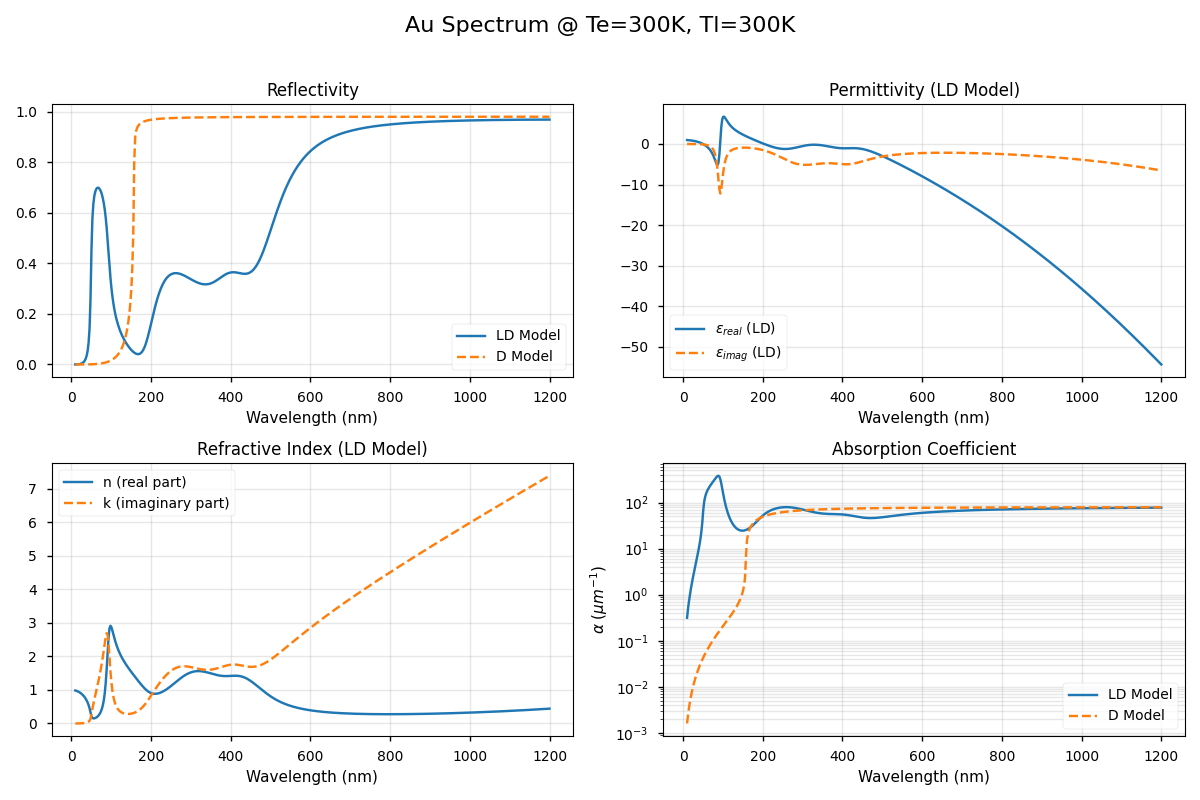
\includegraphics[width=\linewidth,height=3.70cm,keepaspectratio]{../thesis/figures/ch3/spectrum_comparison_10_1200_RT.png}
    \end{minipage}\hspace{0.035\textwidth}
    \begin{minipage}[t]{0.45\textwidth}
      \centering
      {\scriptsize\color{GVSlate}Near-IR operating window}\par
      \vspace{0.04cm}
      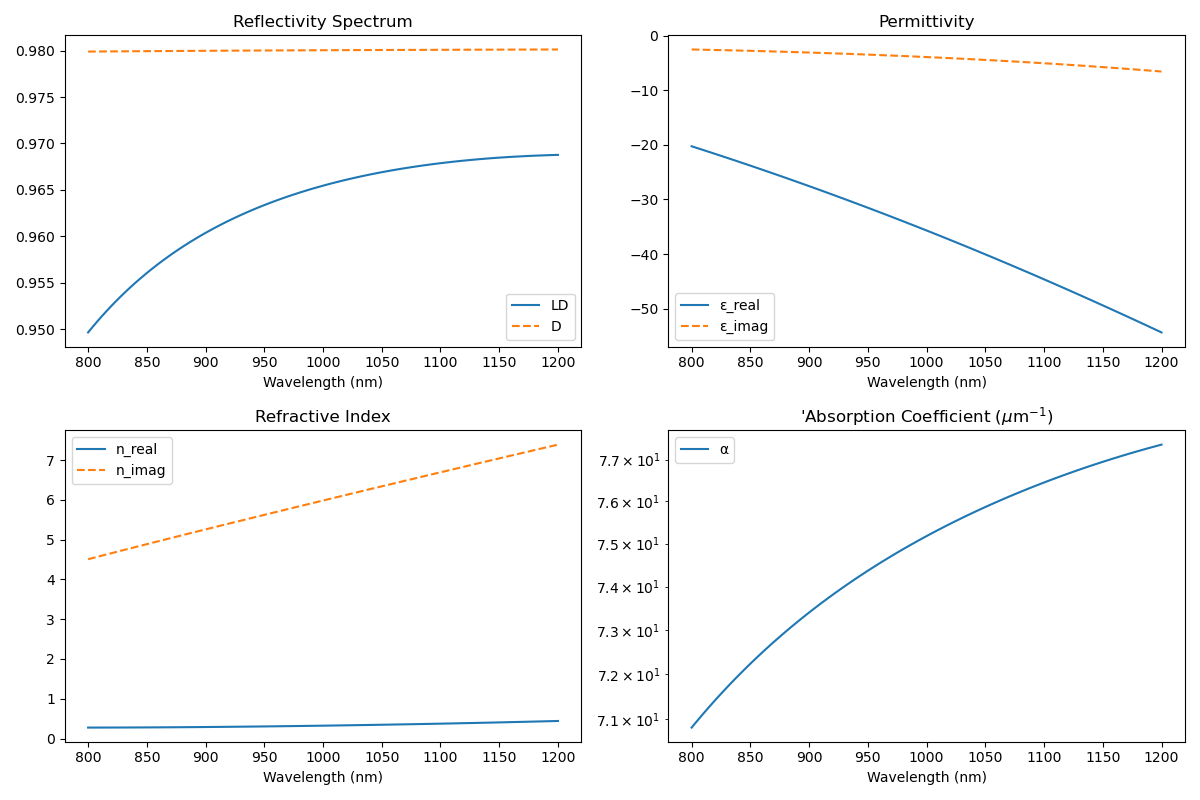
\includegraphics[width=\linewidth,height=3.70cm,keepaspectratio]{../thesis/figures/ch3/spectrum_comparison_RT.png}
    \end{minipage}
  \end{center}
\end{frame}

\GVSetMainSlide{6}
\GVSetSource{Source: thesis Chs. 1 and 3; Fang\_2012.}
\begin{frame}[t]{Thermophysical closures: \(C_e(T_e)\) and \(G(T_e)\)}
  \vspace{-0.18cm}
  \scriptsize
  \[
    \begin{aligned}
    C_e(T_e)&=
    \begin{cases}
      p_{\mathrm{low}}(T_e), & T_e\le T_{\mathrm{th}},\\
      p_{\mathrm{high}}(T_e), & T_e>T_{\mathrm{th}},
    \end{cases}
    \qquad
    G(T_e)=
    \begin{cases}
      q_{\mathrm{low}}(T_e), & T_e\le T_{\mathrm{th}},\\
      q_{\mathrm{high}}(T_e), & T_e>T_{\mathrm{th}}.
    \end{cases}
    \end{aligned}
  \]
  \vspace{-0.24cm}
  \begin{center}
    \textcolor{GVCapacityPurple}{\(C_e\)}: electronic energy storage
    \quad\textbar\quad
    \textcolor{GVCouplingOrange}{\(G\)}: electron--lattice transfer rate
  \end{center}
  \vspace{-0.10cm}
  \begin{columns}[T,totalwidth=0.96\textwidth]
    \begin{column}{0.66\textwidth}
      \centering
      {\scriptsize\color{GVSlate}Focused Au fit over the simulation-relevant threshold window.}\par
      \vspace{0.02cm}
      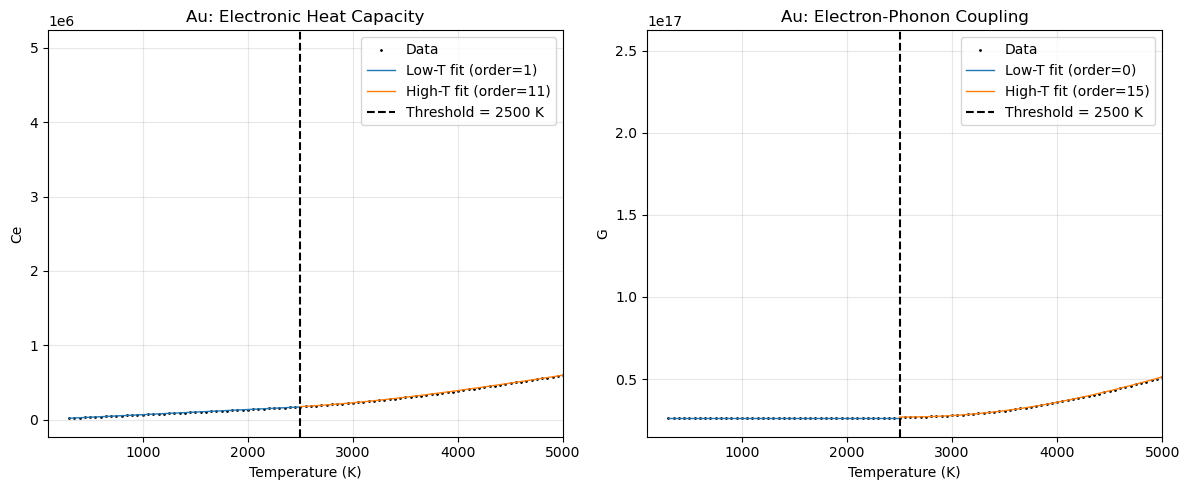
\includegraphics[width=\linewidth]{../thesis/figures/ch3/Au_Ce_G_curves_focused.png}
    \end{column}
    \begin{column}{0.28\textwidth}
      \begin{beamercolorbox}[wd=\linewidth,sep=0.35em]{normal text}
        \centering\tiny
        \textbf{\color{GVTeal}Table 3.3: fit partitions}\\[-0.10em]
        \renewcommand{\arraystretch}{1.10}
        \begin{tabular}{@{}c c c c@{}}
          \hline
          Mat. & \(T_{\mathrm{th}}\) & \(C_e\) & \(G\) \\
          & (K) & deg. & deg. \\ \hline
          Au & 2500 & (1,11) & (0,15) \\
          Ag & 4250 & (1,11) & (0,15) \\
          Cu & 2250 & (1,11) & (0,15) \\
          Fe & 750  & (1,12) & (0,15) \\
          Ni & 500  & (1,12) & (2,15) \\
          Ti & 1000 & (1,11) & (2,15) \\ \hline
        \end{tabular}
      \end{beamercolorbox}
    \end{column}
  \end{columns}
  \vspace{-0.08cm}
  \begin{center}
    \scriptsize
    \(C_e\approx\gamma T_e\) at low \(T_e\). \(C_l\) is fixed under the Dulong--Petit approximation for Au phonons near and above room temperature; \(k_l=0.01\,k_{e0}\) represents electron-dominated conduction.
  \end{center}
\end{frame}

\GVSetMainSlide{7}
\GVSetSource{Public-source policy; see \texttt{docs/ASSET\_PROVENANCE.md}.}
\begin{frame}[t]{Depth--time variation of \(k_e(T_e,T_l)\)}
  \vspace{-0.20cm}
  \begin{center}
    \scriptsize
    \[
      C_e(T_e)\partial_t T_e
      =
      \GVFocusTerm{GVDiffusionGreen}{\nabla\!\cdot\!\left(k_e(T_e,T_l)\nabla T_e\right)}
      +\cdots,
      \qquad
      k_e(T_e,T_l)
      =
      k_{e0}
      \frac{B_L T_e}{A_eT_e^2+B_LT_l}
    \]
  \end{center}
  \vspace{-0.14cm}
  \begin{center}
    \GVOmissionNotice{Project-generated conductivity output omitted from public source pending complete DeeplIPSS provenance.}
  \end{center}
  \vspace{-0.18cm}
  \begin{center}
    \scriptsize\color{GVCharcoal}
    \(k_e\) varies in depth and time during near-threshold heating.
  \end{center}
\end{frame}

\GVSetMainSlide{8}
\GVSetSource{Source: thesis Ch. 2, Eqs. (2.1)--(2.6).}
\begin{frame}[t]{Dimensionless pTTM IBVP formulation}
  \vspace{-0.16cm}
  \begin{center}
    \scriptsize
    \[
      u=\frac{T_e}{T_{\mathrm{ref}}},\quad
      v=\frac{T_l}{T_{\mathrm{ref}}},\quad
      t^*=\frac{t}{t_{\mathrm{ref}}},\quad
      x^*=\frac{x}{L_{\mathrm{ref}}},\quad
      z^*=\frac{z}{L_{\mathrm{ref}}},
      \qquad L_{\mathrm{ref}}=L_x=L_z.
    \]
  \end{center}
  \vspace{-0.18cm}
  \begin{center}
    \small
    \[
      \begin{aligned}
        \partial_t u
        &=
        D_1(u)\,\nabla\!\cdot\!\left(\textcolor{GVDiffusionGreen}{K(u,v)}\nabla u\right)
        -\textcolor{GVCouplingOrange}{c_1(u)(u-v)}
        +\textcolor{GVSourceBlue}{s(t,\mathbf{x};u,v)},\\[0.55em]
        \partial_t v
        &=
        D_2\nabla^2v
        +\textcolor{GVCouplingOrange}{c_2(u)(u-v)}.
      \end{aligned}
    \]
  \end{center}
  \vspace{-0.08cm}
  \begin{columns}[T,totalwidth=0.94\textwidth]
    \begin{column}{0.48\textwidth}
      \begin{beamercolorbox}[wd=\linewidth,sep=0.56em]{normal text}
        \scriptsize
        \textbf{\color{GVTeal}Spatio-temporal cylinder}\\
          \(Q_{\tau_f}:=\Omega\times(0,\tau_f]\),\quad
        \(\Omega=(0,1)^d\), \(d\in\{1,2\}\).\\[-0.08em]
        The discrete grid includes \(\overline{\Omega}=[0,1]^d\).
      \end{beamercolorbox}
    \end{column}
    \begin{column}{0.42\textwidth}
      \begin{beamercolorbox}[wd=\linewidth,sep=0.56em]{normal text}
        \scriptsize
        \textbf{\color{GVSlate}Cauchy and boundary data}\\
        \(u(\mathbf{x},0)=v(\mathbf{x},0)=u_{\mathrm{RT}}\),\quad \(\mathbf{x}\in\Omega\).\\[-0.08em]
        \(u=v=u_{\mathrm{RT}}\) on \(\partial\Omega\times(0,\tau_f]\).
      \end{beamercolorbox}
    \end{column}
  \end{columns}
  \vspace{0.12cm}
  \begin{center}
    \scriptsize\color{GVSlate}
    Dimensionless coefficient and source definitions inherit the physical closures introduced on Slides 4--7.
  \end{center}
\end{frame}

\GVSetMainSlide{9}
\GVSetSource{Source: thesis Ch. 2, Eqs. (2.22)--(2.23), \S2.5.4; Kadioglu\_2008.}
\begin{frame}[t]{2D finite-difference discretisation of electron heat diffusion}
  \vspace{-0.18cm}
  \begin{columns}[T,totalwidth=0.99\textwidth]
    \begin{column}{0.54\textwidth}
      \centering
      \begin{tikzpicture}[>=stealth,x=1.17cm,y=1.035cm]
        \fill[GVTealTint] (1.5,1.5) rectangle (2.5,2.5);
        \foreach \x in {0,1,2,3,4} {
          \draw[color=GVSlate!55,line width=0.42pt] (\x,0) -- (\x,4);
        }
        \foreach \y in {0,1,2,3,4} {
          \draw[color=GVSlate!55,line width=0.42pt] (0,\y) -- (4,\y);
        }
        \draw[GVDiffusionGreen!70,densely dotted,line width=0.45pt]
          (1.5,0.25) -- (1.5,3.75) (2.5,0.25) -- (2.5,3.75)
          (0.25,1.5) -- (3.75,1.5) (0.25,2.5) -- (3.75,2.5);
        \draw[GVTitleRed,densely dashed,line width=0.65pt] (1.5,1.5) rectangle (2.5,2.5);
        \foreach \x in {0,1,2,3,4} {
          \foreach \y in {0,1,2,3,4} {
            \fill[GVCharcoal] (\x,\y) circle (1.15pt);
          }
        }
        \fill[GVSourceBlue] (2,2) circle (1.90pt);
        \foreach \x/\y in {1.5/2,2.5/2,2/1.5,2/2.5} {
          \draw[GVDiffusionGreen,fill=GVCanvas,line width=0.65pt] (\x,\y) circle (2.15pt);
        }
        \draw[GVDiffusionGreen,line width=0.8pt] (2.08,2) -- (2.44,2);
        \draw[GVDiffusionGreen,line width=0.8pt] (1.92,2) -- (1.56,2);
        \draw[GVDiffusionGreen,line width=0.8pt] (2,2.08) -- (2,2.44);
        \draw[GVDiffusionGreen,line width=0.8pt] (2,1.92) -- (2,1.56);
        \node[font=\scriptsize,anchor=north west] at (2.08,1.86) {\(u_{i,j}\)};
        \node[font=\scriptsize,anchor=east] at (0.90,1.74) {\(u_{i-1,j}\)};
        \node[font=\scriptsize,anchor=west] at (3.10,1.74) {\(u_{i+1,j}\)};
        \node[font=\scriptsize,anchor=north] at (2,0.84) {\(u_{i,j-1}\)};
        \node[font=\scriptsize,anchor=south] at (2,3.18) {\(u_{i,j+1}\)};
        \draw[GVDiffusionGreen!72,line width=0.35pt] (1.5,2) -- (0.86,2.58);
        \node[font=\scriptsize,text=GVDiffusionGreen,anchor=east] at (0.84,2.60) {\(q^x_e\)};
        \draw[GVDiffusionGreen!72,line width=0.35pt] (2.5,2) -- (3.16,2.58);
        \node[font=\scriptsize,text=GVDiffusionGreen,anchor=west] at (3.18,2.60) {\(q^x_e\)};
        \draw[GVDiffusionGreen!72,line width=0.35pt] (2,2.5) -- (1.22,3.02);
        \node[font=\scriptsize,text=GVDiffusionGreen,anchor=east] at (1.20,3.04) {\(q^z_e\)};
        \draw[GVDiffusionGreen!72,line width=0.35pt] (2,1.5) -- (3.06,1.02);
        \node[font=\scriptsize,text=GVDiffusionGreen,anchor=west] at (3.08,1.00) {\(q^z_e\)};
        \draw[->,GVTitleRed,line width=0.55pt] (3.58,3.52) -- (2.52,2.52)
          node[pos=0.08,right,font=\scriptsize,text=GVTitleRed] {control volume};
        \draw[<->,GVSlate,line width=0.45pt] (1.5,-0.26) -- (2.5,-0.26)
          node[midway,below,font=\scriptsize] {\(\Delta_x\)};
        \draw[<->,GVSlate,line width=0.45pt] (4.18,1.5) -- (4.18,2.5)
          node[midway,right,font=\scriptsize] {\(\Delta_z\)};
      \end{tikzpicture}
      \vspace{-0.12cm}
      \begin{center}
        \scriptsize\color{GVSlate}
        Cell-centred temperatures; face-centred electron heat fluxes.
      \end{center}
    \end{column}
    \begin{column}{0.42\textwidth}
      \scriptsize
      \setlength{\abovedisplayskip}{0.18em}
      \setlength{\belowdisplayskip}{0.18em}
      \setlength{\abovedisplayshortskip}{0.16em}
      \setlength{\belowdisplayshortskip}{0.16em}
      \setlength{\arraycolsep}{1.9pt}
      \begingroup
      \setlength{\fboxsep}{0.35em}
      \noindent\colorbox{GVTealTint}{%
        \begin{minipage}{\dimexpr\linewidth-2\fboxsep\relax}
          \scriptsize\textbf{\color{GVTeal}Nonlinear operator action}
          \[
            D_1(u)\nabla\!\cdot(K\nabla u)
            \;\longrightarrow\;
            D_1(u)\mathcal{K}(K)[u].
          \]
        \end{minipage}}
      \endgroup

      \vspace{0.28cm}
      \begingroup
      \setlength{\fboxsep}{0.35em}
      \noindent\colorbox{GVTealTint}{%
        \begin{minipage}{\dimexpr\linewidth-2\fboxsep\relax}
          \scriptsize\textbf{\color{GVTeal}Evaluation order}
          \[
            \begin{aligned}
              \text{1.}\quad
              \textcolor{GVDiffusionGreen}{K_{i+\frac12,j}}
              &=
              \frac{\textcolor{GVDiffusionGreen}{K_{i,j}}+\textcolor{GVDiffusionGreen}{K_{i+1,j}}}{2},\\[-0.03em]
              \text{2.}\quad q^x_{e,i+\frac12,j}
              &=
              -\textcolor{GVDiffusionGreen}{K_{i+\frac12,j}}
              \frac{u_{i+1,j}-u_{i,j}}{\Delta_x},\\[-0.03em]
              \text{3.}\quad \mathcal{K}(K)[u]_{i,j}
              &:=
              -(\nabla_h\!\cdot\mathbf q_{e,h})_{i,j}.
            \end{aligned}
          \]
          {\scriptsize\color{GVSlate}\(q^z_e\) is defined analogously.}
        \end{minipage}}
      \endgroup

      \vspace{0.28cm}
      \begingroup
      \setlength{\fboxsep}{0.35em}
      \noindent\colorbox{GVTealTint}{%
        \begin{minipage}{\dimexpr\linewidth-2\fboxsep\relax}
          \scriptsize\textbf{\color{GVTeal}Central 2D Laplacian}
          {\scriptsize\color{GVSlate}\par Constant \(K\): \(\mathcal{K}(K)[u]=K\mathcal{L}[u]\).}
          \[
            \begin{aligned}
              \mathcal{L}[u]_{i,j}
              &=
              \frac{u_{i+1,j}-2u_{i,j}+u_{i-1,j}}{\Delta_x^2}\\[-0.06em]
              &\quad+
              \frac{u_{i,j+1}-2u_{i,j}+u_{i,j-1}}{\Delta_z^2}.
            \end{aligned}
          \]
        \end{minipage}}
      \endgroup
    \end{column}
  \end{columns}
\end{frame}

\GVSetMainSlide{10}
\GVSetSource{Source: thesis Ch. 2, \S2.4.2, Eqs. (2.26)--(2.31).}
\begin{frame}[t]{Linear pTTM: monolithic Crank--Nicolson system}
  \vspace{-0.16cm}
  \begin{center}
    \scriptsize
    \[
      \dot{\boldsymbol{\theta}}=\mathbf{R}(\boldsymbol{\theta},t),
      \qquad
      \boldsymbol{\theta}=
      \begin{bmatrix}\mathbf u\\\mathbf v\end{bmatrix}
      \quad
      \xrightarrow{\ \mathrm{Crank\!-\!Nicolson}\ }\quad
      \boldsymbol{\theta}^{n+1}
      =
      \boldsymbol{\theta}^{n}
      +
      \frac{\Delta_t}{2}
      \left[
        \mathbf{R}(\boldsymbol{\theta}^{n},t^n)
        +
        \mathbf{R}(\boldsymbol{\theta}^{n+1},t^{n+1})
      \right].
    \]
  \end{center}
  \vspace{-0.20cm}
  \begin{columns}[T,totalwidth=0.96\textwidth]
    \begin{column}{0.63\textwidth}
      \centering
      \normalsize
      \[
        \begin{bmatrix}
          \mathbf A_e^{(2D)}+c_e\mathbf I & -c_e\mathbf I\\[0.15em]
          -c_l\mathbf I & \mathbf A_l^{(2D)}+c_l\mathbf I
        \end{bmatrix}
        \begin{bmatrix}
          \mathbf u^{n+1}\\[0.15em]
          \mathbf v^{n+1}
        \end{bmatrix}
        =
        \begin{bmatrix}
          \mathbf b_e\\[0.15em]
          \mathbf b_l
        \end{bmatrix}.
      \]
      \vspace{-0.12cm}
      \scriptsize
      \[
        \mathbf A_e^{(2D)}=\mathbf I-\frac12D_1\Delta_t\mathbf L_{2D},
        \qquad
        \mathbf A_l^{(2D)}=\mathbf I-\frac12D_2\Delta_t\mathbf L_{2D}.
      \]
      \vspace{-0.22cm}
      \[
        \mathbf L_{2D}=\mathbf I_{N_z}\otimes\mathbf L_x+\mathbf L_z\otimes\mathbf I_{N_x}.
      \]
    \end{column}
    \begin{column}{0.29\textwidth}
      \begin{beamercolorbox}[wd=\linewidth,sep=0.46em]{normal text}
        \scriptsize
        \textbf{\color{GVTeal}Vectorised fields}\\
        \(M=N_xN_z\) unknowns per thermal field.
      \end{beamercolorbox}
      \vspace{0.10cm}
      \begin{beamercolorbox}[wd=\linewidth,sep=0.46em]{normal text}
        \scriptsize
        \textbf{\color{GVCouplingOrange}Off-diagonal blocks}\\
        Electron--lattice coupling remains monolithic.
      \end{beamercolorbox}
      \vspace{0.10cm}
      \begin{beamercolorbox}[wd=\linewidth,sep=0.46em]{normal text}
        \scriptsize
        \textbf{\color{GVDiffusionGreen}Sparse solve}\\
        The Kronecker Laplacian supplies the 2D transport operator.
      \end{beamercolorbox}
    \end{column}
  \end{columns}
  \vspace{0.12cm}
  \begin{center}
    \scriptsize\color{GVSlate}
    Frozen transport and coupling coefficients define the linear reference; source dependence can still require Picard iteration.
  \end{center}
\end{frame}

\GVSetMainSlide{11}
\GVSetSource{Source: thesis Ch. 2, \S2.5; Ascher\_1997; Huang\_2019.}
\begin{frame}[t]{Nonlinear pTTM: IMEX Heun/Crank--Nicolson split}
  \vspace{-0.16cm}
  \begin{center}
    \small
    \[
      \mathbf F(\boldsymbol\theta,t)
      =
      \underbrace{\textcolor{GVDiffusionGreen}{\mathbf D(\boldsymbol\theta)}}_{\text{implicit diffusion}}
      +
      \underbrace{\textcolor{GVCouplingOrange}{\mathbf C(\boldsymbol\theta)}}_{\text{implicit coupling}}
      +
      \underbrace{\textcolor{GVSourceBlue}{\mathbf S(t,\boldsymbol\theta)}}_{\text{explicit source}}.
    \]
  \end{center}
  \vspace{-0.05cm}
  \begin{center}
    \begin{tikzpicture}[
      >=stealth,
      stage/.style={
        draw=GVTeal,
        fill=GVTealTint,
        rounded corners=2pt,
        align=center,
        text width=2.35cm,
        minimum height=1.05cm,
        font=\scriptsize
      },
      arrow/.style={->,color=GVSlate,line width=0.55pt}
    ]
      \node[stage] (old) {old state\\[-0.10em]\((\mathbf u^n,\mathbf v^n)\)};
      \node[stage,right=0.42cm of old] (electron) {electron stage\\[-0.10em]lagged \(\mathbf v^n\)};
      \node[stage,right=0.42cm of electron] (lattice) {lattice stage\\[-0.10em]updated electron field};
      \node[stage,right=0.42cm of lattice] (new) {new state\\[-0.10em]\((\mathbf u^{n+1},\mathbf v^{n+1})\)};
      \draw[arrow] (old) -- (electron);
      \draw[arrow] (electron) -- (lattice);
      \draw[arrow] (lattice) -- (new);
    \end{tikzpicture}
  \end{center}
  \vspace{0.10cm}
  \begin{columns}[T,totalwidth=0.93\textwidth]
    \begin{column}{0.29\textwidth}
      \begin{beamercolorbox}[wd=\linewidth,sep=0.48em]{normal text}
        \scriptsize
        \textbf{\color{GVDiffusionGreen}Implicit}\\
        Nonlinear diffusion controls the restrictive stiffness scale.
      \end{beamercolorbox}
    \end{column}
    \begin{column}{0.29\textwidth}
      \begin{beamercolorbox}[wd=\linewidth,sep=0.48em]{normal text}
        \scriptsize
        \textbf{\color{GVCouplingOrange}Implicit}\\
        Electron--lattice coupling stays within the sequential stiff solve.
      \end{beamercolorbox}
    \end{column}
    \begin{column}{0.29\textwidth}
      \begin{beamercolorbox}[wd=\linewidth,sep=0.48em]{normal text}
        \scriptsize
        \textbf{\color{GVSourceBlue}Explicit}\\
        The laser source is advanced by the Heun part.
      \end{beamercolorbox}
    \end{column}
  \end{columns}
  \vspace{0.10cm}
  \begin{center}
    \scriptsize\color{GVSlate}
    The strong Gauss--Seidel predictor creates the electron-first, lattice-second dependency.
  \end{center}
\end{frame}

\GVSetMainSlide{12}
\GVSetSource{Source: thesis Ch. 2, \S2.4.3; Pollock\_2018.}
\begin{frame}[t]{Picard fixed-point solves accelerated by Anderson mixing}
  \vspace{-0.18cm}
  \begin{center}
    \begin{tikzpicture}[
      >=stealth,
      node/.style={
        draw=GVTeal,
        fill=GVTealTint,
        rounded corners=2pt,
        align=center,
        text width=2.42cm,
        minimum height=0.82cm,
        font=\small
      },
      arrow/.style={->,color=GVSlate,line width=0.55pt}
    ]
      \node[node] (iterate) {current iterate\\[-0.12em]\(\boldsymbol{\theta}^{(k)}\)};
      \node[node,right=0.36cm of iterate] (assemble) {assemble coefficients\\and source};
      \node[node,right=0.36cm of assemble] (solve) {sparse solve and\\raw residual};
      \node[node,right=0.36cm of solve] (anderson) {Anderson mixing\\convergence test};
      \draw[arrow] (iterate) -- (assemble);
      \draw[arrow] (assemble) -- (solve);
      \draw[arrow] (solve) -- (anderson);
      \draw[arrow] (anderson.north west) -- ++(0,0.26)
        -| node[pos=0.26,above,font=\scriptsize,color=GVSlate] {next iterate} (iterate.north);
    \end{tikzpicture}
  \end{center}
  \vspace{-0.10cm}
  \begin{columns}[T,totalwidth=0.94\textwidth]
    \begin{column}{0.39\textwidth}
      \begin{beamercolorbox}[wd=\linewidth,sep=0.44em]{normal text}
        \small
        \textbf{\color{GVTeal}Residual and history}\\[0.10em]
        \(\boldsymbol{\theta}_{\mathrm{raw}}^{(k+1)}=\mathcal F(\boldsymbol{\theta}^{(k)})\).\\[-0.08em]
        \(\mathbf f^{(k)}=\boldsymbol{\theta}_{\mathrm{raw}}^{(k+1)}-\boldsymbol{\theta}^{(k)}\).\\[-0.10em]
        \(\Delta\mathbf F\): residual differences.\\[-0.10em]
        \(\Delta\boldsymbol{\Theta}\): iterate differences.
      \end{beamercolorbox}
    \end{column}
    \begin{column}{0.51\textwidth}
      \scriptsize
      \[
        \boldsymbol\gamma
        =
        \arg\min_{\boldsymbol\alpha}
        \left\{
          \|\Delta\mathbf F\boldsymbol\alpha-\mathbf f^{(k)}\|_2^2
          +\epsilon\|\boldsymbol\alpha\|_2^2
        \right\},
      \]
      \vspace{-0.24cm}
      \[
        \boldsymbol{\theta}^{(k+1)}
        =
        \boldsymbol{\theta}_{\mathrm{raw}}^{(k+1)}
        -\Delta\boldsymbol{\Theta}\boldsymbol\gamma.
      \]
      \vspace{-0.10cm}
      \scriptsize\color{GVSlate}
      Anderson mixing accelerates the Picard map without changing the converged discrete problem.
    \end{column}
  \end{columns}
  \begin{tikzpicture}[remember picture,overlay]
    \node[anchor=south] at ([yshift=0.47cm]current page.south) {%
      \begin{minipage}{0.48\textwidth}
        \begin{beamercolorbox}[wd=\linewidth,sep=0.46em,center]{normal text}
          \small
          \textbf{\color{GVSlate}Retained controls}\\[0.10em]
          {\scriptsize
          \renewcommand{\arraystretch}{1.12}%
          \begin{tabular}{@{}r@{\;\(\mapsto\)\;}l@{}}
            \textcolor{GVTitleRed}{\(m=5\)} & history depth \\
            \textcolor{GVTitleRed}{\(\tau_{\mathrm P}=10^{-6}\)} & Picard tolerance \\
            \textcolor{GVTitleRed}{\(\epsilon=10^{-8}\)} & regularisation \\
            \textcolor{GVTitleRed}{\(\beta=1\)} & full relaxation
          \end{tabular}}
        \end{beamercolorbox}
      \end{minipage}%
    };
  \end{tikzpicture}
\end{frame}

\GVSetMainSlide{13}
\GVSetSource{Source: thesis Ch. 2, Eqs. (2.42)--(2.45).}
\begin{frame}[t]{Stiffness scales motivate the IMEX partition}
  \vspace{-0.10cm}
  \begin{center}
    \begin{beamercolorbox}[wd=0.90\textwidth,sep=0.42em,center]{normal text}
      \resizebox{0.96\linewidth}{!}{%
      \(\displaystyle
        \dot{u}
        \approx
        D_1(u)\frac{K(u,v)}{\Delta_x^2}\mathcal{L}[u]
        -c_1(u)(u-v)
        +
        \alpha'(u,v)\bigl(1-R(u,v)\bigr)\frac{F^*}{t_p}g(\mathbf{x},t;u,v).
      \)}
    \end{beamercolorbox}

    \vspace{0.22cm}

    \begin{beamercolorbox}[wd=0.84\textwidth,sep=0.58em,center]{normal text}
      {\large\textbf{\color{GVTeal}Leading coefficient scales}}\par
      \vspace{0.12cm}
      \resizebox{0.96\linewidth}{!}{%
      \(\displaystyle
        \begin{aligned}
          q_1(t,\mathbf{x})
          &=
          D_1(u)\frac{K(u,v)}{\Delta_x^2},
          &
          q_2(t,\mathbf{x};F^*)
          &=
          -c_1(u)+
          \alpha'(u,v)(1-R(u,v))\frac{F^*}{t_p},\\[0.58em]
          \lambda(t;F^*)
          &=
          \max_{\mathbf{x}\in\Omega}
          \frac{q_1(t,\mathbf{x})}{q_2(t,\mathbf{x};F^*)},
          &
          \lambda_{\min/\max}(F^*)
          &=
          \min/\max_{t\in[0,\tau_f]}\lambda(t;F^*).
        \end{aligned}
      \)}
    \end{beamercolorbox}

    \vspace{0.18cm}

    \begin{beamercolorbox}[wd=0.92\textwidth,sep=0.55em,center]{normal text}
      \small
      \(\lambda\gg1\): diffusion-dominated stiffness
      \quad\textbar\quad
      \(\lambda\ll1\): reaction/source scale dominates.
    \end{beamercolorbox}
  \end{center}
\end{frame}

\GVSetMainSlide{14}
\GVSetSource{Source: thesis Ch. 2, Fig. 2.1, Eqs. (2.42)--(2.45), Table 2.7.}
\begin{frame}[t]{Stiffness scales motivate the IMEX partition}
  \vspace{-0.18cm}
  \begin{columns}[T,totalwidth=1.00\textwidth]
    \begin{column}{0.75\textwidth}
      \centering
      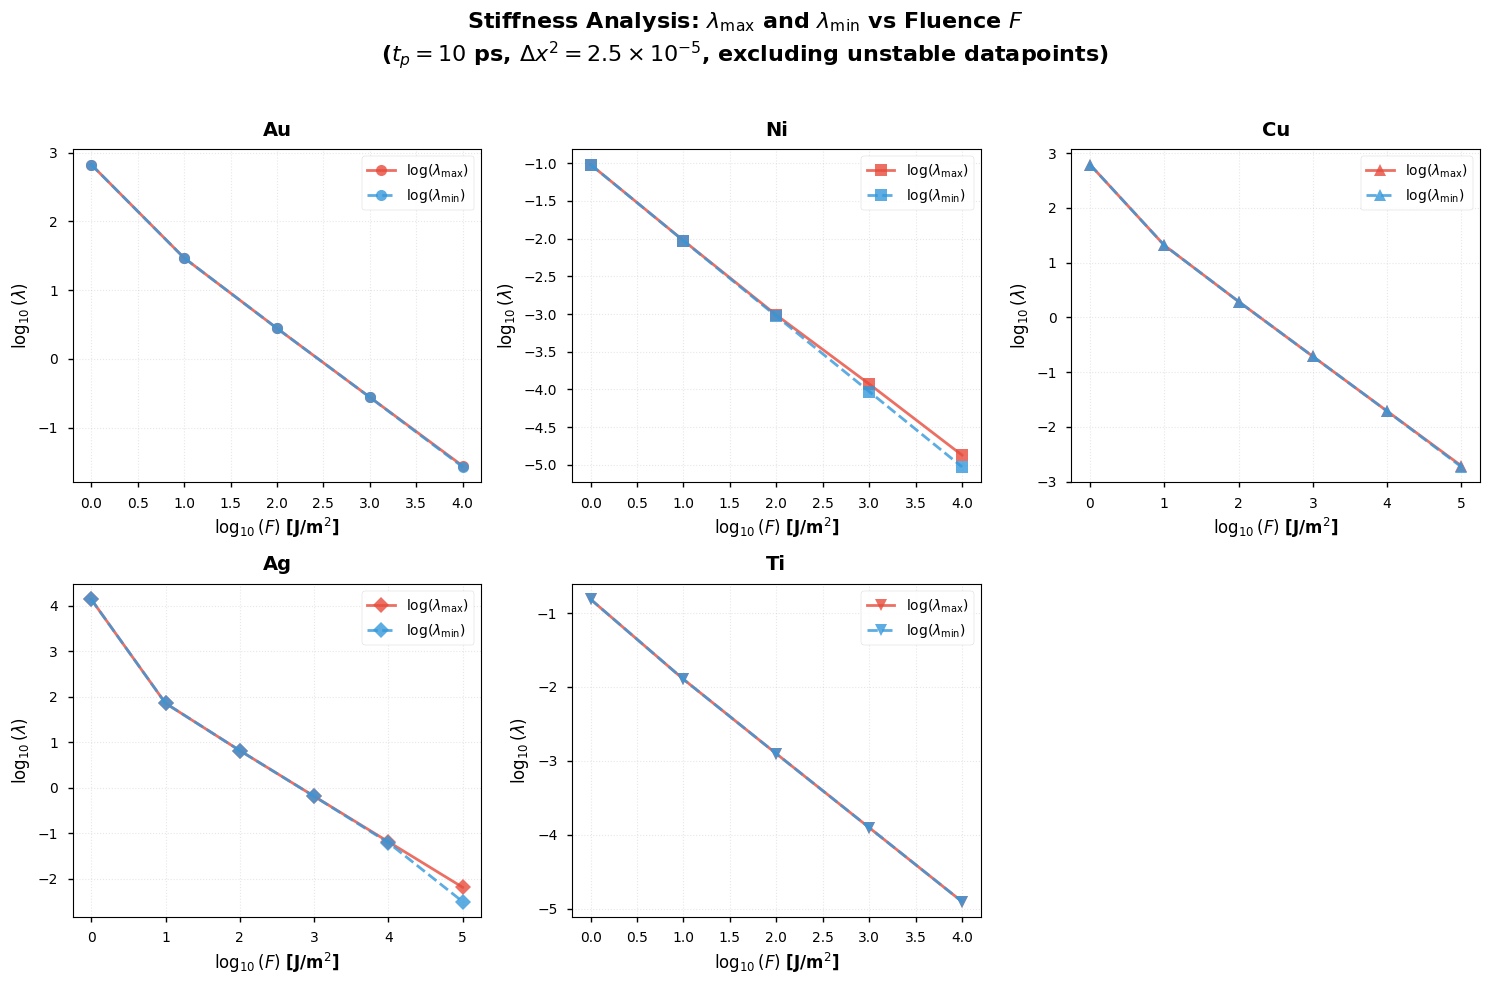
\includegraphics[
        width=\linewidth,
        height=5.78cm,
        keepaspectratio
      ]{../thesis/figures/ch2/stiffness_plots.png}
      \vspace{-0.10cm}
      {\scriptsize\color{GVSlate}
        \parbox{0.96\linewidth}{\centering
          Stiffness quotient over fluence and pulse duration.\\[-0.04em]
          \(\lambda_{\min}\) and \(\lambda_{\max}\) bracket the transient regime.}}
    \end{column}
    \begin{column}{0.25\textwidth}
      {\scriptsize\textbf{\color{GVTeal}Leading coefficient scales}\par}
      \vspace{0.04cm}
      {\tiny
        \(\displaystyle q_1(t,\mathbf{x})=
        D_1(u)\frac{K(u,v)}{\Delta_x^2}\).\\[0.24em]
        \(\displaystyle q_2(t,\mathbf{x};F^*)=
        -c_1(u)+
        \alpha'(u,v)(1-R(u,v))\frac{F^*}{t_p}\).\\[0.28em]
        \(\displaystyle \lambda(t;F^*)=
        \max_{\mathbf{x}\in\Omega}
        \frac{q_1(t,\mathbf{x})}{q_2(t,\mathbf{x};F^*)}\).\\[0.56em]
        \resizebox{\linewidth}{!}{%
          \(\lambda_{\min/\max}=
          \min/\max_{t\in[0,\tau_f]}\lambda(t;F^*)\).%
        }\\[0.34em]
        \(\lambda\gg1\): diffusion; \(\lambda\ll1\): reaction/source.\par
      }
      \vspace{0.16cm}
      \begin{beamercolorbox}[wd=\linewidth,sep=0.26em]{normal text}
        \centering\tiny
        {\scriptsize\textbf{\color{GVTitleRed}Au solver cost}}\\[0.10em]
        \renewcommand{\arraystretch}{1.04}
        \begin{tabular}{@{}l r r@{}}
          \hline
          \rowcolor{black!12}
          Case & steps & total (s) \\ \hline
          1D linear & 1000 & 2.92 \\
          2D linear & 200 & 5.60 \\
          1D nonlinear & 1000 & 26.39 \\
          2D nonlinear & 200 & 54.65 \\ \hline
        \end{tabular}\\[-0.05em]
        \tiny\color{GVSlate}Au benchmark; stated local CPU.
      \end{beamercolorbox}
    \end{column}
  \end{columns}
\end{frame}

\GVSetMainSlide{15}
\GVSetSource{Source: thesis Ch. 2, Fig. 2.2; Tables 2.9--2.11.}
\begin{frame}[t]{Refinement and runtime validation select the retained split}
  \vspace{-0.16cm}
  \begin{center}
    \begin{tikzpicture}[
      claim/.style={
        draw=GVTeal,
        fill=GVTealTint,
        rounded corners=2pt,
        align=center,
        text width=3.28cm,
        minimum height=0.68cm,
        font=\scriptsize
      }
    ]
      \node[claim] (variant) {{\color{GVCouplingOrange}\textbf{Variant 2}}\\implicit diffusion + coupling;\\explicit source};
      \node[claim,right=0.30cm of variant] (order) {\textbf{Observed second order}\\time \(p\approx2.001\) \quad space \(q\approx2.012\)};
      \node[claim,right=0.30cm of order] (runtime) {\textbf{Runtime evidence}\\\(23.71\) vs \(27.27\,\mathrm{s}\): \underline{\(1.15\times\) faster}};
    \end{tikzpicture}
  \end{center}
  \vspace{-0.08cm}
  \begin{columns}[T,totalwidth=0.96\textwidth]
    \begin{column}{0.47\textwidth}
      \centering
      {\scriptsize\color{GVSlate}Temporal refinement}\par
      \vspace{0.04cm}
      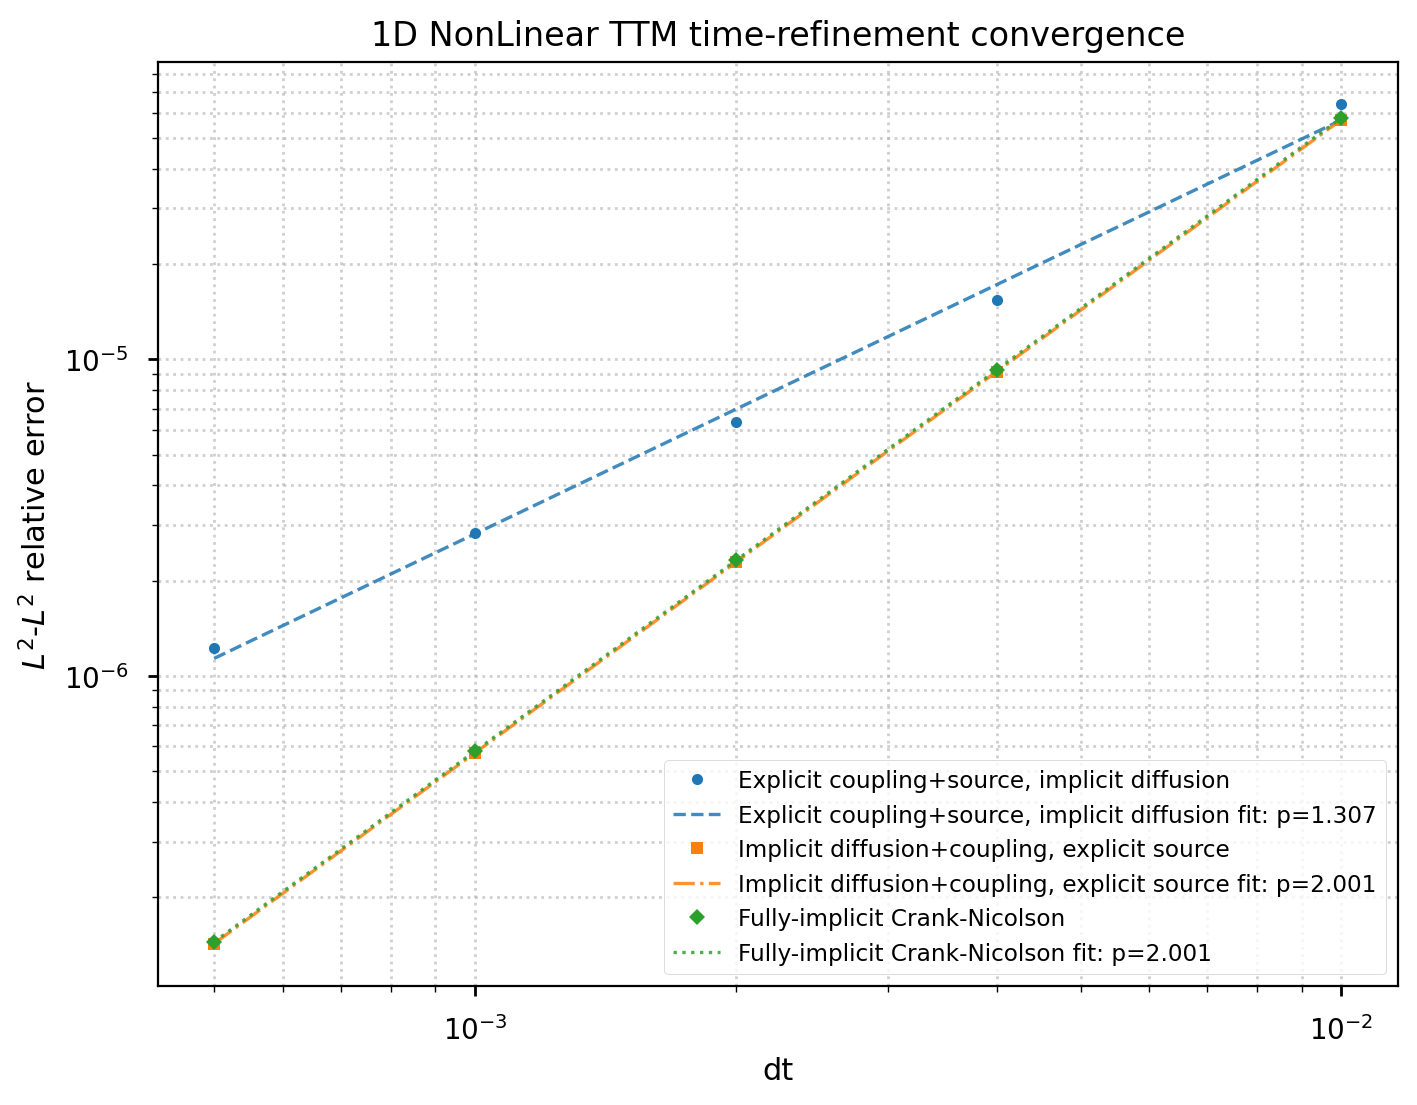
\includegraphics[width=\linewidth,height=4.22cm,keepaspectratio]{../thesis/figures/ch2/time_convergence.png}
    \end{column}
    \begin{column}{0.47\textwidth}
      \centering
      {\scriptsize\color{GVSlate}Spatial refinement}\par
      \vspace{0.04cm}
      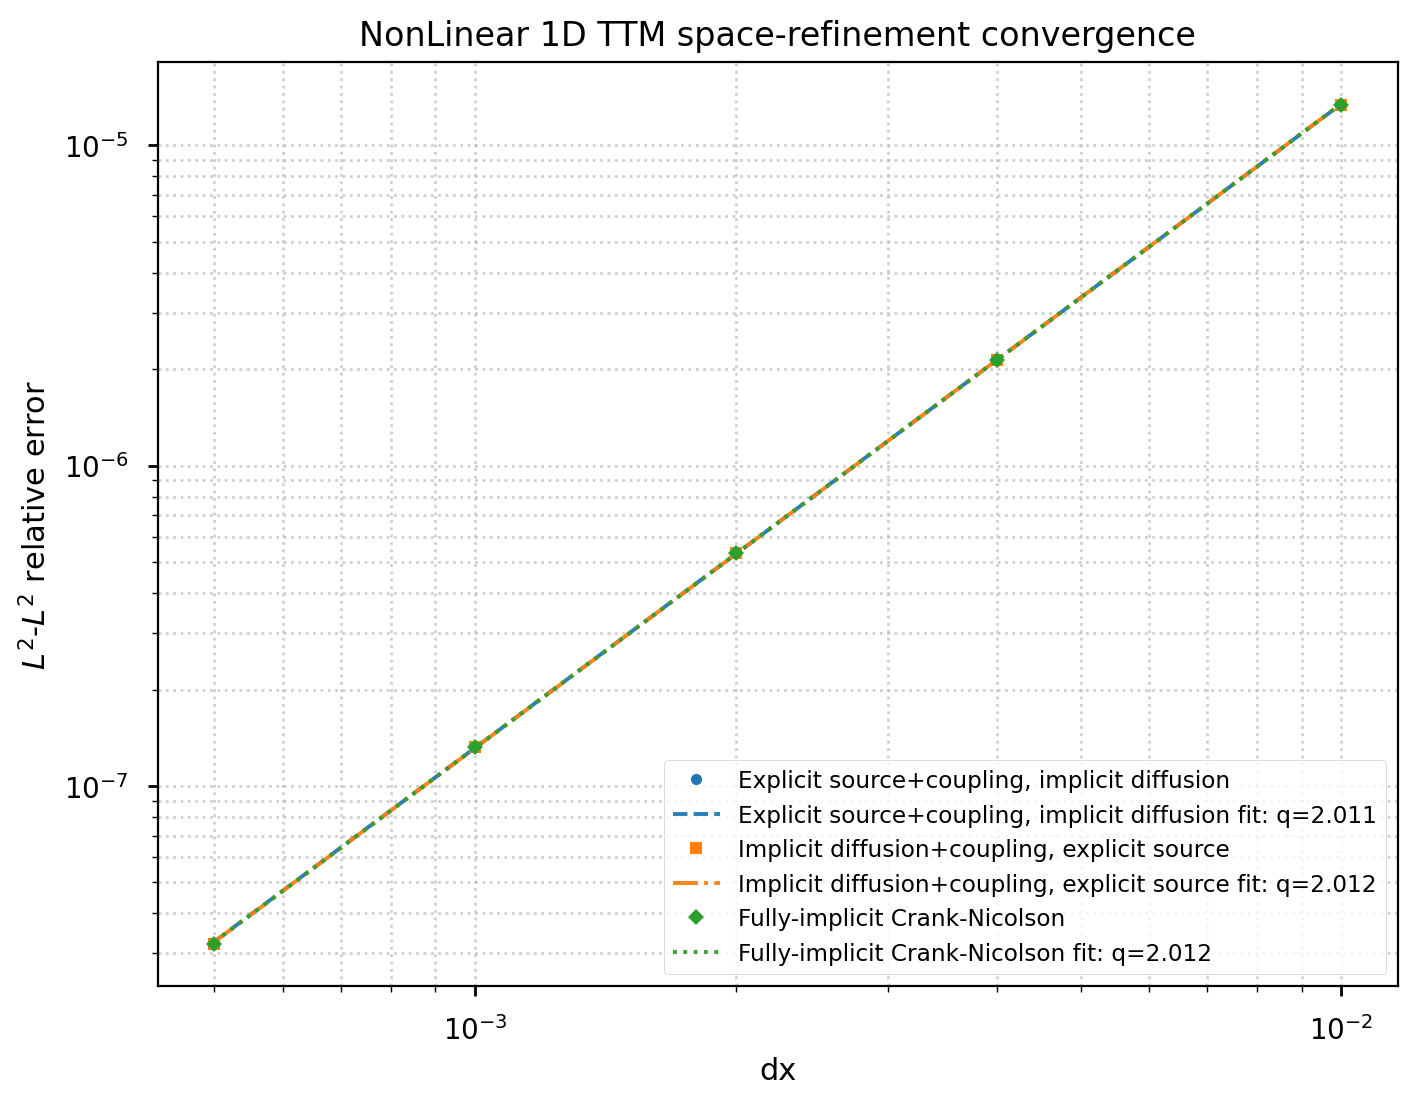
\includegraphics[width=\linewidth,height=4.22cm,keepaspectratio]{../thesis/figures/ch2/space_convergence.png}
    \end{column}
  \end{columns}
  \vspace{-0.10cm}
  \begin{center}
    \scriptsize\color{GVSlate}
    Treating the source explicitly avoids source-Jacobian assembly and an implicit source solve in the tested nonlinear configuration.
  \end{center}
\end{frame}

\GVSetMainSlide{16}
\GVSetSource{Source: thesis Ch. 4, Table 4.1; Appendix C, Table C.1.}
\begin{frame}[t]{Synthetic 2D pTTM datasets: support and acceptance}
  \vspace{-0.14cm}
  \begin{columns}[T,totalwidth=0.96\textwidth]
    \begin{column}{0.47\textwidth}
      \begin{beamercolorbox}[wd=\linewidth,sep=0.48em]{normal text}
        \centering
        \small\textbf{\color{GVTeal}Linear route}\par
        \vspace{0.10cm}
        \begin{tikzpicture}[
          >=stealth,
          count/.style={
            draw=GVTeal,
            fill=GVTealTint,
            rounded corners=2pt,
            align=center,
            minimum width=1.46cm,
            minimum height=0.78cm,
            font=\scriptsize
          },
          arrow/.style={->,color=GVSlate,line width=0.5pt}
        ]
          \node[count] (requested) {300,000\\requested};
          \node[count,right=0.22cm of requested] (finite) {92.6\%\\finite};
          \node[count,right=0.22cm of finite] (retained) {65.0\% of\\requests retained};
          \draw[arrow] (requested) -- (finite);
          \draw[arrow] (finite) -- (retained);
        \end{tikzpicture}
        \vspace{0.08cm}

        {\scriptsize
          \textbf{Split:} 80\% train \(\mid\) 10\% validation \(\mid\) 10\% test.\par
          \vspace{0.08cm}
          \textbf{Generation grid:} \(N_x=N_z=101,\;N_t=501\).\par
          \vspace{0.08cm}
          \colorbox{GVRedTint}{\strut finite response and \(T_{l,\max}\leq10^4\,\mathrm K\)}
        }
      \end{beamercolorbox}
    \end{column}
    \begin{column}{0.47\textwidth}
      \begin{beamercolorbox}[wd=\linewidth,sep=0.48em]{normal text}
        \centering
        \small\textbf{\color{GVDiffusionGreen}Nonlinear route}\par
        \vspace{0.10cm}
        \begin{tikzpicture}[
          >=stealth,
          count/.style={
            draw=GVDiffusionGreen,
            fill=GVTealTint,
            rounded corners=2pt,
            align=center,
            minimum width=2.00cm,
            minimum height=0.78cm,
            font=\scriptsize
          },
          arrow/.style={->,color=GVSlate,line width=0.5pt}
        ]
          \node[count] (accepted) {20,000\\accepted target};
          \node[count,right=0.48cm of accepted] (yield) {90.3\%\\acceptance yield};
          \draw[arrow] (accepted) -- (yield);
        \end{tikzpicture}
        \vspace{0.08cm}

        {\scriptsize
          \textbf{Split:} 80\% train \(\mid\) 20\% test.\par
          \vspace{0.08cm}
          \textbf{Generation grid:} \(N_x=N_z=101,\;N_t=201\).
        }
      \end{beamercolorbox}
    \end{column}
  \end{columns}

  \vspace{0.12cm}
  \begin{columns}[T,totalwidth=0.96\textwidth]
    \begin{column}{0.47\textwidth}
      \begin{beamercolorbox}[wd=\linewidth,sep=0.52em]{normal text}
        \scriptsize
        \textbf{\color{GVTeal}Direct sampled variables}\par
        \vspace{0.08cm}
        \(
          \boldsymbol\theta_{\mathrm{lin}}
          =
          (F,C_e,C_l,G,k_{e0},\delta_b,\alpha,R,\lambda,L_z)
        \).\par
        \vspace{0.13cm}
        \begin{tabular}{@{}r@{\;: }l@{}}
          excitation/geometry & \(F,\lambda,L_z\) \\
          thermophysical & \(C_e,C_l,G\) \\
          transport/source & \(k_{e0},\delta_b,\alpha,R\)
        \end{tabular}
      \end{beamercolorbox}
    \end{column}
    \begin{column}{0.47\textwidth}
      \begin{beamercolorbox}[wd=\linewidth,sep=0.52em]{normal text}
        \scriptsize
        \textbf{\color{GVDiffusionGreen}Grouped nonlinear descriptors}\par
        \vspace{0.08cm}
        \(
          \boldsymbol\theta_{\mathrm{nl}}
          =
          (\boldsymbol\theta_{\mathrm{scal}},
          \boldsymbol\theta_{\mathrm{LD}},
          \mathbf c^{C_e},\mathbf c^G)
        \).\par
        \vspace{0.13cm}
        \begin{tabular}{@{}r@{\;: }l@{}}
          scalar & \(F,k_{e0},C_l,A_e,B_L,\delta_b,\lambda,L_z\) \\
          optics & \(\boldsymbol\theta_{\mathrm{LD}}\rightarrow(\alpha,R)\) \\
          curves/features & log-splines and source-derived terms
        \end{tabular}
      \end{beamercolorbox}
    \end{column}
  \end{columns}

  \vspace{0.08cm}
  \begin{center}
    \begin{beamercolorbox}[wd=0.91\textwidth,sep=0.40em,center]{normal text}
      \small\color{GVSlate}
      Ranges are chosen to cover real-metal optical and thermophysical support.
    \end{beamercolorbox}
  \end{center}
\end{frame}

\GVSetMainSlide{17}
\GVSetSource{Source: thesis Ch. 4, Figs. 4.6--4.8; Cox\_1972; deBoor\_1972; deBoor\_1978.}
\begin{frame}[t]{Log-spline sampling of nonlinear \(C_e(T_e)\) and \(G(T_e)\)}
  \vspace{-0.30cm}
  \scriptsize
  \[
    \ell_Q(T)=\sum_{j=0}^{6}c_j^Q B_{j,3}(T),
    \qquad
    Q(T)=\exp\!\bigl(\ell_Q(T)\bigr)>0,
    \quad Q\in\{C_e,G\},
  \]
  \vspace{-0.10cm}
  \[
    c_j^Q\sim\mathcal U(c_{j,\min}^Q-1,c_{j,\max}^Q+1),
    \quad j=0,\ldots,4,
    \qquad
    c_4^Q=c_5^Q=c_6^Q.
  \]
  \vspace{-0.34cm}
  \begin{center}
    \color{GVSlate}Log-space reconstruction enforces positivity without clipping;\par
    tied tail coefficients suppress unsupported high-temperature variation.
  \end{center}
  \vspace{-0.30cm}
  \begin{center}
    \GVOmissionNotice{Generated spline-sampling visual omitted from public source pending complete provenance.}
  \end{center}
\end{frame}

\GVSetMainSlide{18}
\GVSetSource{Source: thesis Ch. 4, Eqs. (4.5)--(4.7), (4.25)--(4.27); Ke\_2017; Goodfellow\_2016; Optuna\_2019.}
\begin{frame}[t]{Surrogate target and nonlinear source-term features}
  \vspace{-0.16cm}
  \begin{center}
    \begin{tikzpicture}[
      >=stealth,
      stage/.style={
        draw=GVTeal,
        fill=GVTealTint,
        rounded corners=2pt,
        align=center,
        text width=2.25cm,
        minimum height=0.72cm,
        font=\scriptsize
      },
      arrow/.style={->,color=GVSlate,line width=0.5pt}
    ]
      \node[stage] (inputs) {input descriptors};
      \node[stage,right=0.24cm of inputs] (features) {engineered features};
      \node[stage,right=0.24cm of features] (models) {LightGBM / MLP};
      \node[stage,right=0.24cm of models] (response) {\(\widehat T_{l,\max}\)};
      \node[stage,right=0.24cm of response] (threshold) {\(\widehat F_{\mathrm{th}}\)};
      \draw[arrow] (inputs) -- (features);
      \draw[arrow] (features) -- (models);
      \draw[arrow] (models) -- (response);
      \draw[arrow] (response) -- (threshold);
    \end{tikzpicture}
  \end{center}

  \vspace{0.02cm}
  \begin{columns}[T,totalwidth=0.96\textwidth]
    \begin{column}{0.44\textwidth}
      \begin{beamercolorbox}[wd=\linewidth,sep=0.46em]{normal text}
        \scriptsize
        \textbf{\color{GVTeal}Target and empirical objective}\par
        \vspace{-0.05cm}
        \[
          y_i=T_{l,\max,i},
          \qquad
          \widehat f_{\boldsymbol\eta}
          =\arg\min_{f\in\mathcal F_{\boldsymbol\eta}}\mathcal J_{\mathrm{tr}}(f),
        \]
        \vspace{-0.27cm}
        \[
          \mathcal J_{\mathrm{tr}}(f)
          =\frac{1}{N_{\mathrm{tr}}}
          \sum_{i\in\mathcal I_{\mathrm{tr}}}
          \bigl(f(\boldsymbol\theta_i)-y_i\bigr)^2,
        \]
        \vspace{-0.27cm}
        \[
          \mathrm{RMSE}_{\mathrm{val}}
          =\sqrt{\frac{1}{N_{\mathrm{val}}}
          \sum_i(\widehat y_i-y_i)^2}.
        \]
      \end{beamercolorbox}
    \end{column}
    \begin{column}{0.52\textwidth}
      \begin{beamercolorbox}[wd=\linewidth,sep=0.46em]{normal text}
        \scriptsize
        \textbf{\color{GVSourceBlue}Nonlinear source-term-informed features}\par
        \vspace{-0.05cm}
        \[
          \alpha_{\mathrm{eff},0}
          =
          \frac{\alpha_0}{1+\alpha_0\delta_b},
          \qquad
          \chi_{S,0}
          =
          \frac{\alpha_{\mathrm{eff},0}(1-R_0)}
          {1-\exp(-\alpha_{\mathrm{eff},0}L_z)},
        \]
        \vspace{-0.27cm}
        \[
          F\chi_{S,0}
          \quad\text{(fluence-scaled source-prefactor descriptor).}
        \]
      \end{beamercolorbox}
    \end{column}
  \end{columns}

  \vspace{0.12cm}
  \begin{columns}[T,totalwidth=0.96\textwidth]
    \begin{column}{0.43\textwidth}
      \begin{beamercolorbox}[wd=\linewidth,sep=0.46em]{normal text}
        \scriptsize
        \textbf{\color{GVSlate}Model routes}\par
        Linear: LightGBM + residual MLP, Optuna-tuned.\par
        Nonlinear route: source-term-informed features with LightGBM + standard MLP.
      \end{beamercolorbox}
    \end{column}
    \begin{column}{0.53\textwidth}
      \begin{beamercolorbox}[wd=\linewidth,sep=0.46em]{normal text}
        \scriptsize
        \textbf{\color{GVTitleRed}Threshold recovery}\par
        Direct reference: exponential bracketing + bisection to
        \(\varepsilon=0.5\,\mathrm{J\,m^{-2}}\).\par
        Surrogate response: first \(T_m\) crossing + interpolation in \(\log_{10}F\).
      \end{beamercolorbox}
    \end{column}
  \end{columns}
\end{frame}

\GVSetMainSlide{19}
\GVSetSource{Source: thesis Ch. 4, Tables 4.2--4.3; generated from reproduced material metrics.}
\begin{frame}[t]{Linear surrogate accuracy and material-transfer limits}
  \vspace{-0.16cm}
  \begin{columns}[T,totalwidth=0.98\textwidth]
    \begin{column}{0.70\textwidth}
      \centering
      \GVOmissionNotice{Generated material-validation visual omitted from public source pending a complete public provenance record.}
    \end{column}
    \begin{column}{0.28\textwidth}
      \begin{beamercolorbox}[wd=\linewidth,sep=0.50em]{normal text}
        \scriptsize
        \textbf{\color{GVSourceBlue}LightGBM}\par
        RMSE \(215.230\,\mathrm K\)\par
        \(R^2=0.990449\)
      \end{beamercolorbox}
      \vspace{0.13cm}
      \begin{beamercolorbox}[wd=\linewidth,sep=0.50em]{normal text}
        \scriptsize
        \textbf{\color{GVCouplingOrange}Residual MLP}\par
        RMSE \(115.190\,\mathrm K\)\par
        \(R^2=0.997264\)
      \end{beamercolorbox}
      \vspace{0.13cm}
      \begin{beamercolorbox}[wd=\linewidth,sep=0.48em]{normal text}
        \scriptsize
        \textbf{\color{GVTitleRed}Training target cap}\par
        \(T_{l,\max}\leq10^4\,\mathrm K\)
      \end{beamercolorbox}
      \vspace{0.13cm}
      \begin{beamercolorbox}[wd=\linewidth,sep=0.50em]{normal text}
        \scriptsize\color{GVSlate}
        Cr/Ni/Ti transfer errors reflect high-temperature target-tail censoring and material-support limitations in the linear route.
      \end{beamercolorbox}
    \end{column}
  \end{columns}
\end{frame}

\GVSetMainSlide{20}
\GVSetSource{Source: thesis Ch. 4, Table 4.5; nonlinear 20,000-sample comparison report (finite-window validation).}
\begin{frame}[t]{Nonlinear Ni and Ti threshold-regime transfer}
  \vspace{-0.16cm}
  \begin{columns}[T,totalwidth=0.96\textwidth]
    \begin{column}{0.36\textwidth}
      \begin{beamercolorbox}[wd=\linewidth,sep=0.40em,center]{normal text}
        \scriptsize
        \textbf{\color{GVSourceBlue}LightGBM}\quad
        RMSE \(376.449\,\mathrm K\), MAE \(158.066\,\mathrm K\), \(R^2=0.96582\)
      \end{beamercolorbox}
    \end{column}
    \begin{column}{0.35\textwidth}
      \begin{beamercolorbox}[wd=\linewidth,sep=0.40em,center]{normal text}
        \scriptsize
        \textbf{\color{GVCouplingOrange}MLP}\quad
        RMSE \(276.836\,\mathrm K\), MAE \(149.760\,\mathrm K\), \(R^2=0.98151\)
      \end{beamercolorbox}
    \end{column}
    \begin{column}{0.23\textwidth}
      \begin{beamercolorbox}[wd=\linewidth,sep=0.40em,center]{normal text}
        \scriptsize
        fixed nonlinear configurations
      \end{beamercolorbox}
    \end{column}
  \end{columns}
  \vspace{0.02cm}
  \makebox[\textwidth][c]{%
    \begin{minipage}{1.10\textwidth}
      \centering
      \GVOmissionNotice{Project-generated validation outputs omitted from public source pending complete DeeplIPSS provenance.}
    \end{minipage}%
  }
\end{frame}

\GVSetMainSlide{21}
\GVSetSource{Public-source policy; see \texttt{docs/ASSET\_PROVENANCE.md}.}
\begin{frame}[t]{External nonlinear comparison}
  \vfill
  \GVOmissionNotice{External PLAN-hub/RIANA numerical comparison omitted from public source pending redistribution terms.}
  \vfill
\end{frame}

\GVSetMainSlide{22}
\GVSetSource{Source: thesis Ch. 4, Section 4.10.}
\begin{frame}[t]{Evidence limits and next steps for nonlinear surrogates}
  \vspace{-0.12cm}
  \begin{center}
    \begin{beamercolorbox}[wd=0.97\textwidth,sep=0.55em,center]{normal text}
      \scriptsize\color{GVSlate}
      \textbf{20,000 accepted samples} \(\mid\)
      \textbf{fixed configurations} \(\mid\)
      \textbf{acceptance bias} \(\mid\)
      \textbf{Cr/Al data gap} \(\mid\)
      \mbox{\textbf{external cross-model reference}}
    \end{beamercolorbox}
  \end{center}
  \vspace{0.18cm}
  \begin{columns}[T,totalwidth=0.96\textwidth]
    \begin{column}{0.315\textwidth}
      \begin{beamercolorbox}[wd=\linewidth,sep=0.66em]{normal text}
        \centering
        {\Large\color{GVTeal}\textbf{1}}\par
        \small\textbf{Expand and target nonlinear data}\par
        \vspace{0.16cm}
        \scriptsize\raggedright
        100,000/200,000 accepted samples.\par
        Active learning or stratified sampling near melting onset and the high-temperature tail.
      \end{beamercolorbox}
    \end{column}
    \begin{column}{0.315\textwidth}
      \begin{beamercolorbox}[wd=\linewidth,sep=0.66em]{normal text}
        \centering
        {\Large\color{GVCouplingOrange}\textbf{2}}\par
        \small\textbf{Strengthen selection and uncertainty}\par
        \vspace{0.16cm}
        \scriptsize\raggedright
        Full nonlinear HPO and calibrated prediction intervals.\par
        Multi-target learning of \((T_{l,\max},\tau_{\mathrm{eq}})\).
      \end{beamercolorbox}
    \end{column}
    \begin{column}{0.315\textwidth}
      \begin{beamercolorbox}[wd=\linewidth,sep=0.66em]{normal text}
        \centering
        {\Large\color{GVSourceBlue}\textbf{3}}\par
        \small\textbf{Extend material and validation support}\par
        \vspace{0.16cm}
        \scriptsize\raggedright
        Compatible Cr/Al \(C_e/G\) data and broader experimental validation.\par
        Separate numerical, material, and cross-model uncertainty.
      \end{beamercolorbox}
    \end{column}
  \end{columns}
\end{frame}

\GVSetMainSlide{23}
\GVSetSource{Source: thesis Chs. 1--4.}
\begin{frame}[t]{Conclusions: a surrogate-assisted pTTM threshold workflow}
  \vspace{-0.12cm}
  \begin{columns}[T,totalwidth=0.94\textwidth]
    \begin{column}{0.46\textwidth}
      \begin{beamercolorbox}[wd=\linewidth,sep=0.54em]{normal text}
        \scriptsize
        \textbf{\color{GVSourceBlue}1. Physical formulation}\par
        Axisymmetric pTTM with optical/thermophysical closures, ballistic and finite-thickness source corrections, and 1D/2D reductions.
      \end{beamercolorbox}
      \vspace{0.14cm}
      \begin{beamercolorbox}[wd=\linewidth,sep=0.54em]{normal text}
        \scriptsize
        \textbf{\color{GVDiffusionGreen}2. Numerical formulation}\par
        Monolithic CN and sequential IMEX schemes provide verified transient calculations; Anderson accelerates fixed-point solves.
      \end{beamercolorbox}
    \end{column}
    \begin{column}{0.46\textwidth}
      \begin{beamercolorbox}[wd=\linewidth,sep=0.54em]{normal text}
        \scriptsize
        \textbf{\color{GVCapacityPurple}3. Surrogate formulation}\par
        LightGBM and MLP maps learn \((F,\boldsymbol\theta)\mapsto T_{l,\max}\); melting thresholds follow by response inversion.
      \end{beamercolorbox}
      \vspace{0.14cm}
      \begin{beamercolorbox}[wd=\linewidth,sep=0.54em]{normal text}
        \scriptsize
        \textbf{\color{GVCouplingOrange}4. Result boundary}\par
        The nonlinear 20,000-sample route improves Ni/Ti interpretation while retaining sample, material, and cross-model limits explicitly.
      \end{beamercolorbox}
    \end{column}
  \end{columns}
  \vspace{0.28cm}
  \begin{center}
    \begin{tikzpicture}[
      >=stealth,
      done/.style={
        draw=GVTeal,
        fill=GVTealTint,
        rounded corners=2pt,
        align=center,
        text width=2.55cm,
        minimum height=0.88cm,
        font=\scriptsize
      },
      arrow/.style={->,color=GVTeal,line width=0.65pt}
    ]
      \node[done] (closures) {physical closures\\complete};
      \node[done,right=0.28cm of closures] (solvers) {pTTM solvers\\verified};
      \node[done,right=0.28cm of solvers] (maps) {response maps\\trained};
      \node[done,right=0.28cm of maps] (thresholds) {threshold evidence\\bounded};
      \draw[arrow] (closures) -- (solvers);
      \draw[arrow] (solvers) -- (maps);
      \draw[arrow] (maps) -- (thresholds);
    \end{tikzpicture}
  \end{center}
  \vspace{0.18cm}
  \begin{center}
    \small\color{GVSlate}
    The surrogate accelerates a defined numerical target; validation of the physical target remains essential.
  \end{center}
\end{frame}

\GVSetNoFooter
\begin{frame}{Acknowledgements}
  \vspace{0.02cm}
  \begin{center}
    \begin{beamercolorbox}[wd=0.88\textwidth,sep=0.38em,center]{normal text}
      {\usefont{T1}{pzc}{m}{it}\fontsize{22}{26}\selectfont\color{GVTitleRed}Thank you for your attention.}
    \end{beamercolorbox}
  \end{center}
  \vspace{0.12cm}
  \begin{columns}[T,totalwidth=0.88\textwidth]
    \begin{column}{0.47\textwidth}
      \begin{beamercolorbox}[wd=\linewidth,sep=0.50em]{normal text}
        \small
        \textbf{\color{GVTeal}Supervisors}\par
        \vspace{0.10cm}
        Dr. Yannis Pantazis\par
        Dr. Georgios Arampatzis
      \end{beamercolorbox}
      \vspace{0.08cm}
      \begin{beamercolorbox}[wd=\linewidth,sep=0.50em]{normal text}
        \small
        \textbf{\color{GVTeal}Committee}\par
        \vspace{0.10cm}
        Prof. Georgios Kopidakis
      \end{beamercolorbox}
    \end{column}
    \begin{column}{0.39\textwidth}
      \begin{beamercolorbox}[wd=\linewidth,sep=0.50em]{normal text}
        \small
        \textbf{\color{GVTeal}Institutional support}\par
        \vspace{0.10cm}
        Materials Science and Engineering, University of Crete\par
        \vspace{0.12cm}
        IACM/FORTH and IESL/FORTH
      \end{beamercolorbox}
    \end{column}
  \end{columns}
  \vfill
  \begin{center}
    {\scriptsize\color{GVSlate}\textbf{Materials Science and Engineering, University of Crete}\quad\textbar\quad\textbf{IACM/FORTH}\quad\textbar\quad\textbf{IESL/FORTH}\quad\textbar\quad\textbf{FORTH}}\par
    \vspace{0.04cm}
    {\scriptsize\color{GVSlate}
      \raisebox{-0.10ex}{\footnotesize\faIcon{github}}\hspace{0.10cm}%
      \textbf{Software implementation and supporting materials:}\;
      \href{https://github.com/GVourvachakis/deeplipss}
           {\texttt{github.com/GVourvachakis/deeplipss}}
    }
  \end{center}
\end{frame}

\appendix
\GVSetBackupSlide{S0}
\GVSetSource{}
\begin{frame}[t]{Supplementary material}
  \hypertarget{supp:index}{}
  \vspace{0.20cm}
  \begin{columns}[T,totalwidth=0.95\textwidth]
    \begin{column}{0.29\textwidth}
      \centering\GVBackupCard{supp:physics}{A. Physical model and constitutive closures}{Source construction and optical response, thermophysical closures, and conductivity.}
    \end{column}
    \begin{column}{0.29\textwidth}
      \centering\GVBackupCard{supp:numerics}{B. Numerical methods and solver details}{Discretisation and CN/IMEX algebra, fixed-point solves, and validation evidence.}
    \end{column}
    \begin{column}{0.29\textwidth}
      \centering\GVBackupCard{supp:threshold}{C. Threshold-search procedures}{Direct bracketing and bisection, solver evidence, and surrogate inversion.}
    \end{column}
  \end{columns}
  \vspace{0.20cm}
  \begin{columns}[T,totalwidth=0.66\textwidth]
    \begin{column}{0.29\textwidth}
      \centering\GVBackupCard{supp:sampling}{D. Dataset generation and sampling diagnostics}{Sampling support and spline closures, feature definitions, and acceptance diagnostics.}
    \end{column}
    \begin{column}{0.29\textwidth}
      \centering\GVBackupCard{supp:surrogates}{E. Surrogate configurations and validation results}{Model selection and held-out metrics, material validation, thresholds, and reproducibility.}
    \end{column}
  \end{columns}
\end{frame}

\GVSetBackupSlide{A0}
\GVSetSource{}
\begin{frame}[t]{A. Physical model and constitutive closures}
  \hypertarget{supp:physics}{}
  \vspace{-0.20cm}\hfill\GVBackupIndexButton
  \vspace{0.08cm}
  \begin{columns}[T,totalwidth=0.94\textwidth]
    \begin{column}{0.48\textwidth}
      \small\textbf{\color{GVSourceBlue}Model scope, source, and optical closure}\par
      \vspace{0.08cm}
      \hyperlink{supp:physics-model-hierarchy}{\tikz[baseline=-0.55ex]\node[draw=GVSourceBlue,fill=GVCanvas,rounded corners=2pt,align=left,inner xsep=5pt,inner ysep=3pt,font=\scriptsize,text width=5.15cm]{\textbf{A1a} Laser-heating model hierarchy};}\par\vspace{0.08cm}
      \hyperlink{supp:physics-ulp-sequence}{\tikz[baseline=-0.55ex]\node[draw=GVSourceBlue,fill=GVCanvas,rounded corners=2pt,align=left,inner xsep=5pt,inner ysep=3pt,font=\scriptsize,text width=5.15cm]{\textbf{A1b} ULP-metal energy-transfer sequence};}\par\vspace{0.08cm}
      \hyperlink{supp:physics-temporal-envelopes}{\tikz[baseline=-0.55ex]\node[draw=GVSourceBlue,fill=GVCanvas,rounded corners=2pt,align=left,inner xsep=5pt,inner ysep=3pt,font=\scriptsize,text width=5.15cm]{\textbf{A2} Temporal envelopes and pulse sequencing};}\par\vspace{0.08cm}
      \hyperlink{supp:physics-source-hierarchy}{\tikz[baseline=-0.55ex]\node[draw=GVSourceBlue,fill=GVCanvas,rounded corners=2pt,align=left,inner xsep=5pt,inner ysep=3pt,font=\scriptsize,text width=5.15cm]{\textbf{A3} Detailed volumetric-source hierarchy};}\par\vspace{0.08cm}
      \hyperlink{supp:physics-optical-closure}{\tikz[baseline=-0.55ex]\node[draw=GVSourceBlue,fill=GVCanvas,rounded corners=2pt,align=left,inner xsep=5pt,inner ysep=3pt,font=\scriptsize,text width=5.15cm]{\textbf{A4a} Lorentz--Drude and Fresnel closure};}\par\vspace{0.08cm}
      \hyperlink{supp:physics-optical-evidence}{\tikz[baseline=-0.55ex]\node[draw=GVSourceBlue,fill=GVCanvas,rounded corners=2pt,align=left,inner xsep=5pt,inner ysep=3pt,font=\scriptsize,text width=5.15cm]{\textbf{A4b} Au optical-model comparison evidence};}\par\vspace{0.08cm}
      \hyperlink{supp:physics-ballistic}{\tikz[baseline=-0.55ex]\node[draw=GVSourceBlue,fill=GVCanvas,rounded corners=2pt,align=left,inner xsep=5pt,inner ysep=3pt,font=\scriptsize,text width=5.15cm]{\textbf{A5} Ballistic and finite-film corrections};}
    \end{column}
    \begin{column}{0.41\textwidth}
      \small\textbf{\color{GVCapacityPurple}Thermophysical closures}\par
      \vspace{0.08cm}
      \hyperlink{supp:physics-ceg-provenance}{\tikz[baseline=-0.55ex]\node[draw=GVCapacityPurple,fill=GVCanvas,rounded corners=2pt,align=left,inner xsep=5pt,inner ysep=3pt,font=\scriptsize,text width=4.45cm]{\textbf{A6a} Electronic-structure provenance of \(C_e\) and \(G\)};}\par\vspace{0.10cm}
      \hyperlink{supp:physics-ceg-closures}{\tikz[baseline=-0.55ex]\node[draw=GVCapacityPurple,fill=GVCanvas,rounded corners=2pt,align=left,inner xsep=5pt,inner ysep=3pt,font=\scriptsize,text width=4.45cm]{\textbf{A6b} Reference curves to pTTM closures};}\par\vspace{0.10cm}
      \hyperlink{supp:au-full-range}{\tikz[baseline=-0.55ex]\node[draw=GVCapacityPurple,fill=GVCanvas,rounded corners=2pt,align=left,inner xsep=5pt,inner ysep=3pt,font=\scriptsize,text width=4.45cm]{\textbf{A7} Full-range Au thermophysical fits};}\par\vspace{0.10cm}
      \hyperlink{supp:physics-ni-fits}{\tikz[baseline=-0.55ex]\node[draw=GVCapacityPurple,fill=GVCanvas,rounded corners=2pt,align=left,inner xsep=5pt,inner ysep=3pt,font=\scriptsize,text width=4.45cm]{\textbf{A8} Ni thermophysical fitting evidence};}
    \end{column}
  \end{columns}
\end{frame}

\GVSetBackupSlide{A1a}
\GVSetSource{Source: thesis Ch. 1, TTM taxonomy and model-selection discussion.}
\begin{frame}[t]{Laser-heating model hierarchy and selected pTTM regime}
  \hypertarget{supp:physics-model-hierarchy}{}
  \vspace{-0.18cm}\hfill
  \GVBackupSectionButton{supp:physics}{Physical}\hspace{0.10cm}\GVBackupIndexButton
  \vspace{0.02cm}
  \begin{columns}[T,totalwidth=0.95\textwidth]
    \begin{column}{0.64\textwidth}
      \centering
      \GVOmissionNotice{Original third-party/adapted figure omitted from public source pending redistribution rights.}
    \end{column}
    \begin{column}{0.27\textwidth}
      \begin{beamercolorbox}[wd=\linewidth,sep=0.48em]{normal text}
        \small\textbf{\color{GVTeal}Retained regime}\par
        \vspace{0.08cm}\scriptsize
        \(\bullet\) pTTM retains electron--lattice nonequilibrium and Fourier transport.\par
        \vspace{0.16cm}
        \(\bullet\) The linear model freezes optical and thermophysical closures at the reference state.\par
        \vspace{0.16cm}
        \(\bullet\) Hyperbolic/non-Fourier extensions are not required for the retained sub-ablation threshold target.
      \end{beamercolorbox}
    \end{column}
  \end{columns}
\end{frame}

\GVSetBackupSlide{A1b}
\GVSetSource{Source: thesis Ch. 1, ultrafast laser--metal heating schematic.}
\begin{frame}[t]{Ultrashort-pulse energy transfer in a metal}
  \hypertarget{supp:physics-ulp-sequence}{}
  \vspace{-0.12cm}\hspace{0.65cm}
  \GVBackupSectionButton{supp:physics}{Physical}\hspace{0.10cm}\GVBackupIndexButton
  \vspace{0.01cm}
  \begin{center}
    \GVOmissionNotice{Original third-party/adapted figure omitted from public source pending redistribution rights.}
  \end{center}
  \vspace{-0.02cm}
  \begin{center}
    \begin{tikzpicture}[>=stealth,node distance=0.18cm,
      stage/.style={draw=GVTeal,fill=GVTealTint,rounded corners=2pt,align=center,font=\scriptsize,minimum width=2.05cm,minimum height=0.58cm}]
      \node[stage] (a) {laser absorption};
      \node[stage,right=of a] (b) {hot electrons};
      \node[stage,right=of b] (c) {electron--lattice\\transfer};
      \node[stage,right=of c] (d) {lattice heating};
      \node[stage,right=of d] (e) {possible phase change};
      \draw[->,thick,color=GVSlate] (a) -- (b);
      \draw[->,thick,color=GVSlate] (b) -- (c);
      \draw[->,thick,color=GVSlate] (c) -- (d);
      \draw[->,thick,color=GVSlate] (d) -- (e);
    \end{tikzpicture}
  \end{center}
  \vspace{0.03cm}
  \begin{beamercolorbox}[wd=0.91\textwidth,sep=0.36em]{normal text}
    \scriptsize\textbf{\color{GVTitleRed}Retained scope.} The presentation stops at the thermal melting-onset indicator; ablation and surface evolution are outside the surrogate target.
  \end{beamercolorbox}
\end{frame}

\GVSetBackupSlide{A2}
\GVSetSource{Source: thesis Ch. 1; generated source-shape visual and provenance.}
\begin{frame}[t]{Gaussian and Lorentzian pulse-envelope construction}
  \hypertarget{supp:physics-temporal-envelopes}{}
  \vspace{-0.18cm}\hfill
  \GVBackupSectionButton{supp:physics}{Physical}\hspace{0.10cm}\GVBackupIndexButton
  \vspace{0.03cm}
  \begin{columns}[T,totalwidth=0.95\textwidth]
    \begin{column}{0.55\textwidth}
      \centering
      \GVOmissionNotice{Generated source-envelope visual omitted from public source pending complete DeeplIPSS provenance.}
    \end{column}
    \begin{column}{0.35\textwidth}
      \scriptsize\textbf{\color{GVSourceBlue}Temporal envelopes}\par
      \vspace{-0.08cm}
      {\tiny\[
      \begin{aligned}
      G(t;t_0)&=\frac{1}{\tau_p}\sqrt{\frac{\beta_G}{\pi}}\\[-0.08cm]
      &\quad\times\exp\!\left[-\beta_G\left(\frac{t-t_0}{\tau_p}\right)^2\right],\quad \beta_G=4\ln2
      \end{aligned}
      \]}
      \vspace{-0.40cm}
      {\tiny\[
      \begin{aligned}
      L(t;t_0)&=\frac{2}{\pi\tau_p}\\[-0.08cm]
      &\quad\times\left[1+4\left(\frac{t-t_0}{\tau_p}\right)^2\right]^{-1}
      \end{aligned}
      \]}
      \vspace{-0.27cm}
      \begin{beamercolorbox}[wd=\linewidth,sep=0.40em]{normal text}
        \scriptsize\textbf{\color{GVTeal}Pulse sequencing}\hfill\(E\in\{G,L\}\)\par
        \vspace{-0.10cm}
        {\tiny\[
        \begin{aligned}
        E_{\mathrm{tot}}^{\mathrm{SP}}(t)&=E(t;t_c),\\[-0.05cm]
        E_{\mathrm{tot}}^{\mathrm{DP}}(t)&=E(t;t_c)+E(t;t_c+t_d).
        \end{aligned}
        \]}
        \vspace{-0.14cm}
      \end{beamercolorbox}
      \vspace{0.05cm}
      {\tiny\color{GVSlate}\textbf{Visual boundary.} Normalised source-shape maps only; not pTTM temperature fields or threshold calculations.}
    \end{column}
  \end{columns}
\end{frame}

\GVSetBackupSlide{A3}
\GVSetSource{Source: thesis Ch. 1, Eqs. (1.26)--(1.35).}
\begin{frame}[t]{From incident intensity to volumetric energy deposition}
  \hypertarget{supp:physics-source-hierarchy}{}
  \vspace{-0.12cm}\hspace{0.65cm}
  \GVBackupSectionButton{supp:physics}{Physical}\hspace{0.10cm}\GVBackupIndexButton
  \vspace{0.02cm}
  \begin{columns}[T,onlytextwidth]
    \setlength{\columnsep}{0pt}
    \begin{column}{0.29\textwidth}
      \raggedright\scriptsize\textbf{\color{GVSourceBlue}1. Constituent beam intensity}\par
      \vspace{0.11cm}
      \[
      \begin{aligned}
      I_1&=F E_{\mathrm{tot}}(t)e^{-\varrho^2/R_0^2}\\[-0.05cm]
      &\quad\times e^{-\int_{z_s}^{z}\alpha\,dz}
      \end{aligned}
      \]
      \vspace{-0.11cm}
      \scriptsize temporal envelope, transverse Gaussian beam, and depth attenuation.
    \end{column}
    \begin{column}{0.04\textwidth}
      \centering\vspace{0.82cm}\textcolor{GVTeal}{\(\Longrightarrow\)}
    \end{column}
    \begin{column}{0.29\textwidth}
      \raggedright\scriptsize\textbf{\color{GVSourceBlue}2. Surface loss and Beer--Lambert form}\par
      \vspace{0.11cm}
      \[
      I_{\mathrm{ULP}}=(1-R)I_1
      \]
      \vspace{-0.23cm}
      \[
      \begin{aligned}
      \delta_{\mathrm{opt}}\ll L_z:\quad
      S_{\mathrm{ULP}}&=\alpha I_{\mathrm{ULP}}\\[-0.08cm]
      &\approx\alpha F(1-R)E_{\mathrm{tot}}\\[-0.08cm]
      &\quad\times f(\varrho;R_0)e^{-\alpha(z-z_s)}
      \end{aligned}
      \]
      \vspace{-0.10cm}
      \scriptsize depth-independent absorption is the stated approximation.
    \end{column}
    \begin{column}{0.04\textwidth}
      \centering\vspace{0.82cm}\textcolor{GVTeal}{\(\Longrightarrow\)}
    \end{column}
    \begin{column}{0.29\textwidth}
      \raggedright\scriptsize\textbf{\color{GVSourceBlue}3. Corrected source}\par
      \vspace{0.11cm}
      \[
      S=-\partial_z I,\qquad
      \alpha'=\frac{\alpha}{1+\alpha\delta_b}
      \]
      \vspace{-0.21cm}
      \[
      b(L_z;\alpha')=\frac{1}{1-e^{-\alpha'L_z}}
      \]
      \vspace{-0.18cm}
      \[
      \begin{aligned}
      S&=\alpha'b(L_z;\alpha')[1-R]\\[-0.05cm]
      &\quad\times I_1(t,\varrho,z;\alpha')
      \end{aligned}
      \]
    \end{column}
  \end{columns}
  \vspace{0.19cm}
  \begin{beamercolorbox}[wd=0.90\textwidth,sep=0.24em]{normal text}
    \scriptsize\textbf{\color{GVTeal}Correction roles.} Ballistic transport broadens the effective attenuation depth through \(\alpha'\); \(b(L_z;\alpha')\) normalises deposition for finite film thickness.
  \end{beamercolorbox}
\end{frame}

\GVSetBackupSlide{A4a}
\GVSetSource{Source: thesis Chs. 1 and 3; Lorentz--Drude/Fresnel closure; Table 3.1.}
\begin{frame}[t]{Lorentz--Drude dielectric response and Fresnel closure}
  \hypertarget{supp:physics-optical-closure}{}
  \vspace{-0.18cm}\hfill
  \GVBackupSectionButton{supp:physics}{Physical}\hspace{0.10cm}\GVBackupIndexButton
  \vspace{0.01cm}
  \begin{columns}[T,totalwidth=0.95\textwidth]
    \begin{column}{0.58\textwidth}
      \scriptsize\textbf{\color{GVSourceBlue}Lorentz--Drude response}\par
      \vspace{0.06cm}
      \[
      \begin{aligned}
      \epsilon(\omega)&=\epsilon_{\mathrm D}(\omega)+\epsilon_{\mathrm L}(\omega),\\[-0.08cm]
      \epsilon_{\mathrm D}(\omega)&=\epsilon_\infty-
      \frac{f_0\omega_p^2}{\omega^2-i\Gamma_0(T_e,T_l)\omega},\\[-0.08cm]
      \epsilon_{\mathrm L}(\omega)&=\sum_{k=1}^{K}
      \frac{f_k\omega_p^2}{\omega_k^2+\omega^2+i\Gamma_k\omega}.
      \end{aligned}
      \]
      \vspace{-0.14cm}
      \begin{center}
        \begin{tikzpicture}[>=stealth,node distance=0.18cm,
          opticalstep/.style={draw=GVTeal,fill=GVTealTint,rounded corners=2pt,align=center,font=\scriptsize,minimum width=1.50cm,minimum height=0.66cm}]
          \node[opticalstep] (eps) {\(\epsilon=\epsilon_1+i\epsilon_2\)};
          \node[opticalstep,right=of eps] (n) {\(n_1,n_2\) from \(\sqrt\epsilon\)};
          \node[opticalstep,right=of n] (ra) {Fresnel \(R,\alpha\)};
          \node[opticalstep,right=of ra] (src) {source term};
          \draw[->,thick,color=GVTeal] (eps)--(n);
          \draw[->,thick,color=GVTeal] (n)--(ra);
          \draw[->,thick,color=GVTeal] (ra)--(src);
        \end{tikzpicture}
      \end{center}
      \vspace{-0.02cm}
      \[
      n_1=\sqrt{\frac{\epsilon_1+\lVert\epsilon\rVert}{2}},\quad
      n_2=\sqrt{\frac{-\epsilon_1+\lVert\epsilon\rVert}{2}},\quad
      \lVert\epsilon\rVert=\sqrt{\epsilon_1^2+\epsilon_2^2}
      \]
      \vspace{-0.25cm}
      \[
      R=\frac{(n_1-1)^2+n_2^2}{(n_1+1)^2+n_2^2},\qquad
      \alpha=\frac{2\omega}{c}n_2,\qquad \delta_{\mathrm{opt}}=\alpha^{-1}
      \]
    \end{column}
    \begin{column}{0.29\textwidth}
      \begin{beamercolorbox}[wd=\linewidth,sep=0.44em]{normal text}
        \small\textbf{\color{GVTeal}Au at \(1026\,\mathrm{nm}\)}\par
        \vspace{0.08cm}\scriptsize
        \begin{tabular}{@{}lr@{}}
          \rowcolor{GVTealTint}\textbf{Quantity} & \textbf{Value}\\
          \(\omega_p\) & \(1.37\times10^{16}\,\mathrm{rad\,s^{-1}}\)\\
          Lorentz terms & 6\\
          \(R_{\mathrm{LD}}\) & 0.966\\
          \(\alpha_{\mathrm{LD}}\) & \(75.550\,\mathrm{\mu m^{-1}}\)\\
          \(\delta_{\mathrm{LD}}\) & \(13.236\,\mathrm{nm}\)
        \end{tabular}\par
        \vspace{0.13cm}
        \scriptsize Selected Table 3.1 rows; the retained model identifies the Au near-IR optical closure used in the validation figures.
      \end{beamercolorbox}
    \end{column}
  \end{columns}
\end{frame}

\GVSetBackupSlide{A4b}
\GVSetSource{Source: thesis Ch. 3, optical-model comparison figures.}
\begin{frame}[t]{Au optical-model comparison evidence}
  \hypertarget{supp:physics-optical-evidence}{}
  \vspace{-0.18cm}\hfill
  \GVBackupSectionButton{supp:physics}{Physical}\hspace{0.10cm}\GVBackupIndexButton
  \vspace{0.03cm}
  \begin{columns}[T,totalwidth=0.95\textwidth]
    \begin{column}{0.60\textwidth}
      \centering
      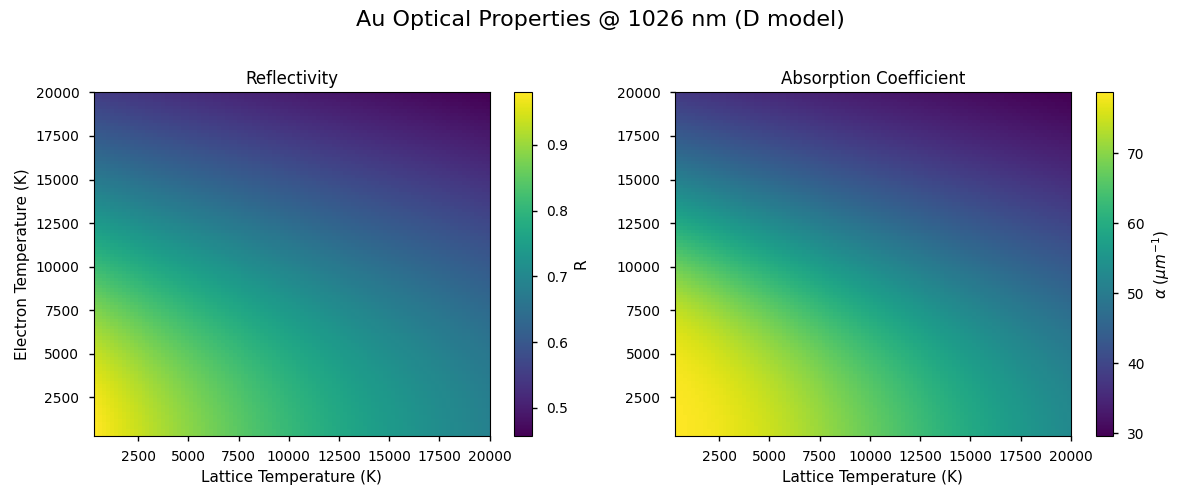
\includegraphics[width=\linewidth,height=5.28cm,keepaspectratio]{../thesis/figures/ch3/heatmaps_1026nm_D.png}
    \end{column}
    \begin{column}{0.29\textwidth}
      \centering
      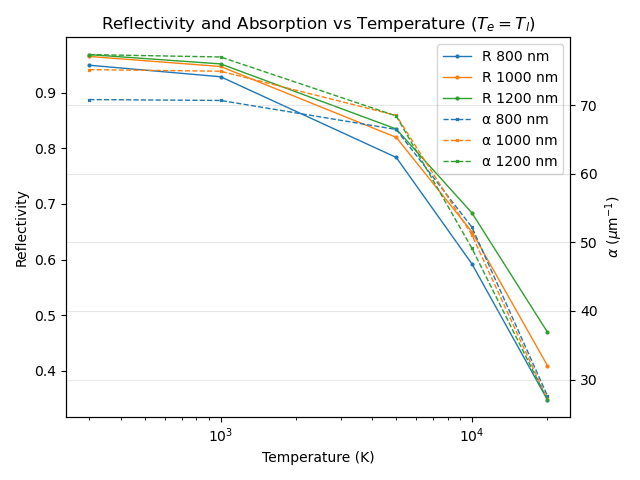
\includegraphics[width=\linewidth,height=2.85cm,keepaspectratio]{../thesis/figures/ch3/tempseries_multi_LD.png}\par
      \vspace{-0.03cm}
      \begin{beamercolorbox}[wd=\linewidth,sep=0.38em]{normal text}
        \scriptsize\textbf{\color{GVTeal}Evidence reading}\par
        \vspace{0.05cm}
        \tiny
        \(\bullet\) Au optical response is evaluated at the \(1026\,\mathrm{nm}\) operating wavelength.\par
        \vspace{0.05cm}
        \(\bullet\) Across the plotted thermal range, \(\alpha\) changes more strongly than \(R\).\par
        \vspace{0.05cm}
        \(\bullet\) The equal-temperature Lorentz--Drude series captures decreasing \(R\) and increasing attenuation with heating.
      \end{beamercolorbox}
    \end{column}
  \end{columns}
\end{frame}

\GVSetBackupSlide{A5}
\GVSetSource{Source: thesis Ch. 1, ballistic-electron figure and Table 1.8.}
\begin{frame}[t]{Ballistic transport and finite-film source corrections}
  \hypertarget{supp:physics-ballistic}{}
  \vspace{-0.18cm}\hfill
  \GVBackupSectionButton{supp:physics}{Physical}\hspace{0.10cm}\GVBackupIndexButton
  \vspace{0.02cm}
  \begin{columns}[T,totalwidth=0.95\textwidth]
    \begin{column}{0.28\textwidth}
      \centering
      \GVOmissionNotice{Original third-party/adapted figure omitted from public source pending redistribution rights.}
    \end{column}
    \begin{column}{0.28\textwidth}
      \small\textbf{\color{GVTeal}Table 1.8: \(\delta_b\) (nm)}\par
      \vspace{0.06cm}\centering\scriptsize
      \begin{tabular}{@{}lr@{\qquad}lr@{}}
        \rowcolor{GVTealTint}\textbf{Metal} & \textbf{nm} & \textbf{Metal} & \textbf{nm}\\
        Ag & 142 & Al & 46\\
        Au & 100 & Cr & 14\\
        Cu & 70 & Ni & 11\\
        Ti & 17.04\(^*\) & Steel & 0\(^{**}\)
      \end{tabular}\par
      \vspace{0.14cm}\scriptsize\color{GVSlate}
      \(^*\) optical-penetration estimate. \(^{**}\) value not supplied where optical data are unavailable.
    \end{column}
    \begin{column}{0.30\textwidth}
      \[
      \alpha'=\frac{1}{\delta_{\mathrm{opt}}+\delta_b}
      =\frac{\alpha}{1+\alpha\delta_b}
      \]
      \vspace{-0.28cm}
      \[
      b(L_z;\alpha')=\frac{1}{1-\exp(-\alpha'L_z)}
      \]
      \vspace{0.04cm}
      \begin{beamercolorbox}[wd=\linewidth,sep=0.40em]{normal text}
        \scriptsize
        \(\bullet\) Ballistic motion broadens the effective absorption depth.\par
        \vspace{0.11cm}
        \(\bullet\) Finite-film normalisation preserves deposited-energy accounting.\par
        \vspace{0.11cm}
        \(\bullet\) The correction matters when penetration/ballistic scales are not negligible relative to \(L_z\).
      \end{beamercolorbox}
    \end{column}
  \end{columns}
\end{frame}

\GVSetBackupSlide{A6a}
\GVSetSource{Sources: Lin et al. (2008); Fang et al. (2012). Conceptual synthesis; software-specific routes are not attributed to Fang.}
\begin{frame}[t]{Electronic-structure provenance of \(C_e(T_e)\) and \(G(T_e)\)}
  \hypertarget{supp:physics-ceg-provenance}{}
  \vspace{-0.18cm}\hfill
  \GVBackupSectionButton{supp:physics}{Physical}\hspace{0.10cm}\GVBackupIndexButton
  \vspace{0.04cm}
  \begin{center}
    \begin{tikzpicture}[
      >=stealth,
      base/.style={draw=GVSlate,fill=GVCanvas,rounded corners=2pt,align=center,font=\scriptsize,inner xsep=4pt,inner ysep=3pt,text width=3.05cm},
      ce/.style={base,draw=GVCapacityPurple,fill=GVCanvas},
      gg/.style={base,draw=GVCouplingOrange,fill=GVCanvas},
      result/.style={base,draw=GVTeal,fill=GVTealTint,font=\scriptsize\bfseries,text width=5.20cm},
      context/.style={base,draw=GVSlate,dashed,font=\scriptsize,text width=7.10cm}
    ]
      \node[base,text width=3.85cm] (dos) at (0,3.30) {Reference electronic DOS \(g(E)\)};
      \node[ce] (fd) at (-3.15,2.23) {Fermi--Dirac occupations};
      \node[ce] (mu) at (-3.15,1.43) {number constraint\\\(\mu(T_e)\)};
      \node[ce] (ue) at (-3.15,0.63) {\(U_e(T_e)\)\\\(C_e=\partial U_e/\partial T_e\)};
      \node[gg] (ep) at (3.15,2.23) {electron--phonon input\\or spectral moment};
      \node[gg] (weight) at (3.15,1.43) {DOS/Fermi-window weighting};
      \node[gg] (gt) at (3.15,0.63) {\(G(T_e)\)};
      \node[result] (curves) at (0,-0.18) {Reference thermophysical curves for nonlinear pTTM};
      \node[context] (generic) at (0,-0.94) {Generic context, not Fang-specific: phonons + e-ph matrices \(\rightarrow \alpha^2F,\lambda\langle\omega^2\rangle\)};
      \draw[->,line width=0.55pt,color=GVSlate] (dos.south west) -- (fd.north);
      \draw[->,line width=0.55pt,color=GVSlate] (dos.south east) -- (ep.north);
      \draw[->,line width=0.55pt,color=GVCapacityPurple] (fd) -- (mu);
      \draw[->,line width=0.55pt,color=GVCapacityPurple] (mu) -- (ue);
      \draw[->,line width=0.55pt,color=GVCapacityPurple] (ue) -- (curves);
      \draw[->,line width=0.55pt,color=GVCouplingOrange] (ep) -- (weight);
      \draw[->,line width=0.55pt,color=GVCouplingOrange] (weight) -- (gt);
      \draw[->,line width=0.55pt,color=GVCouplingOrange] (gt) -- (curves);
      \draw[->,densely dashed,line width=0.45pt,color=GVSlate] (generic.north east) to[out=35,in=-35] (gt.east);
    \end{tikzpicture}
  \end{center}
  \vspace{-0.08cm}
  \begin{beamercolorbox}[wd=0.96\textwidth,sep=0.24em]{normal text}
    \scriptsize\textbf{\color{GVTitleRed}Caveat.} Rigid-/frozen-DOS closures are approximate; Fang et al. report DOS/band-structure changes above \(T_e\approx10^4\,\mathrm K\).
  \end{beamercolorbox}
\end{frame}

\GVSetBackupSlide{A6b}
\GVSetSource{Source: thesis Chs. 1, 3, and 4; Fang\_2012; Lin\_2008.}
\begin{frame}[t]{From reference thermophysical curves to pTTM closures}
  \hypertarget{supp:physics-ceg-closures}{}
  \vspace{-0.18cm}\hfill
  \GVBackupSectionButton{supp:physics}{Physical}\hspace{0.10cm}\GVBackupIndexButton
  \vspace{0.03cm}
  \begin{columns}[T,totalwidth=0.94\textwidth]
    \begin{column}{0.43\textwidth}
      \begin{beamercolorbox}[wd=\linewidth,sep=0.52em]{normal text}
        \small\textbf{\color{GVCapacityPurple}Material-specific solver route}\par
        \vspace{0.10cm}
        \centering
        \begin{tikzpicture}[>=stealth,node distance=0.25cm,
          box/.style={draw=GVCapacityPurple,fill=GVCanvas,rounded corners=2pt,align=center,font=\scriptsize,minimum width=3.85cm,inner ysep=3pt}]
          \node[box] (r) {reference \(C_e(T_e),G(T_e)\) curves};
          \node[box,below=of r] (p) {low-/high-temperature\\piecewise polynomials};
          \node[box,below=of p] (s) {direct nonlinear pTTM closure};
          \draw[->,color=GVCapacityPurple,line width=0.55pt] (r) -- (p);
          \draw[->,color=GVCapacityPurple,line width=0.55pt] (p) -- (s);
        \end{tikzpicture}
      \end{beamercolorbox}
    \end{column}
    \begin{column}{0.43\textwidth}
      \begin{beamercolorbox}[wd=\linewidth,sep=0.52em]{normal text}
        \small\textbf{\color{GVTeal}Synthetic nonlinear-data route}\par
        \vspace{0.10cm}
        \centering
        \begin{tikzpicture}[>=stealth,node distance=0.25cm,
          box/.style={draw=GVTeal,fill=GVTealTint,rounded corners=2pt,align=center,font=\scriptsize,minimum width=3.85cm,inner ysep=3pt}]
          \node[box] (r) {reference \(C_e(T_e),G(T_e)\) curves};
          \node[box,below=of r] (b) {common fixed cubic\\log-B-spline basis};
          \node[box,below=of b] (c) {coefficient-envelope sampling\\\(\longrightarrow\) accepted positive curves};
          \draw[->,color=GVTeal,line width=0.55pt] (r) -- (b);
          \draw[->,color=GVTeal,line width=0.55pt] (b) -- (c);
        \end{tikzpicture}\par
        \vspace{0.05cm}\scriptsize\hyperlink{supp:sampling-spline-basis}{\color{GVTeal}\textbf{See D5: basis and knot convention.}}
      \end{beamercolorbox}
    \end{column}
  \end{columns}
  \vspace{0.13cm}
  \begin{columns}[T,totalwidth=0.94\textwidth]
    \begin{column}{0.58\textwidth}
      \centering\scriptsize
      \textbf{Chapter 3 fit convention}\par
      \vspace{0.04cm}
      \begin{tabular}{@{}lccc@{}}
        \rowcolor{black!10}\textbf{Metal} & \(T_{\mathrm{th}}\) (K) & \(C_e\) degrees & \(G\) degrees\\
        Au & 2500 & \((1,11)\) & \((0,15)\)\\
        Ag & 4250 & \((1,11)\) & \((0,15)\)\\
        Cu & 2250 & \((1,11)\) & \((0,15)\)\\
        Fe & 750 & \((1,12)\) & \((0,15)\)\\
        Ni & 500 & \((1,12)\) & \((2,15)\)\\
        Ti & 1000 & \((1,11)\) & \((2,15)\)
      \end{tabular}
    \end{column}
    \begin{column}{0.32\textwidth}
      \begin{beamercolorbox}[wd=\linewidth,sep=0.40em]{normal text}
        \scriptsize\textbf{\color{GVSlate}Provenance boundary}\par
        \vspace{0.05cm}
        \scriptsize Au curves: Fang et al. (2012).\par
        \vspace{0.05cm}
        \scriptsize Multi-metal first-principles context: Lin et al. (2008).\par
        \vspace{0.05cm}
        \scriptsize The checked non-Au packaged arrays contain no per-file source metadata.
      \end{beamercolorbox}
    \end{column}
  \end{columns}
\end{frame}

\GVSetBackupSlide{A7}
\GVSetSource{Source: thesis Ch. 3; Fang\_2012.}
\begin{frame}[t]{Full-range Au thermophysical fits}
  \hypertarget{supp:au-full-range}{}
  \vspace{-0.18cm}\hfill
  \GVBackupSectionButton{supp:physics}{Physical}\hspace{0.10cm}\GVBackupIndexButton
  \vspace{-0.06cm}
  \begin{center}
    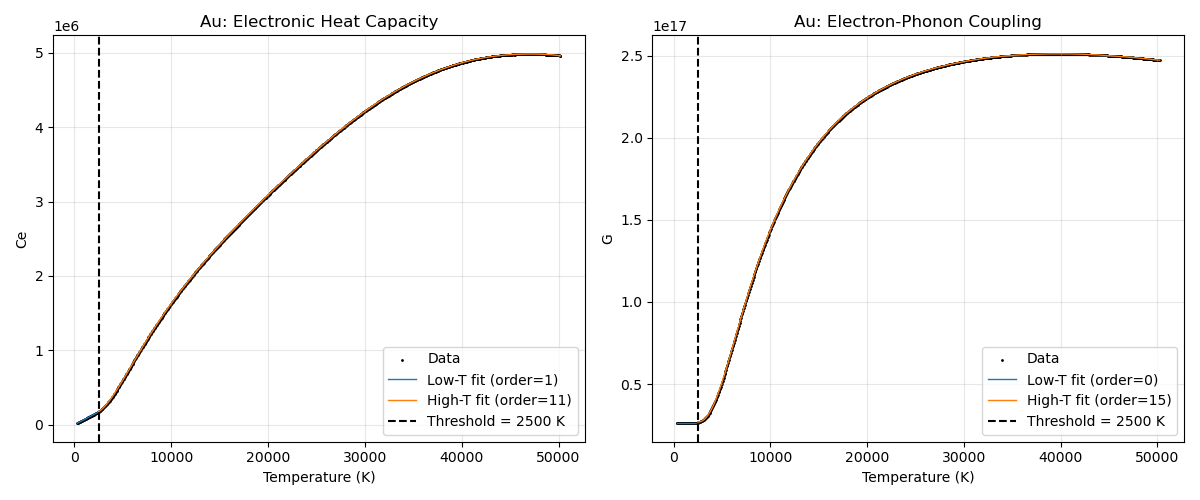
\includegraphics[width=0.92\textwidth]{../thesis/figures/ch3/Au_Ce_G_curves.png}
  \end{center}
\end{frame}

\GVSetBackupSlide{A8}
\GVSetSource{Source: thesis Ch. 3, Figure 3.8 and Table 3.3.}
\begin{frame}[t]{Ni thermophysical fitting evidence}
  \hypertarget{supp:physics-ni-fits}{}
  \vspace{-0.18cm}\hfill
  \GVBackupSectionButton{supp:physics}{Physical}\hspace{0.10cm}\GVBackupIndexButton
  \vspace{-0.03cm}
  \begin{columns}[T,totalwidth=0.95\textwidth]
    \begin{column}{0.61\textwidth}
      \centering
      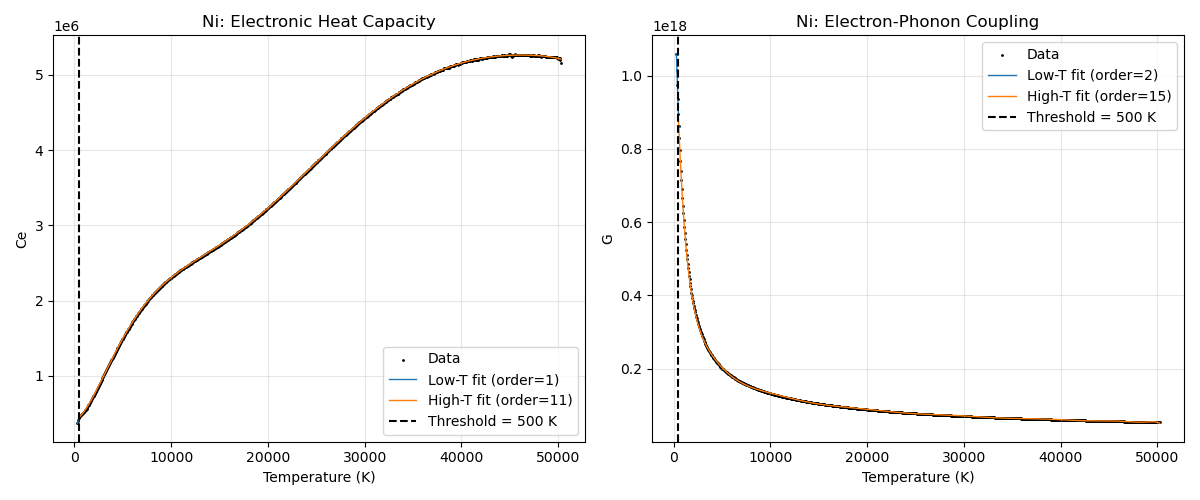
\includegraphics[width=\linewidth,height=5.48cm,keepaspectratio]{../thesis/figures/ch3/Ni_Ce_G_curves.png}
    \end{column}
    \begin{column}{0.28\textwidth}
      \begin{beamercolorbox}[wd=\linewidth,sep=0.46em]{normal text}
        \small\textbf{\color{GVCapacityPurple}Ni fit convention}\par
        \vspace{0.08cm}\scriptsize
        \begin{tabular}{@{}lr@{}}
          \rowcolor{GVTealTint}\textbf{Quantity} & \textbf{Value}\\
          \(T_{\mathrm{th}}\) & \(500\,\mathrm K\)\\
          \(C_e\) degrees & \((1,12)\)\\
          \(G\) degrees & \((2,15)\)
        \end{tabular}\par
        \vspace{0.13cm}
        \scriptsize Nickel requires a quadratic low-temperature \(G\) fit, unlike Au where the corresponding order is \((0,15)\); its \(C_e\) high-temperature order is also one degree higher.
      \end{beamercolorbox}
    \end{column}
  \end{columns}
\end{frame}

\GVSetBackupSlide{B0}
\GVSetSource{}
\begin{frame}[t]{B. Numerical methods and solver details}
  \hypertarget{supp:numerics}{}
  \vspace{-0.20cm}\hfill\GVBackupIndexButton
  \vspace{0.14cm}
  \begin{columns}[T,totalwidth=0.92\textwidth]
    \begin{column}{0.44\textwidth}
      \centering\GVBackupCard{supp:numerics-parameters}{B1 Dimensionless coefficients and simulation parameters}{Gold benchmark scales, physical constants, and retained 1D/2D numerical settings.}
      \vspace{0.18cm}
      \centering\GVBackupCard{supp:numerics-picard}{B4 Monolithic Picard and Anderson implementation}{Fixed-point loop, acceleration history, convergence test, and retained controls.}
    \end{column}
    \begin{column}{0.44\textwidth}
      \centering\GVBackupCard{supp:numerics-imex-stages}{B5 IMEX tableaux and stage equations}{Heun/CN additive pair, operator split, and compact nonlinear stage relations.}
      \vspace{0.18cm}
      \centering\GVBackupCard{supp:numerics-strong-gs}{B6 Strong Gauss--Seidel partitioned algorithm}{Electron-first/lattice-second sequencing and lower-triangular stage dependence.}
    \end{column}
  \end{columns}
\end{frame}

\GVSetBackupSlide{B1}
\GVSetSource{Source: thesis Ch. 2, Eqs. (2.5)--(2.6), Tables 2.1--2.2.}
\begin{frame}[t]{Dimensionless coefficients and simulation parameters}
  \hypertarget{supp:numerics-parameters}{}
  \vspace{-0.18cm}\hfill
  \GVBackupSectionButton{supp:numerics}{Numerics}\hspace{0.10cm}\GVBackupIndexButton
  \vspace{-0.05cm}
  \begin{center}
    \scriptsize
    \[
      \begin{aligned}
        &\underbrace{D_1(u)=\frac{t_{\mathrm{ref}}k_{e,0}}{L_{\mathrm{ref}}^2C_e(T_{\mathrm{ref}}u)},\quad
        K(u,v)=\frac{k_e(T_{\mathrm{ref}}u,T_{\mathrm{ref}}v)}{k_{e,0}},\quad
        D_2=\frac{t_{\mathrm{ref}}k_l}{L_{\mathrm{ref}}^2C_l}}_{\text{diffusion scales}}\\[-0.04cm]
        &\underbrace{c_1(u)=\frac{t_{\mathrm{ref}}G(T_{\mathrm{ref}}u)}{C_e(T_{\mathrm{ref}}u)},\quad
        c_2(u)=\frac{t_{\mathrm{ref}}G(T_{\mathrm{ref}}u)}{C_l},\quad
        s=\frac{t_{\mathrm{ref}}S_{\mathrm{dim}}}{T_{\mathrm{ref}}C_e(T_{\mathrm{ref}}u)}}_{\text{coupling and source scales}},\qquad
        S_{\mathrm{dim}}=S(t_{\mathrm{ref}}t,L_{\mathrm{ref}}\mathbf x;T_{\mathrm{ref}}u,T_{\mathrm{ref}}v).
      \end{aligned}
    \]
  \end{center}
  \vspace{-0.20cm}
  \begin{columns}[T,totalwidth=0.94\textwidth]
    \begin{column}{0.42\textwidth}
      \begin{beamercolorbox}[wd=\linewidth,sep=0.46em]{normal text}
        \small\textbf{\color{GVCapacityPurple}Retained Au physical constants}\par
        \vspace{0.07cm}
        \scriptsize
        \renewcommand{\arraystretch}{1.08}
        \begin{tabular}{@{}lr@{}}
          \rowcolor{GVTealTint}
          \textbf{Quantity} & \textbf{Value} \\
          \(T_R\) & \(300\,\mathrm{K}\) \\
          \(C_e(T_R)\) & \(2.04\times10^4\,\mathrm{J\,m^{-3}K^{-1}}\) \\
          \(C_l\) & \(2.5\times10^6\,\mathrm{J\,m^{-3}K^{-1}}\) \\
          \(G\) & \(2.1\times10^{16}\,\mathrm{W\,m^{-3}K^{-1}}\) \\
          \(k_{e,0}\) & \(318\,\mathrm{W\,m^{-1}K^{-1}}\) \\
          \(k_l\) & \(3.18\,\mathrm{W\,m^{-1}K^{-1}}\) \\
        \end{tabular}
      \end{beamercolorbox}
    \end{column}
    \begin{column}{0.48\textwidth}
      \begin{beamercolorbox}[wd=\linewidth,sep=0.46em]{normal text}
        \small\textbf{\color{GVTeal}Reference and benchmark settings}\par
        \vspace{0.07cm}
        \scriptsize
        \(t_{\mathrm{ref}}=\tau_p=10\,\mathrm{ps}\), \(L_{\mathrm{ref}}=L_z=1\,\mu\mathrm{m}\), and \(F^*=F/F_{\mathrm{ref}}\); \(T_{\mathrm{ref}}\) keeps \(u,v=\mathcal{O}(1)\).\par
        \vspace{0.08cm}
        \renewcommand{\arraystretch}{1.08}
        \begin{tabular}{@{}lcc@{}}
          \rowcolor{GVTealTint}
          \textbf{Setting} & \textbf{1D} & \textbf{2D} \\
          Evolution horizon & \multicolumn{2}{c}{\(100\,\mathrm{ps}\)} \\
          Benchmark fluence & \multicolumn{2}{c}{\(100\,\mathrm{J\,m^{-2}}\)} \\
          \(N_x\) / \(N_z\) & \(201\) / -- & \(101\) / \(101\) \\
          \(N_t\) & \(1001\) & \(201\) \\
          Width / \(R_0\) factor & -- & \(1\,\mu\mathrm{m}\) / \(4\) \\
        \end{tabular}
      \end{beamercolorbox}
    \end{column}
  \end{columns}
\end{frame}

\GVSetBackupSlide{B4}
\GVSetSource{Source: thesis Ch. 2, Algorithm 1, Table 2.4, Eqs. (2.33)--(2.34); Pollock\_2018.}
\begin{frame}[t]{Monolithic Picard iteration with Anderson acceleration}
  \hypertarget{supp:numerics-picard}{}
  \vspace{-0.18cm}\hfill
  \GVBackupSectionButton{supp:numerics}{Numerics}\hspace{0.10cm}\GVBackupIndexButton
  \vspace{0.05cm}
  \begin{columns}[T,totalwidth=0.94\textwidth]
    \begin{column}{0.56\textwidth}
      \begin{beamercolorbox}[wd=\linewidth,sep=0.54em]{normal text}
        \small\textbf{\color{GVTeal}Algorithm 1, condensed}\par
        \vspace{0.08cm}
        \scriptsize
        \textbf{1. Initialise.} \(\mathbf{x}^{(0)}=[(\mathbf u^n)^\top,(\mathbf v^n)^\top]^\top\), with empty state/residual histories.\par
        \textbf{2. Assemble and solve.} Evaluate \(\mathbf s^{(k)}\), assemble \(\mathbf b^{(k)}\), and solve \(\mathbf M\mathbf x_{\mathrm{raw}}^{(k+1)}=\mathbf b^{(k)}\).\par
        \textbf{3. Form residual.} \(\mathbf f^{(k)}=\mathbf x_{\mathrm{raw}}^{(k+1)}-\mathbf x^{(k)}\).\par
        \textbf{4. Anderson correction.} With history, build \(\Delta\mathbf F,\Delta\mathbf X\), solve the regularised least-squares problem, then set \(\mathbf x^{(k+1)}=\mathbf x_{\mathrm{raw}}^{(k+1)}-\Delta\mathbf X\boldsymbol\gamma\).\par
        \textbf{5. Test and retain history.} Stop when \(\|\mathbf x^{(k+1)}-\mathbf x^{(k)}\|_2/(\|\mathbf x^{(k)}\|_2+\epsilon_{\mathrm{tol}})<\tau_{\mathrm P}\); otherwise append FIFO history.
      \end{beamercolorbox}
      \vspace{0.12cm}
      \scriptsize
      \[
        (\Delta\mathbf F^\top\Delta\mathbf F+\epsilon\mathbf I)\boldsymbol\gamma
        =\Delta\mathbf F^\top\mathbf f^{(k)}.
      \]
      \vspace{-0.12cm}
      \scriptsize\color{GVSlate}For the retained \(\beta=1\), the relaxed Anderson update reduces to the displayed form.
    \end{column}
    \begin{column}{0.34\textwidth}
      \begin{beamercolorbox}[wd=\linewidth,sep=0.54em]{normal text}
        \small\textbf{\color{GVCouplingOrange}Retained controls}\par
        \vspace{0.08cm}
        \scriptsize
        \renewcommand{\arraystretch}{1.13}
        \begin{tabular}{@{}ll@{}}
          \rowcolor{GVTealTint}
          \textbf{Control} & \textbf{Value} \\
          \(k_{\max}\) & \(30\) \\
          \(\tau_{\mathrm P}\) & \(10^{-6}\) \\
          \(m\) & \(5\) \\
          \(\beta\) & \(1.0\) \\
          \(\epsilon_{\mathrm{tol}}\) & \(10^{-16}\) \\
          \(\epsilon\) & \(10^{-8}\) \\
        \end{tabular}\par
        \vspace{0.10cm}
        \color{GVSlate}\(m\): history depth; \(\tau_{\mathrm P}\): convergence tolerance; \(\epsilon\): regularisation; \(\beta=1\): full relaxation.
      \end{beamercolorbox}
    \end{column}
  \end{columns}
\end{frame}

\GVSetBackupSlide{B5}
\GVSetSource{Source: thesis Ch. 2, Table 2.5 and nonlinear IMEX stage equations; Kennedy\_2003; Ascher\_1997.}
\begin{frame}[t]{Heun--Crank--Nicolson IMEX stages}
  \hypertarget{supp:numerics-imex-stages}{}
  \vspace{-0.18cm}\hfill
  \GVBackupSectionButton{supp:numerics}{Numerics}\hspace{0.10cm}\GVBackupIndexButton
  \vspace{0.02cm}
  \begin{columns}[T,totalwidth=0.96\textwidth]
    \begin{column}{0.36\textwidth}
      \begin{beamercolorbox}[wd=\linewidth,sep=0.50em]{normal text}
        \small\textbf{\color{GVSourceBlue}Explicit Heun}\hfill\textbf{\color{GVDiffusionGreen}Implicit CN}\par
        \vspace{0.10cm}
        \centering\scriptsize
        \begin{minipage}[t]{0.42\linewidth}
          \centering
          \(\begin{array}{c|cc}
            0 & 0 & 0\\
            1 & 1 & 0\\ \hline
              & \tfrac12 & \tfrac12
          \end{array}\)
        \end{minipage}\hfill
        \begin{minipage}[t]{0.42\linewidth}
          \centering
          \(\begin{array}{c|cc}
            0 & 0 & 0\\
            1 & \tfrac12 & \tfrac12\\ \hline
              & \tfrac12 & \tfrac12
          \end{array}\)
        \end{minipage}\par
        \vspace{0.13cm}
        \scriptsize\color{GVSlate}
        \textbf{ARK2(1)2[2]SA:} two stages, second order, embedded first order, stiffly accurate implicit tableau.
      \end{beamercolorbox}
    \end{column}
    \begin{column}{0.58\textwidth}
      \begin{beamercolorbox}[wd=\linewidth,sep=0.50em]{normal text}
        \small\textbf{\color{GVTeal}Additive split}\par
        \vspace{-0.08cm}
        \scriptsize
        \[
          \mathbf F(\boldsymbol\theta,t)=
          \underbrace{\textcolor{GVDiffusionGreen}{\mathbf L(\boldsymbol\theta)[\boldsymbol\theta]}+
          \textcolor{GVCouplingOrange}{\mathbf C(\boldsymbol\theta)[\boldsymbol\theta]}}_{\mathbf g\ \text{implicit}}
          +\underbrace{\textcolor{GVSourceBlue}{\mathbf S(t,\boldsymbol\theta)}}_{\mathbf f\ \text{explicit}}.
        \]
      \end{beamercolorbox}
      \vspace{0.07cm}
      \begin{beamercolorbox}[wd=\linewidth,sep=0.36em]{normal text}
        \small\textbf{\color{GVSourceBlue}Stage 1}\hfill\scriptsize\color{GVSlate}initial evaluation at \(t_n\)\par
        \vspace{-0.08cm}
        \scriptsize
        \[
          \boldsymbol\theta_{n,1}=\boldsymbol\theta^n,\qquad
          \widehat{\mathbf k}_{n,1}
          =\Delta_t\mathbf f(\boldsymbol\theta_{n,1},t_n),
          \qquad
          \mathbf k_{n,1}
          =\Delta_t\mathbf g(\boldsymbol\theta_{n,1},t_n).
        \]
      \end{beamercolorbox}
      \vspace{0.07cm}
      \begin{beamercolorbox}[wd=\linewidth,sep=0.36em]{normal text}
        \small\textbf{\color{GVDiffusionGreen}Stage 2}\hfill\scriptsize\color{GVSlate}Crank--Nicolson implicit correction at \(t_{n+1}\)\par
        \vspace{-0.08cm}
        \scriptsize
        \[
          \boldsymbol\theta_{n,2}
          =
          \boldsymbol\theta^n
          +\widehat{\mathbf k}_{n,1}
          +\tfrac12\mathbf k_{n,1}
          +\tfrac12\mathbf k_{n,2},
          \qquad
          \mathbf k_{n,2}
          =
          \Delta_t\mathbf g(\boldsymbol\theta_{n,2},t_{n+1}).
        \]
        \vspace{-0.08cm}
        {\scriptsize\color{GVSlate}
        2D nonlinear implementation: \(M=N_xN_z\) unknowns per thermal field.\par
        \vspace{0.03cm}
        The strong predictor supplies the stage coupling data.}
      \end{beamercolorbox}
    \end{column}
  \end{columns}
\end{frame}

\GVSetBackupSlide{B6}
\GVSetSource{Source: thesis Ch. 2, Algorithm 2; Huang\_2019.}
\begin{frame}[t]{Strong Gauss--Seidel partitioned IMEX update}
  \hypertarget{supp:numerics-strong-gs}{}
  \vspace{-0.18cm}\hfill
  \GVBackupSectionButton{supp:numerics}{Numerics}\hspace{0.10cm}\GVBackupIndexButton
  \vspace{-0.10cm}
  \begin{columns}[T,totalwidth=0.94\textwidth]
    \begin{column}{0.48\textwidth}
      \begin{beamercolorbox}[wd=\linewidth,sep=0.52em]{normal text}
        \small\textbf{\color{GVTeal}Algorithm 2, retained partitioned stage update}\par
        \vspace{0.08cm}
        \scriptsize
        \textbf{Specialised pTTM stage solve:}\par
        \textbf{1. Electron first.} Solve for \(\mathbf u_*^n\) with the predictor \(\tilde{\mathbf c}^{\,e}=\mathbf c(\mathbf u_*^n,\mathbf v^n)\); evaluate the explicit source contribution and solve the implicit diffusion--coupling stage.\par
        \vspace{0.12cm}
        \textbf{2. Lattice second.} Solve for \(\mathbf v_*^n\) with \(\tilde{\mathbf c}^{\,l}=\mathbf c(\mathbf u_*^n,\mathbf v_*^n)\); solve the implicit lattice diffusion--coupling stage using the updated electron stage field.\par
        \vspace{0.12cm}
        \textbf{3. Time update.} Combine the old-time and converged stage residuals to obtain \((\mathbf u^{n+1},\mathbf v^{n+1})\).
      \end{beamercolorbox}
      \vspace{0.08cm}
      \begin{beamercolorbox}[wd=\linewidth,sep=0.38em]{normal text}
        \scriptsize
        Retained split: \textcolor{GVDiffusionGreen}{implicit diffusion} + \textcolor{GVCouplingOrange}{implicit coupling}; \textcolor{GVSourceBlue}{explicit source}.\par
        Each nonlinear implicit stage uses the B4 Picard--Anderson loop.
      \end{beamercolorbox}
    \end{column}
    \begin{column}{0.42\textwidth}
      \centering
      \begin{tikzpicture}[>=stealth, node distance=0.68cm and 0.42cm]
        \node[draw=GVDiffusionGreen,fill=GVTealTint,rounded corners=2pt,align=center,font=\small,minimum width=3.45cm,minimum height=1.00cm] (e) {electron stage\\\(\mathbf u_*^n\mid\mathbf v^n\)};
        \node[draw=GVCouplingOrange,fill=GVTealTint,rounded corners=2pt,align=center,font=\small,minimum width=3.45cm,minimum height=1.00cm,below=of e] (l) {lattice stage\\\(\mathbf v_*^n\mid\mathbf u_*^n\)};
        \node[draw=GVCapacityPurple,fill=GVCanvas,rounded corners=2pt,align=center,font=\footnotesize,minimum width=3.45cm,minimum height=0.62cm,below=0.32cm of l] (pa) {nonlinear stage solve\\Picard + Anderson};
        \draw[->,line width=1.35pt,color=GVCouplingOrange] (e) -- node[right=0.18cm,font=\footnotesize,color=GVSlate,align=left,fill=white,inner sep=1pt] {updated\\\(\mathbf u_*^n\)} (l);
        \draw[->,densely dashed,color=GVSlate,thick] ([xshift=-1.75cm]e.west) -- node[above,font=\footnotesize,color=GVSlate] {lagged \(\mathbf v^n\)} (e.west);
        \draw[->,thick,color=GVCapacityPurple] (l) -- (pa);
      \end{tikzpicture}\par
      \vspace{0.16cm}
      \scriptsize\textbf{\color{GVCapacityPurple}Stage-solve Jacobian}\par
      \vspace{-0.14cm}
      \[
        \begin{bmatrix}
          \partial_{\mathbf u_*}\mathbf r^e & 0\\
          \partial_{\mathbf u_*}\mathbf r^l & \partial_{\mathbf v_*}\mathbf r^l
        \end{bmatrix}
      \]
      \vspace{-0.16cm}
      \scriptsize\color{GVSlate}Lower-triangular current-stage dependence.
    \end{column}
  \end{columns}
\end{frame}

\GVSetBackupSlide{C0}
\GVSetSource{}
\begin{frame}[t]{Threshold-search procedures}
  \hypertarget{supp:threshold}{}
  \vspace{-0.20cm}\hfill\GVBackupIndexButton
  \vspace{0.14cm}
  \begin{columns}[T,totalwidth=0.92\textwidth]
    \begin{column}{0.44\textwidth}
      \centering\GVBackupCard{supp:threshold-direct-search}{C1 Direct exponential bracketing and bisection}{Two-stage direct pTTM threshold search and its thermal crossing criterion.}
      \vspace{0.18cm}
      \centering\GVBackupCard{supp:threshold-direct-results}{C3 Direct pTTM threshold evidence}{Selected Chapter 3 linear and nonlinear 2D threshold benchmarks.}
    \end{column}
    \begin{column}{0.44\textwidth}
      \centering\GVBackupCard{supp:threshold-controls}{C2 Search controls and stopping criteria}{Retained fluence limits, iteration controls, and certified bracket-width termination.}
      \vspace{0.18cm}
      \centering\GVBackupCard{supp:threshold-surrogate-inversion}{C4 Surrogate response-curve inversion}{First crossing on a predicted response curve with log-fluence interpolation.}
    \end{column}
  \end{columns}
\end{frame}

\GVSetBackupSlide{C1}
\GVSetSource{Source: thesis Ch. 3, Fig. 3.9; Appendix B.}
\begin{frame}[t]{Direct threshold search: exponential bracketing and bisection}
  \hypertarget{supp:threshold-direct-search}{}
  \vspace{-0.18cm}\hfill
  \GVBackupSectionButton{supp:threshold}{Threshold}\hspace{0.10cm}\GVBackupIndexButton
  \vspace{-0.06cm}
  \begin{columns}[T,totalwidth=0.94\textwidth]
    \begin{column}{0.33\textwidth}
      \small\textbf{\color{GVCouplingOrange}Thermal crossing criterion}\par
      \vspace{0.08cm}
      \[
        \begin{aligned}
          \phi(F)&=T_{l,\max}(F)-T_m,\\[-0.08cm]
          \phi(F_{\mathrm{th}})&=0.
        \end{aligned}
      \]
      \vspace{0.04cm}
      \begin{beamercolorbox}[wd=\linewidth,sep=0.48em]{normal text}
        \small\textbf{\color{GVSourceBlue}Two-stage procedure}\par
        \vspace{0.10cm}
        \scriptsize
        \textbf{1. Exponential expansion}\par
        Increase \(F\) multiplicatively until the thermal crossing is bracketed.\par
        \vspace{0.15cm}
        \textbf{2. Bisection refinement}\par
        Contract the bracket to the requested fluence tolerance.
      \end{beamercolorbox}
      \vspace{0.08cm}
      \scriptsize\color{GVSlate}
      Each evaluation of \(\phi(F)\) is one transient pTTM solve.
    \end{column}
    \begin{column}{0.57\textwidth}
      \centering
      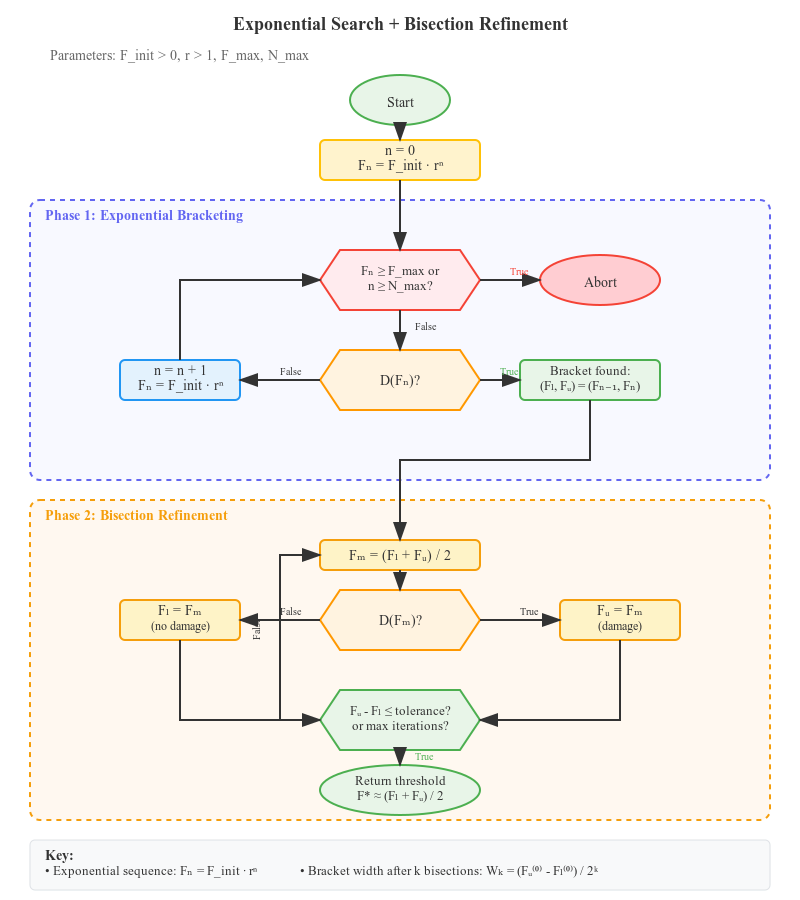
\includegraphics[height=5.00cm,keepaspectratio]{../thesis/figures/ch3/exponential_bisection_flowchart.png}
    \end{column}
  \end{columns}
  \vspace{-0.08cm}
\end{frame}

\GVSetBackupSlide{C2}
\GVSetSource{Source: thesis Ch. 3, Table 3.5; Appendix B.}
\begin{frame}[t]{Threshold-search controls and stopping criteria}
  \hypertarget{supp:threshold-controls}{}
  \vspace{-0.18cm}\noindent\hfill
  \GVBackupSectionButton{supp:threshold}{Threshold}\hspace{0.08cm}\GVBackupIndexButton\par
  \vspace{0.13cm}
  \begin{columns}[T,totalwidth=0.94\textwidth]
    \begin{column}{0.52\textwidth}
      \begin{beamercolorbox}[wd=\linewidth,sep=0.55em]{normal text}
        \small\textbf{\color{GVTeal}Common search controls}\par
        \vspace{0.10cm}
        \scriptsize
        \renewcommand{\arraystretch}{1.16}
        \begin{tabular}{@{}ll@{}}
          \rowcolor{GVTealTint}
          \textbf{Control} & \textbf{Retained value} \\
          \(r\) & \(2.0\) multiplicative expansion factor \\
          \(F_{\max}\) & \(10^{6}\,\mathrm{J\,m^{-2}}\) \\
          \(N_{\exp,\max}\) & \(30\) expansion iterations \\
          \(\varepsilon_F\) & \(0.5\,\mathrm{J\,m^{-2}}\) bisection tolerance \\
          \(N_{\mathrm{bis},\max}\) & \(20\) bisection iterations \\
          \(w_h\) & \(2.0\) pulse-duration half-window multiplier \\
        \end{tabular}
      \end{beamercolorbox}
    \end{column}
    \begin{column}{0.37\textwidth}
      \scriptsize
      \textbf{\color{GVCapacityPurple}Example initial fluences, selected runs}\par
      \vspace{0.06cm}
      Au \(2500\), Ni \(500\), Cu \(3750\) \(\mathrm{J\,m^{-2}}\).\par
      \color{GVSlate}Material-specific initial guesses, not universal defaults.\par
      \vspace{0.18cm}
      \small\textbf{\color{GVCouplingOrange}Damage predicate}\par
      \vspace{0.05cm}
      \centering\(T_{l,\max}(F)\geq T_m.\)\par
      \raggedright\scriptsize\color{GVSlate}Assumes a non-decreasing thermal response in fluence.\par
      \vspace{0.18cm}
      \small\textbf{\color{GVSourceBlue}Termination}\par
      \vspace{0.05cm}
      \centering\(F_b-F_a\leq\varepsilon_F.\)\par
      \raggedright\scriptsize\color{GVSlate}Report the final midpoint; its bracket half-width is the algorithmic enclosure.
    \end{column}
  \end{columns}
\end{frame}

\GVSetBackupSlide{C3}
\GVSetSource{Source: thesis Ch. 3, Tables 3.8--3.9.}
\begin{frame}[t]{Direct pTTM threshold estimates}
  \hypertarget{supp:threshold-direct-results}{}
  \vspace{-0.18cm}\hfill
  \GVBackupSectionButton{supp:threshold}{Threshold}\hspace{0.10cm}\GVBackupIndexButton
  \vspace{0.12cm}
  \begin{center}
    \begin{beamercolorbox}[wd=0.92\textwidth,sep=0.52em,center]{normal text}
      \small\color{GVSlate}
      Selected Chapter 3 two-dimensional single-pulse benchmarks: \(N_x=N_z=101\), \(N_t=501\), \(\tau_p=10\,\mathrm{ps}\), and \(\lambda_L=1030\,\mathrm{nm}\).
    \end{beamercolorbox}
  \end{center}
  \vspace{0.12cm}
  \begin{center}
    \small
    \renewcommand{\arraystretch}{1.36}
    \begin{tabular}{@{}lrrr@{}}
      \rowcolor{GVTealTint}
      \textbf{Material} & \textbf{Linear 2D} & \textbf{Nonlinear 2D} & \textbf{Common terminal \(\delta F_{\mathrm{bis}}\)} \\
      & \multicolumn{2}{c}{\(\hat F_{\mathrm{th}}\;[\mathrm{J\,m^{-2}}]\)} & \(\mathrm{J\,m^{-2}}\) \\
      \hline
      Au & 5867.00 & 11367.50 & 0.15 \\
      Ni & 990.23 & 1268.07 & 0.24 \\
      Cu & 8976.75 & 14311.06 & 0.23 \\
    \end{tabular}
  \end{center}
  \vspace{0.01cm}
  \begin{beamercolorbox}[wd=0.92\textwidth,sep=0.43em]{normal text}
    \scriptsize
    \textbf{\color{GVTitleRed}Configuration caveat.} The terminal width shown is the same in the corresponding 2D linear and nonlinear rows. Chapter 3 direct-solver benchmarks and the Chapter 4 high-grid/material comparisons use different evaluation configurations; their values are related but not interchangeable. Titanium is not a Table 3.8/3.9 case.
  \end{beamercolorbox}
  \vspace{-0.08cm}
\end{frame}

\GVSetBackupSlide{C4}
\GVSetSource{Source: thesis Ch. 4, Eqs. (4.11)--(4.13), Algorithm 5.}
\begin{frame}[t]{Surrogate threshold extraction from response curves}
  \hypertarget{supp:threshold-surrogate-inversion}{}
  \vspace{-0.18cm}\hfill
  \GVBackupSectionButton{supp:threshold}{Threshold}\hspace{0.10cm}\GVBackupIndexButton
  \vspace{0.04cm}
  \begin{center}
    \normalsize
    \[
      \log_{10}F_{\mathrm{th}}
      =
      \log_{10}F_a
      +
      \frac{T_m-\widehat T_a}{\widehat T_b-\widehat T_a}
      \left(\log_{10}F_b-\log_{10}F_a\right).
    \]
  \end{center}
  \vspace{-0.18cm}
  \begin{columns}[T,totalwidth=0.94\textwidth]
    \begin{column}{0.48\textwidth}
      \begin{beamercolorbox}[wd=\linewidth,sep=0.60em]{normal text}
        \small\textbf{\color{GVTeal}Algorithm 5, condensed}\par
        \vspace{0.10cm}
        \scriptsize
        \textbf{1.} Sort predictions by increasing fluence.\par
        \textbf{2.} Locate the first pair with \(\widehat T_{l,\max}(F_a)<T_m\leq\widehat T_{l,\max}(F_b)\).\par
        \textbf{3.} Interpolate in \(\log_{10}F\) between the bracket endpoints.\par
        \textbf{4.} Return no crossing when the sampled interval does not bracket \(T_m\).
      \end{beamercolorbox}
      \vspace{0.16cm}
      \begin{beamercolorbox}[wd=\linewidth,sep=0.54em]{normal text}
        \scriptsize
        \textbf{\color{GVCouplingOrange}Direct solver:} adaptive bracketing + bisection.\par
        \textbf{\color{GVSourceBlue}Surrogate curve:} first crossing + log-fluence interpolation.
      \end{beamercolorbox}
    \end{column}
    \begin{column}{0.40\textwidth}
      \centering
      \begin{tikzpicture}[>=stealth,x=0.77cm,y=0.68cm]
        \draw[->,color=GVCharcoal,line width=0.45pt] (0,0) -- (4.55,0) node[right,font=\scriptsize] {\(\log_{10}F\)};
        \draw[->,color=GVCharcoal,line width=0.45pt] (0,0) -- (0,3.55) node[above,font=\scriptsize,align=center] {\(\widehat T_{l,\max}\)};
        \draw[very thick,color=GVTeal] plot[smooth] coordinates {(0.30,0.36) (1.15,0.68) (1.95,1.16) (2.72,1.80) (3.38,2.42) (4.15,3.18)};
        \draw[densely dashed,color=GVTitleRed,line width=0.55pt] (0,1.80) -- (4.25,1.80) node[right,font=\scriptsize] {\(T_m\)};
        \fill[color=GVSourceBlue] (1.95,1.16) circle (1.6pt) node[below,font=\scriptsize] {\(F_a\)};
        \fill[color=GVSourceBlue] (2.72,1.80) circle (1.6pt) node[above right,font=\scriptsize] {\(F_b\)};
        \draw[densely dashed,color=GVCouplingOrange,line width=0.55pt] (2.72,0) -- (2.72,1.80);
        \node[font=\scriptsize,color=GVCouplingOrange,below] at (2.72,0) {\(F_{\mathrm{th}}\)};
      \end{tikzpicture}
    \end{column}
  \end{columns}
\end{frame}

\GVSetBackupSlide{D0}
\GVSetSource{}
\begin{frame}[t]{D. Dataset generation and sampling diagnostics}
  \hypertarget{supp:sampling}{}
  \vspace{-0.20cm}\hfill\GVBackupIndexButton
  \vspace{0.12cm}
  \begin{columns}[T,totalwidth=0.94\textwidth]
    \begin{column}{0.29\textwidth}
      \centering\GVBackupCard{supp:sampling-linear-ranges}{D1 Linear sampled variables and ranges}{Complete linear LHS support with deck notation and transforms.}
      \vspace{0.16cm}
      \centering\GVBackupCard{supp:sampling-spline-basis}{D5 Fixed cubic B-spline basis and knots}{Open-clamped basis, user knots, and coefficient convention.}
    \end{column}
    \begin{column}{0.29\textwidth}
      \centering\GVBackupCard{supp:sampling-nonlinear-scalars}{D2a Nonlinear scalar and transport ranges}{Independent scalar inputs and derived solver quantities.}
      \vspace{0.16cm}
      \centering\GVBackupCard{supp:sampling-feature-definitions}{D8a Final nonlinear 33-feature representation}{Exact final regression columns and analytical source-term-informed features.}
    \end{column}
    \begin{column}{0.29\textwidth}
      \centering\GVBackupCard{supp:sampling-nonlinear-optics}{D2b Nonlinear Lorentz--Drude ranges}{Grouped optical descriptors and the conditional sixth oscillator.}
      \vspace{0.16cm}
      \centering\GVBackupCard{supp:sampling-feature-correlation}{D8b Compact selected-feature correlation diagnostic}{16 selected features plus target, deck notation, and non-causal interpretation.}
    \end{column}
  \end{columns}
\end{frame}

\GVSetBackupSlide{D1}
\GVSetSource{Source: thesis Ch. 4, Table 4.1; linear feature-range report.}
\begin{frame}[t]{Linear pTTM sampled variables and ranges}
  \hypertarget{supp:sampling-linear-ranges}{}
  \vspace{-0.18cm}\hfill
  \GVBackupSectionButton{supp:sampling}{Sampling}\hspace{0.10cm}\GVBackupIndexButton
  \vspace{0.02cm}
  \begin{columns}[T,totalwidth=0.94\textwidth]
    \begin{column}{0.45\textwidth}
      \begin{beamercolorbox}[wd=\linewidth,sep=0.45em]{normal text}
        \small\textbf{\color{GVTeal}Thermal and transport variables}\par
        \vspace{0.07cm}
        \scriptsize\renewcommand{\arraystretch}{1.12}
        \begin{tabular}{@{}lll@{}}
          \rowcolor{GVTealTint}
          \textbf{Var.} & \textbf{Bounds and units} & \textbf{LHS} \\
          \(F\) & \([10,4\times10^4]\,\mathrm{J\,m^{-2}}\) & log \\
          \(C_e\) & \([10^4,2\times10^6]\,\mathrm{J\,m^{-3}K^{-1}}\) & log \\
          \(C_l\) & \([1.5,5]\times10^6\,\mathrm{J\,m^{-3}K^{-1}}\) & linear \\
          \(G\) & \([10^{16},5\times10^{18}]\,\mathrm{W\,m^{-3}K^{-1}}\) & log \\
          \(k_{e0}\) & \([20,500]\,\mathrm{W\,m^{-1}K^{-1}}\) & log \\
        \end{tabular}
      \end{beamercolorbox}
    \end{column}
    \begin{column}{0.45\textwidth}
      \begin{beamercolorbox}[wd=\linewidth,sep=0.45em]{normal text}
        \small\textbf{\color{GVCapacityPurple}Geometric and optical variables}\par
        \vspace{0.07cm}
        \scriptsize\renewcommand{\arraystretch}{1.12}
        \begin{tabular}{@{}lll@{}}
          \rowcolor{GVTealTint}
          \textbf{Var.} & \textbf{Bounds and units} & \textbf{LHS} \\
          \(\delta_b\) & \([10^{-9},1.5\times10^{-7}]\,\mathrm{m}\) & log \\
          \(\alpha\) & \([10^7,5\times10^8]\,\mathrm{m^{-1}}\) & log \\
          \(R\) & \([0.5,0.999]\) & linear \\
          \(\lambda\) & \([1000,1400]\,\mathrm{nm}\) & linear \\
          \(L_z\) & \([2\times10^{-7},10^{-6}]\,\mathrm{m}\) & log \\
        \end{tabular}
      \end{beamercolorbox}
    \end{column}
  \end{columns}
  \vspace{0.14cm}
  \begin{beamercolorbox}[wd=0.92\textwidth,sep=0.48em]{normal text}
    \scriptsize
    These ten sampled variables are also the linear regression features. \(k_l=0.01\,k_{e0}\) is derived; \(\tau_p=10\,\mathrm{ps}\) is fixed. LHS is performed in a unit cube and transformed linearly or in \(\log_{10}\) space on the \(101\times101\times501\) generation grid.
  \end{beamercolorbox}
\end{frame}

\GVSetBackupSlide{D2a}
\GVSetSource{Source: Ch. 4 Eq. (4.14); nonlinear range report.}
\begin{frame}[t]{Nonlinear scalar and transport sampling ranges}
  \hypertarget{supp:sampling-nonlinear-scalars}{}
  \vspace{-0.18cm}\hfill
  \GVBackupSectionButton{supp:sampling}{Sampling}\hspace{0.10cm}\GVBackupIndexButton
  \vspace{0.02cm}
  \begin{columns}[T,totalwidth=0.94\textwidth]
    \begin{column}{0.45\textwidth}
      \begin{beamercolorbox}[wd=\linewidth,sep=0.45em]{normal text}
        \small\textbf{\color{GVTeal}Thermal and conductivity inputs}\par
        \vspace{0.07cm}
        \scriptsize\renewcommand{\arraystretch}{1.15}
        \begin{tabular}{@{}lll@{}}
          \rowcolor{GVTealTint}
          \textbf{Var.} & \textbf{Bounds and units} & \textbf{Draw} \\
          \(F\) & \([10,4\times10^4]\,\mathrm{J\,m^{-2}}\) & log-U \\
          \(k_{e0}\) & \([20,500]\,\mathrm{W\,m^{-1}K^{-1}}\) & log-U \\
          \(C_l\) & \([1.5,5]\times10^6\,\mathrm{J\,m^{-3}K^{-1}}\) & U \\
          \(A_e\) & \([2.95\times10^6,2.56\times10^7]\,\mathrm{s^{-1}K^{-2}}\) & log-U \\
        \end{tabular}
      \end{beamercolorbox}
    \end{column}
    \begin{column}{0.45\textwidth}
      \begin{beamercolorbox}[wd=\linewidth,sep=0.45em]{normal text}
        \small\textbf{\color{GVDiffusionGreen}Scattering and geometric inputs}\par
        \vspace{0.07cm}
        \scriptsize\renewcommand{\arraystretch}{1.15}
        \begin{tabular}{@{}lll@{}}
          \rowcolor{GVTealTint}
          \textbf{Var.} & \textbf{Bounds and units} & \textbf{Draw} \\
          \(B_L\) & \([5.1\times10^{10},3.0\times10^{11}]\,\mathrm{s^{-1}K^{-1}}\) & log-U \\
          \(\delta_b\) & \([10^{-9},1.5\times10^{-7}]\,\mathrm{m}\) & log-U \\
          \(L_z\) & \([2\times10^{-7},10^{-6}]\,\mathrm{m}\) & log-U \\
          \(\lambda\) & \([1000,1400]\,\mathrm{nm}\) & U \\
        \end{tabular}
      \end{beamercolorbox}
    \end{column}
  \end{columns}
  \vspace{0.14cm}
  \begin{beamercolorbox}[wd=0.92\textwidth,sep=0.48em]{normal text}
    \scriptsize\textbf{\color{GVCapacityPurple}Derived, not independently sampled:}\quad
    \(k_l=0.01\,k_e(300\,\mathrm K,300\,\mathrm K)\); \(R\) and \(\alpha\) are Lorentz--Drude outputs; \(C_e(T_e)\) and \(G(T_e)\) are reconstructed from sampled spline coefficients. \(\mathrm{log\text{-}U}\) denotes log-uniform; \(\mathrm U\) denotes uniform.
  \end{beamercolorbox}
\end{frame}

\GVSetBackupSlide{D2b}
\GVSetSource{Source: nonlinear pTTM generation-range report; thesis Ch. 4.}
\begin{frame}[t]{Nonlinear Lorentz--Drude descriptor ranges}
  \hypertarget{supp:sampling-nonlinear-optics}{}
  \vspace{-0.18cm}\hfill
  \GVBackupSectionButton{supp:sampling}{Sampling}\hspace{0.10cm}\GVBackupIndexButton
  \vspace{0.01cm}
  \begin{beamercolorbox}[wd=0.92\textwidth,sep=0.42em]{normal text}
    \small\textbf{\color{GVTeal}Plasma descriptor}\quad
    \(\omega_p\in[5.5377\times10^{15},3.6280\times10^{16}]\,\mathrm{rad\,s^{-1}}\), sampled log-uniformly.
  \end{beamercolorbox}
  \vspace{0.10cm}
  \begin{center}
    \scriptsize\renewcommand{\arraystretch}{1.16}
    \begin{tabular}{@{}clll@{}}
      \rowcolor{GVTealTint}
      \textbf{Oscillator} & \textbf{Strength \(f_i\)} & \textbf{Damping \(\gamma_i\), eV} & \textbf{Resonance \(\Omega_i\), eV} \\
      \(0\) Drude & \([0.048,1.2675]\), log & \([0.015,0.123]\), log & \(0\), fixed \\
      \(1\) & \([0.012,1.3485]\), log & \([0.1205,6.7665]\), log & \([0.087,1.224]\), log \\
      \(2\) & \([0.005,0.5895]\), log & \([0.1725,3.777]\), log & \([0.291,6.7215]\), log \\
      \(3\) & \([0.0055,1.0845]\), log & \([0.0325,4.8195]\), log & \([0.7985,12.2775]\), log \\
      \(4\) & \([0.0005,1.26]\), log & \([0.458,9.438]\), log & \([0.9715,16.77]\), log \\
      \(5\) conditional & \([2.192,8.469]\), log & \([1.107,3.6285]\), log & \([6.66,30.435]\), log \\
    \end{tabular}
  \end{center}
  \vspace{0.06cm}
  \begin{beamercolorbox}[wd=0.92\textwidth,sep=0.48em]{normal text}
    \scriptsize
    \(z_5\sim\mathrm{Bernoulli}(0.5)\): when \(z_5=0\), \(f_5=\gamma_5=\Omega_5=0\); otherwise the conditional log-uniform ranges above apply. \textbf{\(R\) and \(\alpha\) are model outputs, not independent sampled inputs.}
  \end{beamercolorbox}
\end{frame}

\GVSetBackupSlide{D5}
\GVSetSource{Source: Ch. 4, Eqs. (4.15)--(4.18), Fig. 4.6; Cox\_1972; deBoor\_1972/1978.}
\begin{frame}[t]{Fixed cubic B-spline basis and knot convention}
  \hypertarget{supp:sampling-spline-basis}{}
  \vspace{-0.18cm}\hfill
  \GVBackupSectionButton{supp:sampling}{Sampling}\hspace{0.10cm}\GVBackupIndexButton
  \vspace{0.02cm}
  \begin{columns}[T,totalwidth=0.94\textwidth]
    \begin{column}{0.33\textwidth}
      \begin{beamercolorbox}[wd=\linewidth,sep=0.50em]{normal text}
        \small\textbf{\color{GVTeal}Basis and coefficients}\par
        \vspace{0.08cm}
        \scriptsize
        Cubic basis \(B_{j,3}(T)\), \(j=0,\ldots,6\), with seven coefficients \(c_0^Q,\ldots,c_6^Q\) for each \(Q\in\{C_e,G\}\).
      \end{beamercolorbox}
      \vspace{0.14cm}
      \begin{beamercolorbox}[wd=\linewidth,sep=0.50em]{normal text}
        \small\textbf{\color{GVCapacityPurple}User knots}\par
        \vspace{0.07cm}
        \scriptsize
        \([0,0,5,10,20,50,50]\,\mathrm{kK}\).
      \end{beamercolorbox}
      \vspace{0.14cm}
      \begin{beamercolorbox}[wd=\linewidth,sep=0.50em]{normal text}
        \small\textbf{\color{GVSourceBlue}Open-clamped vector}\par
        \vspace{0.07cm}
        \scriptsize
        \(\boldsymbol\tau=[0,0,0,0,5,10,\)\par
        \(\phantom{\boldsymbol\tau=[}20,50,50,50,50]\,\mathrm{kK}\).
      \end{beamercolorbox}
      \vspace{0.14cm}
      \scriptsize\color{GVSlate}The high-temperature coefficient constraint is documented separately in the coefficient-envelope backup.
    \end{column}
    \begin{column}{0.57\textwidth}
      \centering
      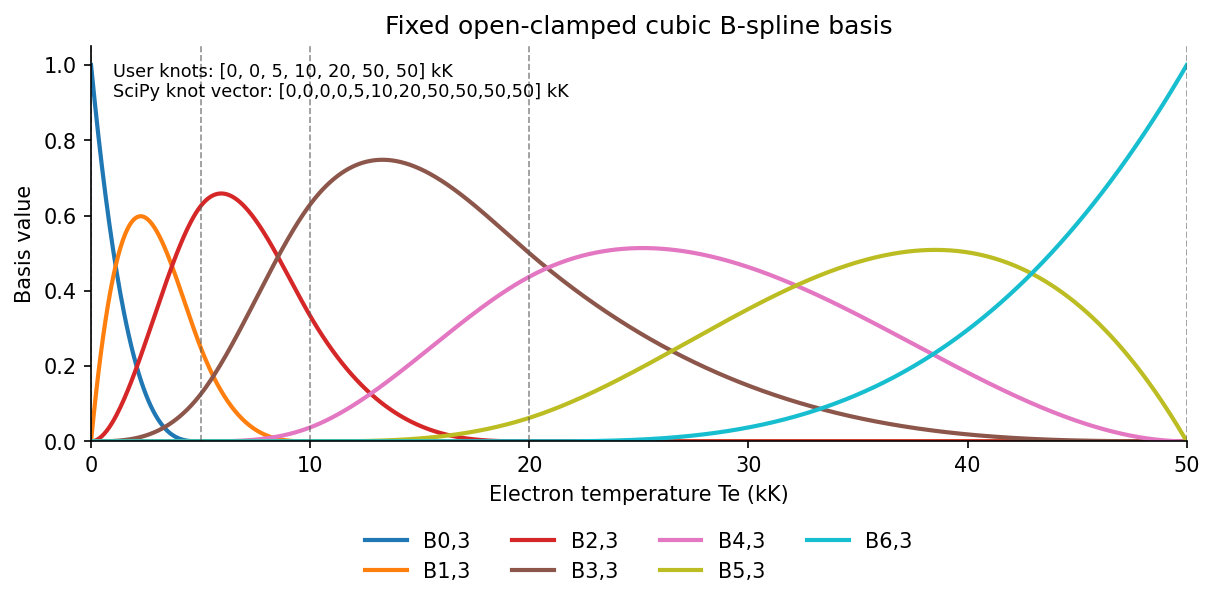
\includegraphics[width=\linewidth,height=5.05cm,keepaspectratio]{../thesis/figures/ch4/nonlinear_ttm/nonlinear_spline_basis_knots_no_greville.png}
    \end{column}
  \end{columns}
\end{frame}

\GVSetBackupSlide{D8a}
\GVSetSource{Source: thesis Ch. 4, Eqs. (4.25)--(4.27); Appendix C.}
\begin{frame}[t]{\fontsize{13}{15}\selectfont Final nonlinear 33-feature representation}
  \hypertarget{supp:sampling-feature-definitions}{}
  \vspace{-0.18cm}\hfill
  \GVBackupSectionButton{supp:sampling}{Sampling}\hspace{0.10cm}\GVBackupIndexButton
  \vspace{0.02cm}
  \begin{columns}[T,totalwidth=0.94\textwidth]
    \begin{column}{0.29\textwidth}
      \begin{beamercolorbox}[wd=\linewidth,sep=0.44em]{normal text}
        \small\textbf{\color{GVTeal}Direct scalar and geometry inputs}\par
        \vspace{0.07cm}
        \scriptsize \(F,\ k_{e0},\ C_l,\ A_e,\ B_L,\ \delta_b;\)\par
        \(L_z,\ \lambda\).
      \end{beamercolorbox}
      \vspace{0.15cm}
      \begin{beamercolorbox}[wd=\linewidth,sep=0.44em]{normal text}
        \small\textbf{\color{GVSourceBlue}Derived optical inputs}\par
        \vspace{0.07cm}\scriptsize \(\alpha_0,\ R_0\).
      \end{beamercolorbox}
    \end{column}
    \begin{column}{0.29\textwidth}
      \begin{beamercolorbox}[wd=\linewidth,sep=0.44em]{normal text}
        \small\textbf{\color{GVCapacityPurple}Nonlinear curve summaries}\par
        \vspace{0.07cm}
        \scriptsize \(C_e(300\,\mathrm K),\ G(300\,\mathrm K)\); \(\min_{\mathcal T}C_e,\max_{\mathcal T}C_e\); \(\min_{\mathcal T}G,\max_{\mathcal T}G\).\par
        \vspace{0.08cm}\tiny \(\mathcal T=\operatorname{linspace}(300,50\,000;512)\,\mathrm K\).
      \end{beamercolorbox}
    \end{column}
    \begin{column}{0.29\textwidth}
      \begin{beamercolorbox}[wd=\linewidth,sep=0.44em]{normal text}
        \small\textbf{\color{GVCapacityPurple}Log-spline coefficients}\par
        \vspace{0.07cm}
        \scriptsize \(c_0^{C_e},\ldots,c_6^{C_e}\) and \(c_0^G,\ldots,c_6^G\).\par
        \vspace{0.08cm}\tiny \(c_4^Q=c_5^Q=c_6^Q\) for the high-temperature tail.
      \end{beamercolorbox}
    \end{column}
  \end{columns}
  \vspace{0.16cm}
  \begin{beamercolorbox}[wd=0.92\textwidth,sep=0.52em]{normal text}
    \small\textbf{\color{GVCouplingOrange}Source-term-informed features}\hfill\textbf{\color{GVTitleRed}33 final regression features}\par
    \vspace{0.08cm}
    \normalsize
    \[
      \alpha_{\mathrm{eff},0}=\frac{\alpha_0}{1+\alpha_0\delta_b},\qquad
      \chi_{S,0}=\frac{\alpha_{\mathrm{eff},0}(1-R_0)}{1-\exp(-\alpha_{\mathrm{eff},0}L_z)},\qquad
      F\chi_{S,0}.
    \]
    \vspace{-0.03cm}
    \scriptsize The Lorentz--Drude descriptors \(\omega_p,(f_i,\gamma_i,\Omega_i)\), and \(z_5\) generate \(\alpha_0\) and \(R_0\), but are not retained as separate inputs in the final 33-feature model matrix.
  \end{beamercolorbox}
\end{frame}

\GVSetBackupSlide{D8b}
\GVSetSource{Public-source policy; see \texttt{docs/ASSET\_PROVENANCE.md}.}
\begin{frame}[t]{Compact selected-feature correlation diagnostic}
  \hypertarget{supp:sampling-feature-correlation}{}
  \vspace{-0.18cm}\hfill
  \GVBackupSectionButton{supp:sampling}{Sampling}\hspace{0.10cm}\GVBackupIndexButton
  \vfill
  \GVOmissionNotice{Generated correlation diagnostic omitted from public source because its input provenance is not public.}
  \vfill
\end{frame}

\GVSetBackupSlide{E0}
\GVSetSource{}
\begin{frame}[t]{E. Surrogate configurations and validation results}
  \hypertarget{supp:surrogates}{}
  \vspace{-0.20cm}\hfill\GVBackupIndexButton
  \vspace{0.08cm}
  \begin{columns}[T,totalwidth=0.94\textwidth]
    \begin{column}{0.43\textwidth}
      \small\textbf{\color{GVCapacityPurple}Model development}\par
      \vspace{0.10cm}
      \hyperlink{supp:surrogates-training-workflow}{\tikz[baseline=-0.55ex]\node[draw=GVCapacityPurple,fill=GVCanvas,rounded corners=2pt,align=left,inner xsep=5pt,inner ysep=3pt,font=\scriptsize,text width=4.65cm]{\textbf{E1} Training/model-selection workflow};}\par\vspace{0.10cm}
      \hyperlink{supp:surrogates-architectures}{\tikz[baseline=-0.55ex]\node[draw=GVCapacityPurple,fill=GVCanvas,rounded corners=2pt,align=left,inner xsep=5pt,inner ysep=3pt,font=\scriptsize,text width=4.65cm]{\textbf{E2a} Surrogate architectures};}\par\vspace{0.10cm}
      \hyperlink{supp:surrogates-linear-hpo}{\tikz[baseline=-0.55ex]\node[draw=GVCapacityPurple,fill=GVCanvas,rounded corners=2pt,align=left,inner xsep=5pt,inner ysep=3pt,font=\scriptsize,text width=4.65cm]{\textbf{E2b} Linear Optuna configurations};}\par\vspace{0.10cm}
      \hyperlink{supp:surrogates-nonlinear-configs}{\tikz[baseline=-0.55ex]\node[draw=GVCapacityPurple,fill=GVCanvas,rounded corners=2pt,align=left,inner xsep=5pt,inner ysep=3pt,font=\scriptsize,text width=4.65cm]{\textbf{E3} Nonlinear fixed configurations};}
    \end{column}
    \begin{column}{0.47\textwidth}
      \small\textbf{\color{GVCouplingOrange}Validation and threshold evidence}\par
      \vspace{0.10cm}
      \begin{columns}[T,totalwidth=\linewidth]
        \begin{column}{0.48\linewidth}
          \hyperlink{supp:surrogates-linear-metrics}{\tikz[baseline=-0.55ex]\node[draw=GVCouplingOrange,fill=GVCanvas,rounded corners=2pt,align=left,inner xsep=4pt,inner ysep=3pt,font=\scriptsize,text width=2.40cm]{\textbf{E4} Linear metrics};}\par\vspace{0.10cm}
          \hyperlink{supp:surrogates-linear-support}{\tikz[baseline=-0.55ex]\node[draw=GVCouplingOrange,fill=GVCanvas,rounded corners=2pt,align=left,inner xsep=4pt,inner ysep=3pt,font=\scriptsize,text width=2.40cm]{\textbf{E5a} Linear material support};}\par\vspace{0.10cm}
          \hyperlink{supp:surrogates-linear-threshold-intervals}{\tikz[baseline=-0.55ex]\node[draw=GVCouplingOrange,fill=GVCanvas,rounded corners=2pt,align=left,inner xsep=4pt,inner ysep=3pt,font=\scriptsize,text width=2.40cm]{\textbf{E5b} Linear threshold intervals};}
        \end{column}
        \begin{column}{0.48\linewidth}
          \hyperlink{supp:surrogates-nonlinear-material-metrics}{\tikz[baseline=-0.55ex]\node[draw=GVCouplingOrange,fill=GVCanvas,rounded corners=2pt,align=left,inner xsep=4pt,inner ysep=3pt,font=\scriptsize,text width=2.40cm]{\textbf{E6} Nonlinear availability and metrics};}\par\vspace{0.10cm}
          \hyperlink{supp:surrogates-external-comparison}{\tikz[baseline=-0.55ex]\node[draw=GVCouplingOrange,fill=GVCanvas,rounded corners=2pt,align=left,inner xsep=4pt,inner ysep=3pt,font=\scriptsize,text width=2.40cm]{\textbf{E8a} External comparison note};}\par\vspace{0.10cm}
          \hyperlink{supp:surrogates-high-grid-thresholds}{\tikz[baseline=-0.55ex]\node[draw=GVCouplingOrange,fill=GVCanvas,rounded corners=2pt,align=left,inner xsep=4pt,inner ysep=3pt,font=\scriptsize,text width=2.40cm]{\textbf{E8b} High-grid direct thresholds};}
        \end{column}
      \end{columns}
    \end{column}
  \end{columns}
\end{frame}

\GVSetBackupSlide{E1}
\GVSetSource{Source: thesis Ch. 4, Algorithm 4 and Eq. (4.10); final linear and nonlinear training records.}
\begin{frame}[t]{Training and model-selection workflow}
  \hypertarget{supp:surrogates-training-workflow}{}
  \vspace{-0.18cm}\hfill
  \GVBackupSectionButton{supp:surrogates}{Surrogates}\hspace{0.10cm}\GVBackupIndexButton
  \vspace{0.06cm}
  \begin{center}
    \begin{tikzpicture}[>=stealth,
      flowstep/.style={draw=GVTeal,fill=GVTealTint,rounded corners=2pt,align=center,font=\scriptsize,minimum height=0.63cm,minimum width=2.25cm}]
      \node[flowstep] (data) {labelled pTTM responses\\\((\boldsymbol\theta_i,T_{l,\max,i})\)};
      \node[flowstep,right=0.32cm of data] (split) {route-specific\\data split};
      \node[flowstep,right=0.32cm of split] (fit) {fit candidate\\surrogate models};
      \node[flowstep,right=0.32cm of fit] (select) {select by validation\\RMSE where available};
      \node[flowstep,right=0.32cm of select] (test) {one held-out\\test evaluation};
      \draw[->,color=GVTeal,line width=0.55pt] (data)--(split);
      \draw[->,color=GVTeal,line width=0.55pt] (split)--(fit);
      \draw[->,color=GVTeal,line width=0.55pt] (fit)--(select);
      \draw[->,color=GVTeal,line width=0.55pt] (select)--(test);
    \end{tikzpicture}
  \end{center}
  \vspace{0.16cm}
  \begin{columns}[T,totalwidth=0.94\textwidth]
    \begin{column}{0.44\textwidth}
      \begin{beamercolorbox}[wd=\linewidth,sep=0.56em]{normal text}
        \small\textbf{\color{GVCapacityPurple}Linear route}\par
        \vspace{0.08cm}\scriptsize
        \textbf{Split:} \(156{,}045\) train; \(19{,}506\) validation; \(19{,}506\) held-out test.\par
        \vspace{0.10cm}
        \textbf{Selection:} Optuna minimises validation RMSE; MLP pruning is used.\par
        \vspace{0.08cm}
        \textbf{Refit:} after selection, the chosen configuration is refit on train + validation.\par
        \vspace{0.08cm}
        \textbf{Boundary:} the held-out test set remains untouched.
      \end{beamercolorbox}
    \end{column}
    \begin{column}{0.44\textwidth}
      \begin{beamercolorbox}[wd=\linewidth,sep=0.56em]{normal text}
        \small\textbf{\color{GVCouplingOrange}Nonlinear route}\par
        \vspace{0.08cm}\scriptsize
        \textbf{Split:} \(16{,}000\) train; \(4{,}000\) held-out test; deterministic \texttt{random\_state=42}.\par
        \vspace{0.10cm}
        \textbf{Selection:} fixed bounded configurations; no full nonlinear hyperparameter optimisation.\par
        \vspace{0.10cm}
        \textbf{Boundary:} the test set remains a final evaluation partition.
      \end{beamercolorbox}
    \end{column}
  \end{columns}
\end{frame}

\GVSetBackupSlide{E2a}
\GVSetSource{Sources: Ke et al. (2017); verified project implementations; He et al. (2016).}
\begin{frame}[t]{\fontsize{13}{15}\selectfont Surrogate architectures used in the two routes}
  \hypertarget{supp:surrogates-architectures}{}
  \vspace{-0.18cm}\hfill
  \GVBackupSectionButton{supp:surrogates}{Surrogates}\hspace{0.10cm}\GVBackupIndexButton
  \vspace{0.02cm}
  \begin{columns}[T,onlytextwidth]
    \begin{column}{0.29\textwidth}
      \centering\small\textbf{\color{GVTeal}LightGBM}\par
      \vspace{0.05cm}
      \begin{tikzpicture}[>=stealth,
        n/.style={draw=GVTeal,fill=GVTealTint,rounded corners=2pt,align=center,font=\tiny,minimum width=2.42cm,inner ysep=3pt}]
        \node[n] (x) at (0,2.75) {model inputs \(\mathbf x\)};
        \node[n] (bins) at (0,2.00) {histogram bins};
        \node[n] (trees) at (0,1.25) {sequential additive\\regression trees};
        \node[n] (y) at (0,0.50) {scalar prediction\\\(\widehat T_{l,\max}\)};
        \draw[->,color=GVTeal] (x)--(bins);\draw[->,color=GVTeal] (bins)--(trees);\draw[->,color=GVTeal] (trees)--(y);
        \draw[GVSlate,line width=0.5pt] (-0.78,-0.08)--(-0.78,-0.38)--(-1.03,-0.63);\draw[GVSlate,line width=0.5pt] (-0.78,-0.38)--(-0.53,-0.63);
        \draw[GVTeal,line width=0.5pt] (0.82,-0.08)--(0.82,-0.38)--(0.57,-0.63);\draw[GVTeal,line width=0.5pt] (0.82,-0.38)--(1.07,-0.63);\draw[GVTeal,line width=0.5pt] (0.57,-0.63)--(0.45,-0.87);\draw[GVTeal,line width=0.5pt] (0.57,-0.63)--(0.69,-0.87);
        \node[font=\tiny,text=GVSlate] at (-0.78,-1.08) {depth-wise};
        \node[font=\tiny,text=GVTeal,align=center] at (0.82,-1.08) {leaf-wise\\best-first};
      \end{tikzpicture}\par
      \vspace{0.02cm}\tiny\(\widehat T_{l,\max}(\mathbf x)=f_0(\mathbf x)+\sum_m\eta h_m(\mathbf x)\).
    \end{column}
    \begin{column}{0.41\textwidth}
      \centering\small\textbf{\color{GVCapacityPurple}Linear residual MLP}\par
      \vspace{0.05cm}
      \begin{tikzpicture}[>=stealth,
        p/.style={draw=GVCapacityPurple,fill=GVCanvas,rounded corners=2pt,align=center,font=\tiny,inner xsep=4pt,inner ysep=3pt},
        b/.style={draw=GVCapacityPurple,fill=GVCanvas,rounded corners=2pt,align=center,font=\scriptsize,inner xsep=5pt,inner ysep=4pt}]
        \node[p] (scale) at (-2.00,2.55) {StandardScaler};
        \node[p] (proj) at (-0.60,2.55) {input projection\\\(10\!\to\!256\)};
        \node[p] (blocks) at (1.02,2.55) {residual block\\\(\times6\)};
        \node[p] (head) at (2.45,2.55) {scalar head};
        \draw[->,color=GVCapacityPurple] (scale)--(proj);\draw[->,color=GVCapacityPurple] (proj)--(blocks);\draw[->,color=GVCapacityPurple] (blocks)--(head);
        \node[b,minimum width=4.92cm] (res) at (0.20,1.23) {LayerNorm \(\to\) affine \(\to\) GELU \(\to\) dropout\\\(\to\) affine \(\to\) dropout};
        \draw[->,color=GVCouplingOrange,line width=0.65pt,rounded corners=3pt] (-2.35,1.23) -- (-2.35,0.46) -- (2.75,0.46) -- (2.75,1.23);
        \node[font=\tiny,text=GVCouplingOrange] at (0.20,0.24) {skip connection};
        \node[font=\scriptsize,text=GVCapacityPurple] at (0.20,-0.24) {\(z^{\ell+1}=z^\ell+g_\ell(z^\ell)\)};
      \end{tikzpicture}
    \end{column}
    \begin{column}{0.245\textwidth}
      \centering\scriptsize\textbf{\color{GVCouplingOrange}Nonlinear standard MLP}\par
      \vspace{0.05cm}
      \begin{tikzpicture}[>=stealth,
        n/.style={draw=GVCouplingOrange,fill=GVCanvas,rounded corners=2pt,align=center,font=\tiny,minimum width=2.00cm,inner ysep=3pt}]
        \node[n] (s) at (0,2.65) {StandardScaler};
        \node[n] (i) at (0,1.92) {33 inputs};
        \node[n] (h1) at (0,1.19) {hidden layer 128};
        \node[n] (h2) at (0,0.46) {hidden layer 64};
        \node[n] (o) at (0,-0.27) {scalar output \(\widehat T_{l,\max}\)};
        \draw[->,color=GVCouplingOrange] (s)--(i);\draw[->,color=GVCouplingOrange] (i)--(h1);\draw[->,color=GVCouplingOrange] (h1)--(h2);\draw[->,color=GVCouplingOrange] (h2)--(o);
      \end{tikzpicture}\par
      \vspace{0.08cm}\scriptsize\color{GVCouplingOrange}\textbf{standard MLP -- no residual connections}
    \end{column}
  \end{columns}
\end{frame}

\GVSetBackupSlide{E2b}
\GVSetSource{Source: final linear LightGBM/MLP training summaries; Optuna records.}
\begin{frame}[t]{Linear Optuna-selected model configurations}
  \hypertarget{supp:surrogates-linear-hpo}{}
  \vspace{-0.18cm}\hfill
  \GVBackupSectionButton{supp:surrogates}{Surrogates}\hspace{0.10cm}\GVBackupIndexButton
  \vspace{0.06cm}
  \begin{columns}[T,totalwidth=0.94\textwidth]
    \begin{column}{0.44\textwidth}
      \begin{beamercolorbox}[wd=\linewidth,sep=0.48em]{normal text}
        \small\textbf{\color{GVTeal}LightGBM}\hfill\scriptsize 100 trials\par
        \vspace{0.06cm}\scriptsize Selected trial 93; validation RMSE \(215.089\,\mathrm K\).\par
        \vspace{0.08cm}\scriptsize
        \begin{tabular}{@{}lr@{}}
          \texttt{num\_leaves} & 34\\
          \texttt{learning\_rate} & 0.053817\\
          \texttt{n\_estimators} & 2813\\
          \texttt{min\_child\_samples} & 54\\
          \texttt{subsample} & 0.955476\\
          \texttt{colsample\_bytree} & 0.970824\\
          \texttt{reg\_lambda} & 0.181193\\
          \texttt{reg\_alpha} & 0.0060516
        \end{tabular}
      \end{beamercolorbox}
    \end{column}
    \begin{column}{0.44\textwidth}
      \begin{beamercolorbox}[wd=\linewidth,sep=0.48em]{normal text}
        \small\textbf{\color{GVCapacityPurple}Residual MLP}\hfill\scriptsize 50 trials\par
        \vspace{0.06cm}\scriptsize 26 complete; 24 pruned.\par
        \scriptsize\textbf{Optuna trial-34 objective RMSE: \(89.5895\,\mathrm K\).}\par
        \vspace{0.08cm}\scriptsize
        \begin{tabular}{@{}lr@{}}
          \texttt{hidden\_dim} & 256\\
          \texttt{n\_layers} & 6\\
          \texttt{learning\_rate} & 0.00712289\\
          \texttt{weight\_decay} & \(8.48421\times10^{-6}\)\\
          \texttt{dropout} & 0.000299682\\
          \texttt{batch\_size} & 512
        \end{tabular}
      \end{beamercolorbox}
    \end{column}
  \end{columns}
  \vspace{0.16cm}
  \begin{beamercolorbox}[wd=0.88\textwidth,sep=0.42em]{normal text}
    \scriptsize\textbf{\color{GVCapacityPurple}Final refit best validation RMSE: \(89.6790\,\mathrm K\).}\quad Final early stopping used.
  \end{beamercolorbox}
\end{frame}

\GVSetBackupSlide{E3}
\GVSetSource{Source: Appendix C model-configuration table; final \texttt{model\_metrics\_final.csv}.}
\begin{frame}[t]{Nonlinear fixed model configurations}
  \hypertarget{supp:surrogates-nonlinear-configs}{}
  \vspace{-0.18cm}\hfill
  \GVBackupSectionButton{supp:surrogates}{Surrogates}\hspace{0.10cm}\GVBackupIndexButton
  \vspace{0.06cm}
  \begin{columns}[T,totalwidth=0.94\textwidth]
    \begin{column}{0.52\textwidth}
      \begin{beamercolorbox}[wd=\linewidth,sep=0.45em]{normal text}
        \small\textbf{\color{GVTeal}LightGBM}\par
        \vspace{0.07cm}\scriptsize
        \begin{tabular}{@{}lrlr@{}}
          \texttt{boosting\_type} & \texttt{gbdt} & \texttt{n\_estimators} & 500\\
          \texttt{learning\_rate} & 0.04 & \texttt{num\_leaves} & 63\\
          \texttt{max\_depth} & -1 & \texttt{min\_child\_samples} & 20\\
          \texttt{min\_child\_weight} & 0.001 & \texttt{min\_split\_gain} & 0.0\\
          \texttt{subsample} & 0.9 & \texttt{subsample\_freq} & 0\\
          \texttt{colsample\_bytree} & 0.9 & \texttt{reg\_alpha} & 0.001\\
          \texttt{reg\_lambda} & 0.01 & \texttt{subsample\_for\_bin} & 200000\\
          \texttt{random\_state} & 42 & \texttt{n\_jobs} & 1
        \end{tabular}
      \end{beamercolorbox}
    \end{column}
    \begin{column}{0.36\textwidth}
      \begin{beamercolorbox}[wd=\linewidth,sep=0.45em]{normal text}
        \small\textbf{\color{GVCouplingOrange}Standard MLP}\par
        \vspace{0.07cm}\scriptsize
        \begin{tabular}{@{}lr@{}}
          scaler & StandardScaler\\
          \texttt{hidden\_layer\_sizes} & [128, 64]\\
          \texttt{alpha} & 0.0001\\
          \texttt{batch\_size} & 256\\
          \texttt{early\_stopping} & true\\
          \texttt{learning\_rate\_init} & 0.001\\
          \texttt{max\_iter} & 350\\
          \texttt{random\_state} & 42
        \end{tabular}\par
        \vspace{0.11cm}\scriptsize\color{GVCouplingOrange}\textbf{No residual connections.}
      \end{beamercolorbox}
    \end{column}
  \end{columns}
  \vspace{0.16cm}
  \begin{beamercolorbox}[wd=0.91\textwidth,sep=0.44em]{normal text}
    \scriptsize\textbf{\color{GVTitleRed}The nonlinear \(20{,}000\)-sample models use fixed bounded configurations; no full nonlinear Optuna study was performed.}\par
    \vspace{0.05cm}
    \tiny Other \texttt{MLPRegressor} defaults are not restated because the authoritative final configuration record preserves only the explicit settings shown above.
  \end{beamercolorbox}
\end{frame}

\GVSetBackupSlide{E4}
\GVSetSource{Source: thesis Ch. 4, Tables 4.2--4.3; final linear metric tables.}
\begin{frame}[t]{Linear held-out and material-validation metrics}
  \hypertarget{supp:surrogates-linear-metrics}{}
  \vspace{-0.18cm}\hfill
  \GVBackupSectionButton{supp:surrogates}{Surrogates}\hspace{0.10cm}\GVBackupIndexButton
  \vspace{0.03cm}
  \begin{beamercolorbox}[wd=0.92\textwidth,sep=0.42em]{normal text}
    \small\textbf{\color{GVCapacityPurple}Held-out synthetic test set \((n=19{,}506)\)}\hfill
    \scriptsize This is distinct from material validation below.\par
    \vspace{0.07cm}\centering\scriptsize
    \begin{tabular}{@{}lrrr@{}}
      \rowcolor{GVTealTint}\textbf{Model} & \textbf{RMSE (K)} & \textbf{MAE (K)} & \textbf{\(R^2\)}\\
      LightGBM & 215.230 & 101.653 & 0.990449\\
      Residual MLP & 115.190 & 20.062 & 0.997264
    \end{tabular}
  \end{beamercolorbox}
  \vspace{0.16cm}
  \begin{beamercolorbox}[wd=0.92\textwidth,sep=0.45em]{normal text}
    \small\textbf{\color{GVCouplingOrange}Material validation: \(F\leq20{,}000\,\mathrm{J\,m^{-2}}\)}\par
    \vspace{0.07cm}\centering\scriptsize
    \begin{tabular}{@{}lrrrr@{}}
      \rowcolor{GVTealTint}\textbf{Material} & \multicolumn{2}{c}{\textbf{LightGBM}} & \multicolumn{2}{c}{\textbf{Residual MLP}}\\
      \rowcolor{GVTealTint} & RMSE (K) & \(R^2\) & RMSE (K) & \(R^2\)\\
      Ag & 88.38 & 0.889 & 21.29 & 0.994\\
      Al & 328.82 & 0.984 & 235.06 & 0.992\\
      Au & 88.80 & 0.970 & 20.83 & 0.998\\
      \rowcolor{GVRedTint}Cr & 10,190.78 & 0.549 & 13,694.16 & 0.186\\
      Cu & 180.70 & 0.973 & 13.26 & 1.000\\
      \rowcolor{GVRedTint}Ni & 8,687.34 & 0.577 & 11,614.49 & 0.243\\
      \rowcolor{GVRedTint}Ti & 13,356.51 & 0.479 & 17,503.38 & 0.106
    \end{tabular}\par
    \vspace{0.07cm}\scriptsize\color{GVSlate}Highlighted rows identify the principal linear material-transfer limitations.
  \end{beamercolorbox}
\end{frame}

\GVSetBackupSlide{E5a}
\GVSetSource{Source: thesis Ch. 4, material-feature support diagnostic.}
\begin{frame}[t]{\fontsize{13}{15}\selectfont Linear material support within the synthetic feature domain}
  \hypertarget{supp:surrogates-linear-support}{}
  \vspace{-0.18cm}\hfill
  \GVBackupSectionButton{supp:surrogates}{Surrogates}\hspace{0.10cm}\GVBackupIndexButton
  \vspace{0.04cm}
  \begin{columns}[T,totalwidth=0.95\textwidth]
    \begin{column}{0.65\textwidth}
      \centering
      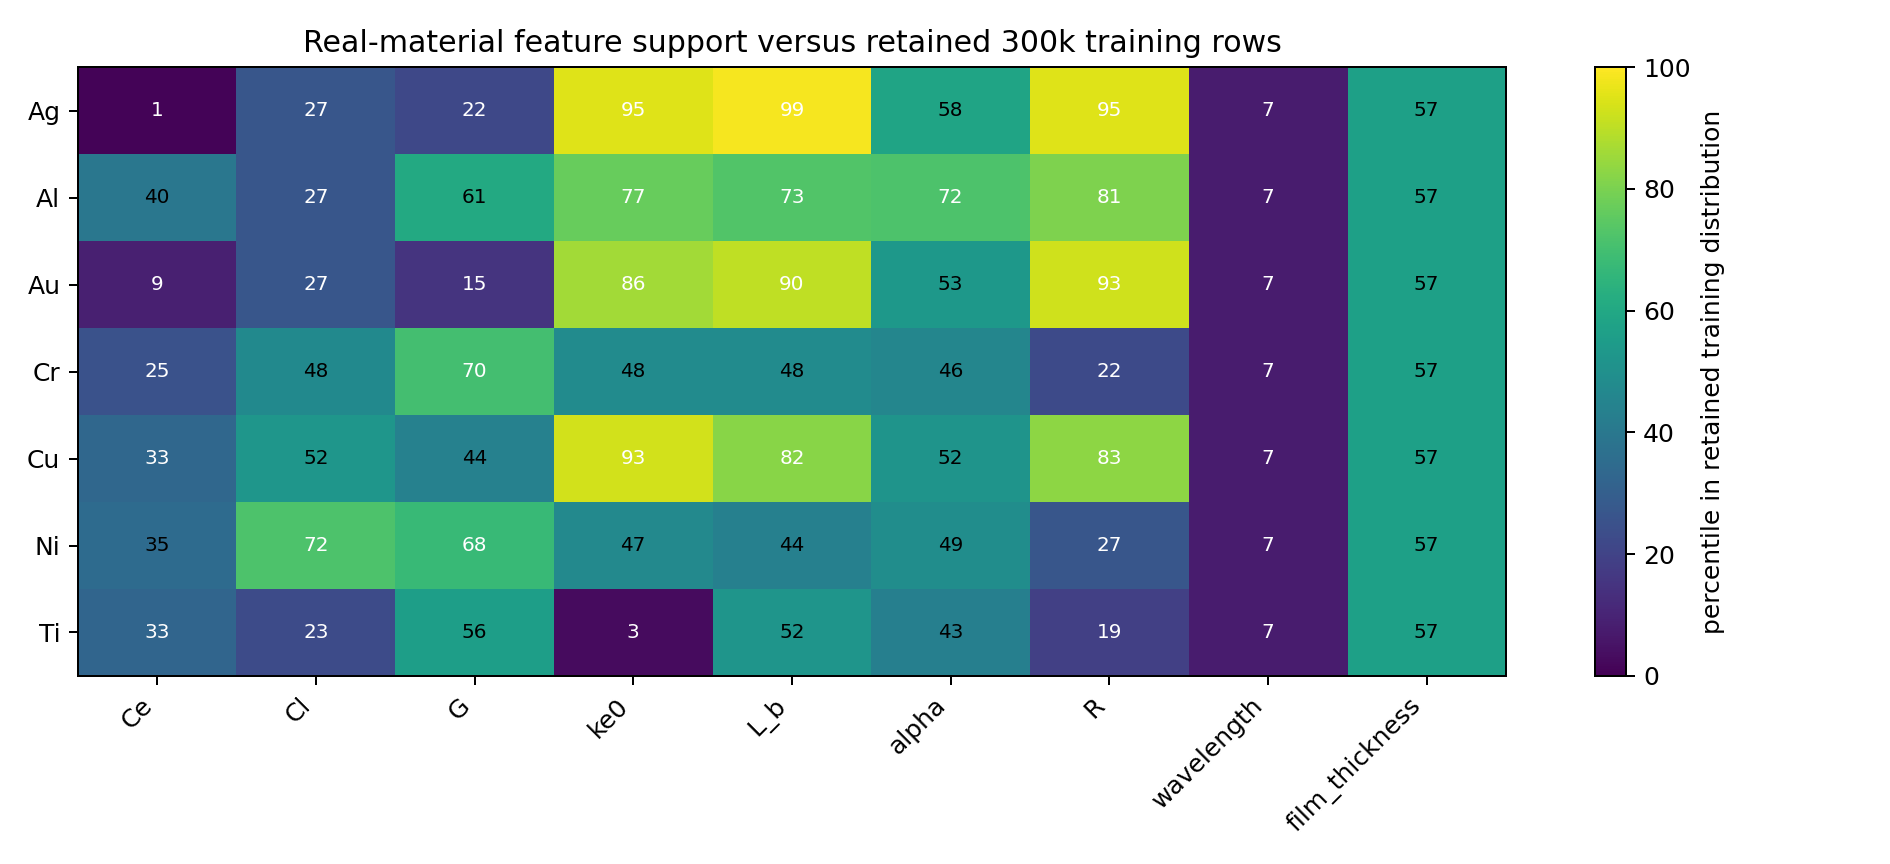
\includegraphics[width=\linewidth,height=5.45cm,keepaspectratio]{../thesis/figures/ch4/linear_ttm/material_feature_percentile_heatmap.png}
    \end{column}
    \begin{column}{0.26\textwidth}
      \begin{beamercolorbox}[wd=\linewidth,sep=0.48em]{normal text}
        \small\textbf{\color{GVTeal}Reading the diagnostic}\par
        \vspace{0.08cm}\scriptsize
        \(\bullet\) Cr, Ni, and Ti contain descriptors near or beyond the retained synthetic feature support.\par
        \vspace{0.13cm}
        \(\bullet\) Feature support is distinct from fluence support.\par
        \vspace{0.13cm}
        \(\bullet\) The map contextualises transfer errors; percentile support alone does not establish causality.
      \end{beamercolorbox}
    \end{column}
  \end{columns}
\end{frame}

\GVSetBackupSlide{E5b}
\GVSetSource{Source: thesis Ch. 4, Fig. 4.4 and Table 4.4.}
\begin{frame}[t]{\fontsize{13}{15}\selectfont Linear thresholds with residual-calibrated surrogate-error intervals}
  \hypertarget{supp:surrogates-linear-threshold-intervals}{}
  \vspace{-0.18cm}\hfill
  \GVBackupSectionButton{supp:surrogates}{Surrogates}\hspace{0.10cm}\GVBackupIndexButton
  \vspace{0.04cm}
  \begin{columns}[T,totalwidth=0.95\textwidth]
    \begin{column}{0.68\textwidth}
      \centering
      \GVOmissionNotice{External numerical comparison omitted from public source pending redistribution terms.}
    \end{column}
    \begin{column}{0.23\textwidth}
      \begin{beamercolorbox}[wd=\linewidth,sep=0.50em]{normal text}
        \small\textbf{\color{GVTitleRed}Scope of the intervals}\par
        \vspace{0.09cm}\scriptsize
        Intervals are calibrated from residuals relative to the linear numerical target.\par
        \vspace{0.14cm}
        They are not experimental uncertainty and do not quantify nonlinear model-form discrepancy.
      \end{beamercolorbox}
    \end{column}
  \end{columns}
\end{frame}

\GVSetBackupSlide{E6}
\GVSetSource{Source: Appendix C, nonlinear material-availability and material-metric tables.}
\begin{frame}[t]{Nonlinear material availability and validation metrics}
  \hypertarget{supp:surrogates-nonlinear-material-metrics}{}
  \vspace{-0.18cm}\hfill
  \GVBackupSectionButton{supp:surrogates}{Surrogates}\hspace{0.10cm}\GVBackupIndexButton
  \vspace{0.04cm}
  \begin{columns}[T,totalwidth=0.95\textwidth]
    \begin{column}{0.30\textwidth}
      \begin{beamercolorbox}[wd=\linewidth,sep=0.45em]{normal text}
        \small\textbf{\color{GVTeal}Material availability}\par
        \vspace{0.08cm}\centering\scriptsize
        \begin{tabular}{@{}lcc@{}}
          \rowcolor{GVTealTint}\textbf{Material} & \(C_e/G\) & Direct curve\\
          Ag & yes & yes\\
          Au & yes & yes\\
          Cu & yes & yes\\
          Ni & yes & yes\\
          Ti & yes & yes\\
          \rowcolor{GVRedTint}Cr & no & no\\
          \rowcolor{GVRedTint}Al & no & no
        \end{tabular}\par
        \vspace{0.10cm}\scriptsize Cr/Al are unavailable because compatible nonlinear \(C_e/G\) curves are absent from the supplied material set.
      \end{beamercolorbox}
    \end{column}
    \begin{column}{0.59\textwidth}
      \begin{beamercolorbox}[wd=\linewidth,sep=0.45em]{normal text}
        \small\textbf{\color{GVCouplingOrange}Available-material validation}\hfill\scriptsize RMSE / MAE / \(R^2\)\par
        \vspace{0.07cm}\centering\tiny
        \begin{tabular}{@{}lrrr|rrr@{}}
          \rowcolor{GVTealTint}\textbf{Material} & \multicolumn{3}{c|}{\textbf{LightGBM}} & \multicolumn{3}{c}{\textbf{Standard MLP}}\\
          \rowcolor{GVTealTint} & RMSE & MAE & \(R^2\) & RMSE & MAE & \(R^2\)\\
          Ag & 354.943 & 135.266 & 0.438 & 268.714 & 89.939 & 0.678\\
          Au & 1,693.643 & 515.535 & 0.269 & 1,765.201 & 587.993 & 0.206\\
          Cu & 769.851 & 229.272 & 0.434 & 796.774 & 288.212 & 0.394\\
          Ni & 234.346 & 109.586 & 0.986 & 217.462 & 152.604 & 0.988\\
          Ti & 169.601 & 113.626 & 0.993 & 309.705 & 166.363 & 0.976
        \end{tabular}\par
        \vspace{0.08cm}\scriptsize Direct nonlinear pTTM curves provide the material-validation reference; unavailable materials are not failed predictions.
      \end{beamercolorbox}
    \end{column}
  \end{columns}
\end{frame}

\GVSetBackupSlide{E8a}
\GVSetSource{Public-source policy; see \texttt{docs/ASSET\_PROVENANCE.md}.}
\begin{frame}[t]{External nonlinear comparison}
  \hypertarget{supp:surrogates-external-comparison}{}
  \vspace{-0.18cm}\hfill
  \GVBackupSectionButton{supp:surrogates}{Surrogates}\hspace{0.10cm}\GVBackupIndexButton
  \vfill
  \GVOmissionNotice{External PLAN-hub/RIANA numerical comparison omitted from public source pending redistribution terms.}
  \vfill
\end{frame}

\GVSetBackupSlide{E8b}
\GVSetSource{Public-source policy; see \texttt{docs/ASSET\_PROVENANCE.md}.}
\begin{frame}[t]{Two-grid sensitivity: public-source limitation}
  \hypertarget{supp:surrogates-high-grid-thresholds}{}
  \vspace{-0.18cm}\hfill
  \GVBackupSectionButton{supp:surrogates}{Surrogates}\hspace{0.10cm}\GVBackupIndexButton
  \vfill
  \GVOmissionNotice{External PLAN-hub/RIANA numerical comparison omitted from public source pending redistribution terms.}
  \vfill
\end{frame}

\end{document}
